%% Meta-Radiology submission (KeAi / Elsevier), Elsevier CAS double-column class (els-cas-templates v2.4).
%% Build from this directory:  TEXINPUTS=.:..//: BIBINPUTS=..: latexmk -pdf main.tex
\PassOptionsToPackage{table}{xcolor}
\PassOptionsToPackage{hyperfootnotes=false}{hyperref}
\documentclass[a4paper,fleqn]{cas-dc}

% Numbered references in order of appearance, cited by superscript numerals (journal style, AMA-like list).
\usepackage[numbers,super,sort&compress]{natbib}
\setcitestyle{super}

\usepackage[T1]{fontenc}
\usepackage[utf8]{inputenc}
\usepackage{microtype}
\usepackage{graphicx}
\usepackage[export]{adjustbox}
\usepackage{booktabs}
\usepackage{multirow}
\usepackage{placeins}
\usepackage{stfloats}
\usepackage{longtable}
\usepackage{enumitem}
\usepackage{amsmath}
\usepackage{xcolor}
\usepackage{url}

\graphicspath{{../}}
% One type family throughout: tables, captions and headings (sans in the stock CAS layout) use the STIX text
% face of the body, which is also the face of the figure labels (STIX / Nimbus Roman).
\renewcommand{\sfdefault}{\rmdefault}
\newcommand{\R}{\mathbb{R}}
\newcommand{\E}{\mathbb{E}}
\newcommand{\hvec}{\mathbf{h}}
\newcommand{\wvec}{\mathbf{w}}
\newcommand{\vvec}{\mathbf{v}}
\newcommand{\DeltaEff}{\Delta_{\mathrm{Eff}}}
\DeclareMathOperator*{\argmaxop}{arg\,max}
% One type size for every table. \fitwidth only ever shrinks, so a table wider than the line was
% set small and a narrow one was left at body size: across the paper the rendered table text ran from
% 7.1 pt to 10.0 pt, and the three ownership tables sat at the top of that range. At 8 pt with 3 pt
% column separation the widest table measures 453 pt against a 455 pt line, so no table is scaled at
% all and they all print at the same size. 8 pt is the largest size for which that holds.
\providecommand{\cftabsize}{\fontsize{8}{9.6}\selectfont}

% Shrink a table to the line, and to the page when it is the height that does not fit --
% table_cf_attr is 58 rows and overflowed a float page by 3.6pt once its width was fitted.
% max width/max totalheight only ever shrink, so a narrow table is left at body size.
\providecommand{\fitwidth}[1]{\adjustbox{max width=\linewidth,max totalheight=0.93\textheight}{#1}}

% terracotta = positive / high, blue = negative / low, sage = magnitude of Read and Ans; darker = larger magnitude
\definecolor{cfSage1}{HTML}{ECF3EF}
\definecolor{cfSage2}{HTML}{D5E5DB}
\definecolor{cfSage3}{HTML}{B9D4C3}
\definecolor{cfSage4}{HTML}{9EC3AC}
\definecolor{cfSlate1}{HTML}{EAF0F6}
\definecolor{cfSlate2}{HTML}{D0DDEA}
\definecolor{cfSlate3}{HTML}{B1C7DD}
\definecolor{cfSlate4}{HTML}{94B2D0}
\definecolor{cfTerra1}{HTML}{F7ECEA}
\definecolor{cfTerra2}{HTML}{EED5D1}
\definecolor{cfTerra3}{HTML}{E2B8B2}
\definecolor{cfTerra4}{HTML}{D79E95}
\definecolor{cfOat1}{HTML}{F4EFE6}
\definecolor{cfOat2}{HTML}{E8DDC8}
\definecolor{cfGrey}{HTML}{E4E1DC}

% Generated by scripts/build_numbers.py from runs/manifest.csv; do not edit.
% Rule: a block enters the write-matrix counts iff run.json completed_modules contains CORE and CALIBRATION;
% readability counts run over probe-graded cells (CALIBRATION completed). See scripts/cf_inclusion.py.
% 75 blocks, 75 included, 450 write-matrix cells, 450 probe-graded cells.
\providecommand{\cfCheckpoints}{}\renewcommand{\cfCheckpoints}{25}
\providecommand{\cfBlocks}{}\renewcommand{\cfBlocks}{75}
\providecommand{\cfWriteBlocks}{}\renewcommand{\cfWriteBlocks}{75}
\providecommand{\cfProbeBlocks}{}\renewcommand{\cfProbeBlocks}{75}
\providecommand{\cfCells}{}\renewcommand{\cfCells}{450}
\providecommand{\cfProbeCells}{}\renewcommand{\cfProbeCells}{450}
\providecommand{\cfChestBlocks}{}\renewcommand{\cfChestBlocks}{50}
\providecommand{\cfChestProbeBlocks}{}\renewcommand{\cfChestProbeBlocks}{50}
\providecommand{\cfNihBlocks}{}\renewcommand{\cfNihBlocks}{25}
\providecommand{\cfChexBlocks}{}\renewcommand{\cfChexBlocks}{25}
\providecommand{\cfCocoBlocks}{}\renewcommand{\cfCocoBlocks}{25}
\providecommand{\cfCheckpointsComplete}{}\renewcommand{\cfCheckpointsComplete}{25}
\providecommand{\cfCheckpointsCompleteWord}{}\renewcommand{\cfCheckpointsCompleteWord}{Twenty-five}
\providecommand{\cfChestReadable}{}\renewcommand{\cfChestReadable}{256}
\providecommand{\cfChestReadableN}{}\renewcommand{\cfChestReadableN}{300}
\providecommand{\cfChestReadablePct}{}\renewcommand{\cfChestReadablePct}{85}
\providecommand{\cfChestAnswerable}{}\renewcommand{\cfChestAnswerable}{257}
\providecommand{\cfChestAnswerableN}{}\renewcommand{\cfChestAnswerableN}{300}
\providecommand{\cfChestCellsN}{}\renewcommand{\cfChestCellsN}{300}
\providecommand{\cfChestAnswerablePct}{}\renewcommand{\cfChestAnswerablePct}{86}
\providecommand{\cfChestOwned}{}\renewcommand{\cfChestOwned}{44}
\providecommand{\cfChestOwnedPct}{}\renewcommand{\cfChestOwnedPct}{15}
\providecommand{\cfChestCompetitor}{}\renewcommand{\cfChestCompetitor}{219}
\providecommand{\cfChestCompetitorPct}{}\renewcommand{\cfChestCompetitorPct}{73}
\providecommand{\cfChestRefMet}{}\renewcommand{\cfChestRefMet}{56}
\providecommand{\cfChestRefBelow}{}\renewcommand{\cfChestRefBelow}{244}
\providecommand{\cfChestRefNotOwned}{}\renewcommand{\cfChestRefNotOwned}{12}
\providecommand{\cfChestRefStrong}{}\renewcommand{\cfChestRefStrong}{12}
\providecommand{\cfChestRefUnres}{}\renewcommand{\cfChestRefUnres}{0}
\providecommand{\cfChestBelowAdv}{}\renewcommand{\cfChestBelowAdv}{37}
\providecommand{\cfChestBelowStrong}{}\renewcommand{\cfChestBelowStrong}{207}
\providecommand{\cfChestBelowUnres}{}\renewcommand{\cfChestBelowUnres}{0}
\providecommand{\cfReadAnsRefMet}{}\renewcommand{\cfReadAnsRefMet}{50}
\providecommand{\cfReadAnsRefBelow}{}\renewcommand{\cfReadAnsRefBelow}{188}
\providecommand{\cfReadAnsCompetitor}{}\renewcommand{\cfReadAnsCompetitor}{170}
\providecommand{\cfReadAnsRefStrong}{}\renewcommand{\cfReadAnsRefStrong}{10}
\providecommand{\cfReadAnsRefUnres}{}\renewcommand{\cfReadAnsRefUnres}{0}
\providecommand{\cfReadAnsBelowAdv}{}\renewcommand{\cfReadAnsBelowAdv}{28}
\providecommand{\cfReadAnsBelowStrong}{}\renewcommand{\cfReadAnsBelowStrong}{160}
\providecommand{\cfReadAnsBelowUnres}{}\renewcommand{\cfReadAnsBelowUnres}{0}
\providecommand{\cfCocoRefStrong}{}\renewcommand{\cfCocoRefStrong}{0}
\providecommand{\cfCocoRefUnres}{}\renewcommand{\cfCocoRefUnres}{0}
\providecommand{\cfCocoBelowAdv}{}\renewcommand{\cfCocoBelowAdv}{12}
\providecommand{\cfCocoBelowStrong}{}\renewcommand{\cfCocoBelowStrong}{21}
\providecommand{\cfCocoBelowUnres}{}\renewcommand{\cfCocoBelowUnres}{0}
\providecommand{\cfChestBelowStrongPct}{}\renewcommand{\cfChestBelowStrongPct}{95}
\providecommand{\cfReadAns}{}\renewcommand{\cfReadAns}{238}
\providecommand{\cfReadAnsOwned}{}\renewcommand{\cfReadAnsOwned}{40}
\providecommand{\cfReadAnsOwnedPct}{}\renewcommand{\cfReadAnsOwnedPct}{17}
\providecommand{\cfRestN}{}\renewcommand{\cfRestN}{62}
\providecommand{\cfRestOwned}{}\renewcommand{\cfRestOwned}{4}
\providecommand{\cfRestOwnedPct}{}\renewcommand{\cfRestOwnedPct}{6}
\providecommand{\cfChestFloored}{}\renewcommand{\cfChestFloored}{18}
\providecommand{\cfChestFlooredPct}{}\renewcommand{\cfChestFlooredPct}{6}
\providecommand{\cfEffusionOwnedBlocks}{}\renewcommand{\cfEffusionOwnedBlocks}{8}
\providecommand{\cfEffusionOwnedSmall}{}\renewcommand{\cfEffusionOwnedSmall}{7}
\providecommand{\cfSelEffusion}{}\renewcommand{\cfSelEffusion}{0.18}
\providecommand{\cfSelCardiomegaly}{}\renewcommand{\cfSelCardiomegaly}{0.19}
\providecommand{\cfSelChestMed}{}\renewcommand{\cfSelChestMed}{0.14}
\providecommand{\cfSelChestQOne}{}\renewcommand{\cfSelChestQOne}{0.08}
\providecommand{\cfSelChestQThree}{}\renewcommand{\cfSelChestQThree}{0.22}
\providecommand{\cfSelChestN}{}\renewcommand{\cfSelChestN}{300}
\providecommand{\cfNihReadable}{}\renewcommand{\cfNihReadable}{135}
\providecommand{\cfNihReadableN}{}\renewcommand{\cfNihReadableN}{150}
\providecommand{\cfNihCells}{}\renewcommand{\cfNihCells}{150}
\providecommand{\cfNihAnswerable}{}\renewcommand{\cfNihAnswerable}{143}
\providecommand{\cfNihOwned}{}\renewcommand{\cfNihOwned}{16}
\providecommand{\cfNihCompetitor}{}\renewcommand{\cfNihCompetitor}{112}
\providecommand{\cfNihRefMet}{}\renewcommand{\cfNihRefMet}{20}
\providecommand{\cfMedianWqqNih}{}\renewcommand{\cfMedianWqqNih}{0.010}
\providecommand{\cfOwnShareNih}{}\renewcommand{\cfOwnShareNih}{24}
\providecommand{\cfChexReadable}{}\renewcommand{\cfChexReadable}{121}
\providecommand{\cfChexReadableN}{}\renewcommand{\cfChexReadableN}{150}
\providecommand{\cfChexCells}{}\renewcommand{\cfChexCells}{150}
\providecommand{\cfChexAnswerable}{}\renewcommand{\cfChexAnswerable}{114}
\providecommand{\cfChexOwned}{}\renewcommand{\cfChexOwned}{28}
\providecommand{\cfChexCompetitor}{}\renewcommand{\cfChexCompetitor}{107}
\providecommand{\cfChexRefMet}{}\renewcommand{\cfChexRefMet}{36}
\providecommand{\cfMedianWqqChex}{}\renewcommand{\cfMedianWqqChex}{0.020}
\providecommand{\cfOwnShareChex}{}\renewcommand{\cfOwnShareChex}{22}
\providecommand{\cfCocoReadable}{}\renewcommand{\cfCocoReadable}{118}
\providecommand{\cfCocoReadableN}{}\renewcommand{\cfCocoReadableN}{150}
\providecommand{\cfCocoCells}{}\renewcommand{\cfCocoCells}{150}
\providecommand{\cfCocoAnswerable}{}\renewcommand{\cfCocoAnswerable}{121}
\providecommand{\cfCocoOwned}{}\renewcommand{\cfCocoOwned}{117}
\providecommand{\cfCocoCompetitor}{}\renewcommand{\cfCocoCompetitor}{21}
\providecommand{\cfCocoRefMet}{}\renewcommand{\cfCocoRefMet}{117}
\providecommand{\cfMedianWqqCoco}{}\renewcommand{\cfMedianWqqCoco}{0.127}
\providecommand{\cfOwnShareCoco}{}\renewcommand{\cfOwnShareCoco}{79}
\providecommand{\cfCocoOwnedN}{}\renewcommand{\cfCocoOwnedN}{150}
\providecommand{\cfCocoOwnedPct}{}\renewcommand{\cfCocoOwnedPct}{78}
\providecommand{\cfCocoAnswerablePct}{}\renewcommand{\cfCocoAnswerablePct}{81}
\providecommand{\cfCocoFloored}{}\renewcommand{\cfCocoFloored}{86}
\providecommand{\cfCocoFlooredPct}{}\renewcommand{\cfCocoFlooredPct}{57}
\providecommand{\cfCocoBlocksFourPlus}{}\renewcommand{\cfCocoBlocksFourPlus}{19}
\providecommand{\cfAltdirBlocks}{}\renewcommand{\cfAltdirBlocks}{60}
\providecommand{\cfAltdirBlocksPerDs}{}\renewcommand{\cfAltdirBlocksPerDs}{20}
\providecommand{\cfAltdirBlocksNih}{}\renewcommand{\cfAltdirBlocksNih}{20}
\providecommand{\cfAltdirNihN}{}\renewcommand{\cfAltdirNihN}{120}
\providecommand{\cfAltdirNihLogistic}{}\renewcommand{\cfAltdirNihLogistic}{10}
\providecommand{\cfAltdirNihDom}{}\renewcommand{\cfAltdirNihDom}{22}
\providecommand{\cfAltdirNihPattern}{}\renewcommand{\cfAltdirNihPattern}{19}
\providecommand{\cfAltdirNihOrth}{}\renewcommand{\cfAltdirNihOrth}{11}
\providecommand{\cfAltdirNihResid}{}\renewcommand{\cfAltdirNihResid}{12}
\providecommand{\cfAltdirNihAny}{}\renewcommand{\cfAltdirNihAny}{33}
\providecommand{\cfAltdirBlocksChex}{}\renewcommand{\cfAltdirBlocksChex}{20}
\providecommand{\cfAltdirChexN}{}\renewcommand{\cfAltdirChexN}{120}
\providecommand{\cfAltdirChexLogistic}{}\renewcommand{\cfAltdirChexLogistic}{22}
\providecommand{\cfAltdirChexDom}{}\renewcommand{\cfAltdirChexDom}{23}
\providecommand{\cfAltdirChexPattern}{}\renewcommand{\cfAltdirChexPattern}{20}
\providecommand{\cfAltdirChexOrth}{}\renewcommand{\cfAltdirChexOrth}{16}
\providecommand{\cfAltdirChexResid}{}\renewcommand{\cfAltdirChexResid}{16}
\providecommand{\cfAltdirChexAny}{}\renewcommand{\cfAltdirChexAny}{48}
\providecommand{\cfAltdirBlocksCoco}{}\renewcommand{\cfAltdirBlocksCoco}{20}
\providecommand{\cfAltdirCocoN}{}\renewcommand{\cfAltdirCocoN}{120}
\providecommand{\cfAltdirCocoLogistic}{}\renewcommand{\cfAltdirCocoLogistic}{103}
\providecommand{\cfAltdirCocoDom}{}\renewcommand{\cfAltdirCocoDom}{69}
\providecommand{\cfAltdirCocoPattern}{}\renewcommand{\cfAltdirCocoPattern}{58}
\providecommand{\cfAltdirCocoOrth}{}\renewcommand{\cfAltdirCocoOrth}{99}
\providecommand{\cfAltdirCocoResid}{}\renewcommand{\cfAltdirCocoResid}{102}
\providecommand{\cfAltdirCocoAny}{}\renewcommand{\cfAltdirCocoAny}{110}
\providecommand{\cfAltdirChestPctMin}{}\renewcommand{\cfAltdirChestPctMin}{9}
\providecommand{\cfAltdirChestPctMax}{}\renewcommand{\cfAltdirChestPctMax}{19}
\providecommand{\cfAltdirCocoPctMin}{}\renewcommand{\cfAltdirCocoPctMin}{48}
\providecommand{\cfAltdirCocoPctMax}{}\renewcommand{\cfAltdirCocoPctMax}{85}
\providecommand{\cfFamilies}{}\renewcommand{\cfFamilies}{12}
\providecommand{\cfFamiliesWord}{}\renewcommand{\cfFamiliesWord}{twelve}
\providecommand{\cfMedicalFamilies}{}\renewcommand{\cfMedicalFamilies}{6}
\providecommand{\cfMedicalFamiliesWord}{}\renewcommand{\cfMedicalFamiliesWord}{six}
\providecommand{\cfTowerDesigns}{}\renewcommand{\cfTowerDesigns}{6}
\providecommand{\cfTowerDesignsWord}{}\renewcommand{\cfTowerDesignsWord}{six}
\providecommand{\cfTokensMin}{}\renewcommand{\cfTokensMin}{128}
\providecommand{\cfTokensMax}{}\renewcommand{\cfTokensMax}{4{,}096}
\providecommand{\cfSpecTowerN}{}\renewcommand{\cfSpecTowerN}{36}
\providecommand{\cfSpecTowerOwned}{}\renewcommand{\cfSpecTowerOwned}{7}
\providecommand{\cfSpecTowerAnswerable}{}\renewcommand{\cfSpecTowerAnswerable}{33}
\providecommand{\cfSpecTowerReadableN}{}\renewcommand{\cfSpecTowerReadableN}{36}
\providecommand{\cfSpecTowerReadable}{}\renewcommand{\cfSpecTowerReadable}{32}
\providecommand{\cfSpecTowerBlocks}{}\renewcommand{\cfSpecTowerBlocks}{6}
\providecommand{\cfSpecTowerAnsAuroc}{}\renewcommand{\cfSpecTowerAnsAuroc}{0.837}
\providecommand{\cfSpecNihTowerN}{}\renewcommand{\cfSpecNihTowerN}{18}
\providecommand{\cfSpecNihTowerOwned}{}\renewcommand{\cfSpecNihTowerOwned}{2}
\providecommand{\cfSpecMedN}{}\renewcommand{\cfSpecMedN}{72}
\providecommand{\cfSpecMedOwned}{}\renewcommand{\cfSpecMedOwned}{16}
\providecommand{\cfSpecMedAnswerable}{}\renewcommand{\cfSpecMedAnswerable}{65}
\providecommand{\cfSpecMedReadableN}{}\renewcommand{\cfSpecMedReadableN}{72}
\providecommand{\cfSpecMedReadable}{}\renewcommand{\cfSpecMedReadable}{63}
\providecommand{\cfSpecMedBlocks}{}\renewcommand{\cfSpecMedBlocks}{12}
\providecommand{\cfSpecMedAnsAuroc}{}\renewcommand{\cfSpecMedAnsAuroc}{0.797}
\providecommand{\cfSpecNihMedN}{}\renewcommand{\cfSpecNihMedN}{36}
\providecommand{\cfSpecNihMedOwned}{}\renewcommand{\cfSpecNihMedOwned}{4}
\providecommand{\cfSpecGenN}{}\renewcommand{\cfSpecGenN}{192}
\providecommand{\cfSpecGenOwned}{}\renewcommand{\cfSpecGenOwned}{21}
\providecommand{\cfSpecGenAnswerable}{}\renewcommand{\cfSpecGenAnswerable}{159}
\providecommand{\cfSpecGenReadableN}{}\renewcommand{\cfSpecGenReadableN}{192}
\providecommand{\cfSpecGenReadable}{}\renewcommand{\cfSpecGenReadable}{161}
\providecommand{\cfSpecGenBlocks}{}\renewcommand{\cfSpecGenBlocks}{32}
\providecommand{\cfSpecGenAnsAuroc}{}\renewcommand{\cfSpecGenAnsAuroc}{0.652}
\providecommand{\cfSpecNihGenN}{}\renewcommand{\cfSpecNihGenN}{96}
\providecommand{\cfSpecNihGenOwned}{}\renewcommand{\cfSpecNihGenOwned}{10}
\providecommand{\cfSpecTowerCocoN}{}\renewcommand{\cfSpecTowerCocoN}{18}
\providecommand{\cfSpecTowerCocoOwned}{}\renewcommand{\cfSpecTowerCocoOwned}{2}
\providecommand{\cfSpecTowerCocoAnswerable}{}\renewcommand{\cfSpecTowerCocoAnswerable}{11}
\providecommand{\cfSpecTowerCocoAnsAuroc}{}\renewcommand{\cfSpecTowerCocoAnsAuroc}{0.538}
\providecommand{\cfSpecMedCocoN}{}\renewcommand{\cfSpecMedCocoN}{36}
\providecommand{\cfSpecMedCocoOwned}{}\renewcommand{\cfSpecMedCocoOwned}{29}
\providecommand{\cfSpecMedCocoAnswerable}{}\renewcommand{\cfSpecMedCocoAnswerable}{30}
\providecommand{\cfSpecMedCocoAnsAuroc}{}\renewcommand{\cfSpecMedCocoAnsAuroc}{0.962}
\providecommand{\cfSpecGenCocoN}{}\renewcommand{\cfSpecGenCocoN}{96}
\providecommand{\cfSpecGenCocoOwned}{}\renewcommand{\cfSpecGenCocoOwned}{86}
\providecommand{\cfSpecGenCocoAnswerable}{}\renewcommand{\cfSpecGenCocoAnswerable}{80}
\providecommand{\cfSpecGenCocoAnsAuroc}{}\renewcommand{\cfSpecGenCocoAnsAuroc}{0.987}
\providecommand{\cfSpecTowerProbeAuroc}{}\renewcommand{\cfSpecTowerProbeAuroc}{0.855}
\providecommand{\cfSpecTowerProbeN}{}\renewcommand{\cfSpecTowerProbeN}{18}
\providecommand{\cfSpecStockProbeAuroc}{}\renewcommand{\cfSpecStockProbeAuroc}{0.773}
\providecommand{\cfSpecStockProbeN}{}\renewcommand{\cfSpecStockProbeN}{6}
\providecommand{\cfSpecRestProbeAuroc}{}\renewcommand{\cfSpecRestProbeAuroc}{0.774}
\providecommand{\cfSpecRestProbeN}{}\renewcommand{\cfSpecRestProbeN}{132}
\providecommand{\cfSpecUngradedTemplates}{}\renewcommand{\cfSpecUngradedTemplates}{6}
\providecommand{\cfSpecUngradedTemplatesWord}{}\renewcommand{\cfSpecUngradedTemplatesWord}{six}
\providecommand{\cfSpecUngradedRows}{}\renewcommand{\cfSpecUngradedRows}{16}
\providecommand{\cfGeoCosNih}{}\renewcommand{\cfGeoCosNih}{0.019}
\providecommand{\cfGeoCosRandom}{}\renewcommand{\cfGeoCosRandom}{0.024}
\providecommand{\cfGeoCosChex}{}\renewcommand{\cfGeoCosChex}{0.21}
\providecommand{\cfGeoAbsCosNih}{}\renewcommand{\cfGeoAbsCosNih}{0.093}
\providecommand{\cfGeoAbsCosChex}{}\renewcommand{\cfGeoAbsCosChex}{0.22}
\providecommand{\cfGeoAbsCosCoco}{}\renewcommand{\cfGeoAbsCosCoco}{0.058}
\providecommand{\cfGeoCosEffCons}{}\renewcommand{\cfGeoCosEffCons}{0.46}
\providecommand{\cfGeoPhiEffCons}{}\renewcommand{\cfGeoPhiEffCons}{0.74}
\providecommand{\cfGeoPhiNih}{}\renewcommand{\cfGeoPhiNih}{0.026}
\providecommand{\cfGeoOwnWinsNihPct}{}\renewcommand{\cfGeoOwnWinsNihPct}{25}
\providecommand{\cfGeoOwnWinsChexPct}{}\renewcommand{\cfGeoOwnWinsChexPct}{29}
\providecommand{\cfGeoChanceCosMin}{}\renewcommand{\cfGeoChanceCosMin}{21}
\providecommand{\cfGeoChanceCosMax}{}\renewcommand{\cfGeoChanceCosMax}{22}
\providecommand{\cfGeoChanceLabelMin}{}\renewcommand{\cfGeoChanceLabelMin}{16}
\providecommand{\cfGeoChanceLabelMax}{}\renewcommand{\cfGeoChanceLabelMax}{24}
\providecommand{\cfGeoOffdiagCells}{}\renewcommand{\cfGeoOffdiagCells}{1{,}500}
\providecommand{\cfGeoRhoAdvCos}{}\renewcommand{\cfGeoRhoAdvCos}{0.037}
\providecommand{\cfGeoRhoAdvCosP}{}\renewcommand{\cfGeoRhoAdvCosP}{0.15}
\providecommand{\cfGeoRhoAdvPhi}{}\renewcommand{\cfGeoRhoAdvPhi}{-0.001}
\providecommand{\cfGeoTwoAbove}{}\renewcommand{\cfGeoTwoAbove}{163}
\providecommand{\cfGeoTwoAboveN}{}\renewcommand{\cfGeoTwoAboveN}{300}
\providecommand{\cfGeoTwoAbovePct}{}\renewcommand{\cfGeoTwoAbovePct}{54}
\providecommand{\cfGeoCocoFamMinPct}{}\renewcommand{\cfGeoCocoFamMinPct}{91}
\providecommand{\cfGeoCocoFamMaxPct}{}\renewcommand{\cfGeoCocoFamMaxPct}{96}
\providecommand{\cfGeoCocoFamFullMinPct}{}\renewcommand{\cfGeoCocoFamFullMinPct}{82}
\providecommand{\cfGeoCocoFamFullMaxPct}{}\renewcommand{\cfGeoCocoFamFullMaxPct}{90}
\providecommand{\cfGeoFamPhiPersonBicycle}{}\renewcommand{\cfGeoFamPhiPersonBicycle}{0.14}
\providecommand{\cfGeoFamPhiPersonDog}{}\renewcommand{\cfGeoFamPhiPersonDog}{-0.06}
\providecommand{\cfGeoFamPhiChairBottle}{}\renewcommand{\cfGeoFamPhiChairBottle}{0.12}
\providecommand{\cfGeoFamPhiCarBicycle}{}\renewcommand{\cfGeoFamPhiCarBicycle}{0.13}
\providecommand{\cfGeoFamPhiPersonChairBottle}{}\renewcommand{\cfGeoFamPhiPersonChairBottle}{0.08}
\providecommand{\cfSeedCosNodule}{}\renewcommand{\cfSeedCosNodule}{-0.06}
\providecommand{\cfSeedWNodule}{}\renewcommand{\cfSeedWNodule}{0.262}
\providecommand{\cfSeedWEff}{}\renewcommand{\cfSeedWEff}{0.190}
\providecommand{\cfSeedCosAtel}{}\renewcommand{\cfSeedCosAtel}{0.49}
\providecommand{\cfSeedWAtel}{}\renewcommand{\cfSeedWAtel}{0.083}
\providecommand{\cfScaleAgree}{}\renewcommand{\cfScaleAgree}{440}
\providecommand{\cfScaleAgreeN}{}\renewcommand{\cfScaleAgreeN}{450}
\providecommand{\cfScaleOwned}{}\renewcommand{\cfScaleOwned}{161}
\providecommand{\cfScaleOwnedKeepFull}{}\renewcommand{\cfScaleOwnedKeepFull}{153}
\providecommand{\cfScaleOwnedMpos}{}\renewcommand{\cfScaleOwnedMpos}{157}
\providecommand{\cfScaleSatNih}{}\renewcommand{\cfScaleSatNih}{0.16}
\providecommand{\cfScaleSatChex}{}\renewcommand{\cfScaleSatChex}{0.10}
\providecommand{\cfScaleSatCoco}{}\renewcommand{\cfScaleSatCoco}{0.71}
\providecommand{\cfScaleUnsatGradeN}{}\renewcommand{\cfScaleUnsatGradeN}{43}
\providecommand{\cfScaleUnsatGradeKept}{}\renewcommand{\cfScaleUnsatGradeKept}{42}
\providecommand{\cfScaleUnsatGradeRef}{}\renewcommand{\cfScaleUnsatGradeRef}{42}
\providecommand{\cfScaleUnsatGradeAdv}{}\renewcommand{\cfScaleUnsatGradeAdv}{43}
\providecommand{\cfScaleUnsatGradeGained}{}\renewcommand{\cfScaleUnsatGradeGained}{1}
\providecommand{\cfScaleUnsatGradeOtherN}{}\renewcommand{\cfScaleUnsatGradeOtherN}{247}
\providecommand{\cfScaleUnsatOwned}{}\renewcommand{\cfScaleUnsatOwned}{43}
\providecommand{\cfScaleUnsatOwnedKept}{}\renewcommand{\cfScaleUnsatOwnedKept}{43}
\providecommand{\cfScaleUnsatOtherPos}{}\renewcommand{\cfScaleUnsatOtherPos}{36}
\providecommand{\cfScaleUnsatOther}{}\renewcommand{\cfScaleUnsatOther}{247}
\providecommand{\cfScaleRefitMedian}{}\renewcommand{\cfScaleRefitMedian}{0.02}
\providecommand{\cfRefitStableNih}{}\renewcommand{\cfRefitStableNih}{10}
\providecommand{\cfRefitOwnedNih}{}\renewcommand{\cfRefitOwnedNih}{16}
\providecommand{\cfRefitStableCoco}{}\renewcommand{\cfRefitStableCoco}{109}
\providecommand{\cfRefitOwnedCoco}{}\renewcommand{\cfRefitOwnedCoco}{117}
\providecommand{\cfScaleBatchMin}{}\renewcommand{\cfScaleBatchMin}{0.00}
\providecommand{\cfScaleBatchMax}{}\renewcommand{\cfScaleBatchMax}{1.84}
\providecommand{\cfScaleBatchAgree}{}\renewcommand{\cfScaleBatchAgree}{71}
\providecommand{\cfScaleBatchN}{}\renewcommand{\cfScaleBatchN}{77}
\providecommand{\cfScaleBatchDisagree}{}\renewcommand{\cfScaleBatchDisagree}{6}
\providecommand{\cfScaleBatchDisagreeOwned}{}\renewcommand{\cfScaleBatchDisagreeOwned}{1}
\providecommand{\cfScaleBaselineN}{}\renewcommand{\cfScaleBaselineN}{74}
\providecommand{\cfScaleBaselineIdentical}{}\renewcommand{\cfScaleBaselineIdentical}{44}
\providecommand{\cfScaleBaselineRestPct}{}\renewcommand{\cfScaleBaselineRestPct}{0}
\providecommand{\cfScaleBaselineDpPct}{}\renewcommand{\cfScaleBaselineDpPct}{7.7}
\providecommand{\cfConnWqqNih}{}\renewcommand{\cfConnWqqNih}{0.008}
\providecommand{\cfPrimWqqNih}{}\renewcommand{\cfPrimWqqNih}{0.032}
\providecommand{\cfConnWqqCoco}{}\renewcommand{\cfConnWqqCoco}{0.008}
\providecommand{\cfPrimWqqCoco}{}\renewcommand{\cfPrimWqqCoco}{0.127}
\providecommand{\cfPairDeltaEffFourTwelve}{}\renewcommand{\cfPairDeltaEffFourTwelve}{-0.83}
\providecommand{\cfPairDeltaEffFourTwelveLo}{}\renewcommand{\cfPairDeltaEffFourTwelveLo}{-0.85}
\providecommand{\cfPairDeltaEffFourTwelveHi}{}\renewcommand{\cfPairDeltaEffFourTwelveHi}{-0.81}
\providecommand{\cfPairDeltaEffTwelveTwentySeven}{}\renewcommand{\cfPairDeltaEffTwelveTwentySeven}{+0.79}
\providecommand{\cfPairDeltaEffTwelveTwentySevenLo}{}\renewcommand{\cfPairDeltaEffTwelveTwentySevenLo}{+0.76}
\providecommand{\cfPairDeltaEffTwelveTwentySevenHi}{}\renewcommand{\cfPairDeltaEffTwelveTwentySevenHi}{+0.82}
\providecommand{\cfPairsFiveOrSix}{}\renewcommand{\cfPairsFiveOrSix}{11}
\providecommand{\cfPairsN}{}\renewcommand{\cfPairsN}{12}
\providecommand{\cfPairsRatioMin}{}\renewcommand{\cfPairsRatioMin}{0.6}
\providecommand{\cfPairsRatioMax}{}\renewcommand{\cfPairsRatioMax}{4.6}
\providecommand{\cfPairsRatioN}{}\renewcommand{\cfPairsRatioN}{12}
\providecommand{\cfPairsRatioAboveOne}{}\renewcommand{\cfPairsRatioAboveOne}{11}
\providecommand{\cfPairsRatioSingleMax}{}\renewcommand{\cfPairsRatioSingleMax}{17.3}
\providecommand{\cfOGemmaTwelveEff}{}\renewcommand{\cfOGemmaTwelveEff}{-0.83}
\providecommand{\cfOGemmaTwelveMass}{}\renewcommand{\cfOGemmaTwelveMass}{-0.65}
\providecommand{\cfOGemmaTwelvePneu}{}\renewcommand{\cfOGemmaTwelvePneu}{-0.71}
\providecommand{\cfOGemmaTwentySevenEff}{}\renewcommand{\cfOGemmaTwentySevenEff}{-0.04}
\providecommand{\cfOGemmaTwentySevenMass}{}\renewcommand{\cfOGemmaTwentySevenMass}{-0.08}
\providecommand{\cfOGemmaTwentySevenPneu}{}\renewcommand{\cfOGemmaTwentySevenPneu}{-0.01}
\providecommand{\cfOMedFourPneu}{}\renewcommand{\cfOMedFourPneu}{-0.60}
\providecommand{\cfOMedTwentySevenPneu}{}\renewcommand{\cfOMedTwentySevenPneu}{-0.06}
\providecommand{\cfOMedFourEdema}{}\renewcommand{\cfOMedFourEdema}{+0.10}
\providecommand{\cfOMedTwentySevenEdema}{}\renewcommand{\cfOMedTwentySevenEdema}{-0.28}
\providecommand{\cfPairsGemmaFourOmNear}{}\renewcommand{\cfPairsGemmaFourOmNear}{-1.1}
\providecommand{\cfPairsGemmaFourOmFar}{}\renewcommand{\cfPairsGemmaFourOmFar}{-19.8}
\providecommand{\cfLlavaSevenCoco}{}\renewcommand{\cfLlavaSevenCoco}{5}
\providecommand{\cfLlavaThirteenCoco}{}\renewcommand{\cfLlavaThirteenCoco}{3}
\providecommand{\cfValAurocAnsNih}{}\renewcommand{\cfValAurocAnsNih}{0.64}
\providecommand{\cfValAurocProbeNih}{}\renewcommand{\cfValAurocProbeNih}{0.73}
\providecommand{\cfValAurocAnsChex}{}\renewcommand{\cfValAurocAnsChex}{0.67}
\providecommand{\cfValAurocProbeChex}{}\renewcommand{\cfValAurocProbeChex}{0.85}
\providecommand{\cfValAurocAnsClean}{}\renewcommand{\cfValAurocAnsClean}{0.89}
\providecommand{\cfValAurocProbeClean}{}\renewcommand{\cfValAurocProbeClean}{0.75}
\providecommand{\cfValCosSigmaChestMin}{}\renewcommand{\cfValCosSigmaChestMin}{0.36}
\providecommand{\cfValCosSigmaChestMax}{}\renewcommand{\cfValCosSigmaChestMax}{0.43}
\providecommand{\cfValCosSigmaCoco}{}\renewcommand{\cfValCosSigmaCoco}{0.81}
\providecommand{\cfValColSelNih}{}\renewcommand{\cfValColSelNih}{0.12}
\providecommand{\cfValColSelGeHalfNih}{}\renewcommand{\cfValColSelGeHalfNih}{2}
\providecommand{\cfValColSelNNih}{}\renewcommand{\cfValColSelNNih}{150}
\providecommand{\cfValColSelChex}{}\renewcommand{\cfValColSelChex}{0.12}
\providecommand{\cfValColSelGeHalfChex}{}\renewcommand{\cfValColSelGeHalfChex}{2}
\providecommand{\cfValColSelNChex}{}\renewcommand{\cfValColSelNChex}{150}
\providecommand{\cfValColSelCoco}{}\renewcommand{\cfValColSelCoco}{0.57}
\providecommand{\cfValColSelGeHalfCoco}{}\renewcommand{\cfValColSelGeHalfCoco}{92}
\providecommand{\cfValColSelNCoco}{}\renewcommand{\cfValColSelNCoco}{150}
\providecommand{\cfValColSelGeHalfChest}{}\renewcommand{\cfValColSelGeHalfChest}{4}
\providecommand{\cfValColSelNChest}{}\renewcommand{\cfValColSelNChest}{300}
\providecommand{\cfValKnownSignAgree}{}\renewcommand{\cfValKnownSignAgree}{143}
\providecommand{\cfValKnownN}{}\renewcommand{\cfValKnownN}{150}
\providecommand{\cfValKnownOwnedSummary}{}\renewcommand{\cfValKnownOwnedSummary}{25}
\providecommand{\cfValKnownOwnedKnown}{}\renewcommand{\cfValKnownOwnedKnown}{24}
\providecommand{\cfValKnownOwnedFull}{}\renewcommand{\cfValKnownOwnedFull}{25}
\providecommand{\cfValKnownOwnedFullAll}{}\renewcommand{\cfValKnownOwnedFullAll}{29}
\providecommand{\cfColSelNih}{}\renewcommand{\cfColSelNih}{0.12}
\providecommand{\cfColSelChex}{}\renewcommand{\cfColSelChex}{0.12}
\providecommand{\cfColSelCoco}{}\renewcommand{\cfColSelCoco}{0.57}
\providecommand{\cfColSelChestGe}{}\renewcommand{\cfColSelChestGe}{4}
\providecommand{\cfColSelChestN}{}\renewcommand{\cfColSelChestN}{300}
\providecommand{\cfColSelCocoGe}{}\renewcommand{\cfColSelCocoGe}{92}
\providecommand{\cfColSelCocoN}{}\renewcommand{\cfColSelCocoN}{150}
\providecommand{\cfKnownSignAgree}{}\renewcommand{\cfKnownSignAgree}{143}
\providecommand{\cfKnownN}{}\renewcommand{\cfKnownN}{150}
\providecommand{\cfKnownOwned}{}\renewcommand{\cfKnownOwned}{25}
\providecommand{\cfKnownOwnedKept}{}\renewcommand{\cfKnownOwnedKept}{24}
\providecommand{\cfPrecisionBlocks}{}\renewcommand{\cfPrecisionBlocks}{9}
\providecommand{\cfPrecisionPointMaxDW}{}\renewcommand{\cfPrecisionPointMaxDW}{0.044}
\providecommand{\cfPrecisionPointVerdictChanges}{}\renewcommand{\cfPrecisionPointVerdictChanges}{0}
\providecommand{\cfLabelGapCocoBlocks}{}\renewcommand{\cfLabelGapCocoBlocks}{13}
\providecommand{\cfLabelGapCocoHi}{}\renewcommand{\cfLabelGapCocoHi}{-3}
\providecommand{\cfLabelGapCocoLo}{}\renewcommand{\cfLabelGapCocoLo}{-23}
\providecommand{\cfLabelGapNihBlocks}{}\renewcommand{\cfLabelGapNihBlocks}{16}
\providecommand{\cfCoverageBlocksAllSeven}{}\renewcommand{\cfCoverageBlocksAllSeven}{74}
\providecommand{\cfCoverageChexFull}{}\renewcommand{\cfCoverageChexFull}{24}
\providecommand{\cfRefitBlocksNih}{}\renewcommand{\cfRefitBlocksNih}{25}
\providecommand{\cfRefitGradeOwnedNih}{}\renewcommand{\cfRefitGradeOwnedNih}{16}
\providecommand{\cfRefitGradeStableNih}{}\renewcommand{\cfRefitGradeStableNih}{4}
\providecommand{\cfRefitGradeStableAnyNih}{}\renewcommand{\cfRefitGradeStableAnyNih}{11}
\providecommand{\cfRefitGradeLostNih}{}\renewcommand{\cfRefitGradeLostNih}{5}
\providecommand{\cfRefitGradeCompNih}{}\renewcommand{\cfRefitGradeCompNih}{112}
\providecommand{\cfRefitGradeCompStableNih}{}\renewcommand{\cfRefitGradeCompStableNih}{78}
\providecommand{\cfRefitGradeUnresNih}{}\renewcommand{\cfRefitGradeUnresNih}{0}
\providecommand{\cfRefitGradeUnresStableNih}{}\renewcommand{\cfRefitGradeUnresStableNih}{0}
\providecommand{\cfRefitBlocksChex}{}\renewcommand{\cfRefitBlocksChex}{25}
\providecommand{\cfRefitGradeOwnedChex}{}\renewcommand{\cfRefitGradeOwnedChex}{28}
\providecommand{\cfRefitGradeStableChex}{}\renewcommand{\cfRefitGradeStableChex}{8}
\providecommand{\cfRefitGradeStableAnyChex}{}\renewcommand{\cfRefitGradeStableAnyChex}{21}
\providecommand{\cfRefitGradeLostChex}{}\renewcommand{\cfRefitGradeLostChex}{7}
\providecommand{\cfRefitGradeCompChex}{}\renewcommand{\cfRefitGradeCompChex}{107}
\providecommand{\cfRefitGradeCompStableChex}{}\renewcommand{\cfRefitGradeCompStableChex}{82}
\providecommand{\cfRefitGradeUnresChex}{}\renewcommand{\cfRefitGradeUnresChex}{0}
\providecommand{\cfRefitGradeUnresStableChex}{}\renewcommand{\cfRefitGradeUnresStableChex}{0}
\providecommand{\cfRefitBlocksCoco}{}\renewcommand{\cfRefitBlocksCoco}{25}
\providecommand{\cfRefitGradeOwnedCoco}{}\renewcommand{\cfRefitGradeOwnedCoco}{117}
\providecommand{\cfRefitGradeStableCoco}{}\renewcommand{\cfRefitGradeStableCoco}{105}
\providecommand{\cfRefitGradeStableAnyCoco}{}\renewcommand{\cfRefitGradeStableAnyCoco}{114}
\providecommand{\cfRefitGradeLostCoco}{}\renewcommand{\cfRefitGradeLostCoco}{3}
\providecommand{\cfRefitGradeCompCoco}{}\renewcommand{\cfRefitGradeCompCoco}{21}
\providecommand{\cfRefitGradeCompStableCoco}{}\renewcommand{\cfRefitGradeCompStableCoco}{17}
\providecommand{\cfRefitGradeUnresCoco}{}\renewcommand{\cfRefitGradeUnresCoco}{0}
\providecommand{\cfRefitGradeUnresStableCoco}{}\renewcommand{\cfRefitGradeUnresStableCoco}{0}
\providecommand{\cfValAlignN}{}\renewcommand{\cfValAlignN}{54}
\providecommand{\cfValAlignSpearman}{}\renewcommand{\cfValAlignSpearman}{0.75}
\providecommand{\cfValAlignP}{}\renewcommand{\cfValAlignP}{8\times10^{-11}}
\providecommand{\cfValAlignOwnedSpearman}{}\renewcommand{\cfValAlignOwnedSpearman}{0.74}
\providecommand{\cfValAlignOwnedP}{}\renewcommand{\cfValAlignOwnedP}{1\times10^{-10}}
\providecommand{\cfAnsQwenOwnedNih}{}\renewcommand{\cfAnsQwenOwnedNih}{3}
\providecommand{\cfAnsQwenOwnedChex}{}\renewcommand{\cfAnsQwenOwnedChex}{6}
\providecommand{\cfAnsLingOwnedNih}{}\renewcommand{\cfAnsLingOwnedNih}{3}
\providecommand{\cfAnsLingOwnedChex}{}\renewcommand{\cfAnsLingOwnedChex}{5}
\providecommand{\cfAnsQwenEffO}{}\renewcommand{\cfAnsQwenEffO}{+0.29}
\providecommand{\cfAnsQwenEffW}{}\renewcommand{\cfAnsQwenEffW}{0.81}
\providecommand{\cfAnsCosQwenMin}{}\renewcommand{\cfAnsCosQwenMin}{0.06}
\providecommand{\cfAnsCosQwenMax}{}\renewcommand{\cfAnsCosQwenMax}{0.07}
\providecommand{\cfAnsCosLingMin}{}\renewcommand{\cfAnsCosLingMin}{0.30}
\providecommand{\cfAnsCosLingMax}{}\renewcommand{\cfAnsCosLingMax}{0.33}
\providecommand{\cfAnsCosCocoMin}{}\renewcommand{\cfAnsCosCocoMin}{0.54}
\providecommand{\cfAnsCosCocoMax}{}\renewcommand{\cfAnsCosCocoMax}{0.64}
\providecommand{\cfAnsCosChestMin}{}\renewcommand{\cfAnsCosChestMin}{0.06}
\providecommand{\cfAnsCosChestMax}{}\renewcommand{\cfAnsCosChestMax}{0.33}
\providecommand{\cfAnsCosChestMed}{}\renewcommand{\cfAnsCosChestMed}{0.18}
\providecommand{\cfAnsCosCocoMed}{}\renewcommand{\cfAnsCosCocoMed}{0.61}
\providecommand{\cfAnsGemOwnedNih}{}\renewcommand{\cfAnsGemOwnedNih}{3}
\providecommand{\cfAnsGemOwnedChex}{}\renewcommand{\cfAnsGemOwnedChex}{0}
\providecommand{\cfAnsChestN}{}\renewcommand{\cfAnsChestN}{36}
\providecommand{\cfAnsChestBlocks}{}\renewcommand{\cfAnsChestBlocks}{6}
\providecommand{\cfAnsChestOwnedA}{}\renewcommand{\cfAnsChestOwnedA}{20}
\providecommand{\cfAnsChestOwnedLabel}{}\renewcommand{\cfAnsChestOwnedLabel}{9}
\providecommand{\cfAnsChestBeats}{}\renewcommand{\cfAnsChestBeats}{30}
\providecommand{\cfAnsCocoN}{}\renewcommand{\cfAnsCocoN}{18}
\providecommand{\cfAnsCocoBlocks}{}\renewcommand{\cfAnsCocoBlocks}{3}
\providecommand{\cfAnsCocoOwnedA}{}\renewcommand{\cfAnsCocoOwnedA}{18}
\providecommand{\cfAnsCocoOwnedLabel}{}\renewcommand{\cfAnsCocoOwnedLabel}{18}
\providecommand{\cfAnsCocoBeats}{}\renewcommand{\cfAnsCocoBeats}{18}
\providecommand{\cfAnsBlocks}{}\renewcommand{\cfAnsBlocks}{9}
\providecommand{\cfValidBlocks}{}\renewcommand{\cfValidBlocks}{19}
\providecommand{\cfValidCells}{}\renewcommand{\cfValidCells}{114}
\providecommand{\cfValidRows}{}\renewcommand{\cfValidRows}{200}
\providecommand{\cfValidOwnedAgree}{}\renewcommand{\cfValidOwnedAgree}{112}
\providecommand{\cfValidOwnedAgreePct}{}\renewcommand{\cfValidOwnedAgreePct}{98}
\providecommand{\cfValidVerdictAgree}{}\renewcommand{\cfValidVerdictAgree}{112}
\providecommand{\cfValidVerdictAgreePct}{}\renewcommand{\cfValidVerdictAgreePct}{98}
\providecommand{\cfValidOwnedTest}{}\renewcommand{\cfValidOwnedTest}{22}
\providecommand{\cfValidOwnedValid}{}\renewcommand{\cfValidOwnedValid}{22}
\providecommand{\cfValidMedianDO}{}\renewcommand{\cfValidMedianDO}{0.003}
\providecommand{\cfValidNinetyDO}{}\renewcommand{\cfValidNinetyDO}{0.021}
\providecommand{\cfValidSupported}{}\renewcommand{\cfValidSupported}{76}
\providecommand{\cfValidReadableAgree}{}\renewcommand{\cfValidReadableAgree}{73}
\providecommand{\cfValidReadableN}{}\renewcommand{\cfValidReadableN}{76}
\providecommand{\cfValidAnswerAgree}{}\renewcommand{\cfValidAnswerAgree}{60}
\providecommand{\cfValidAnswerN}{}\renewcommand{\cfValidAnswerN}{76}
\providecommand{\cfAltdirdBlocks}{}\renewcommand{\cfAltdirdBlocks}{57}
\providecommand{\cfAltdirdNihBlocks}{}\renewcommand{\cfAltdirdNihBlocks}{19}
\providecommand{\cfAltdirdNihN}{}\renewcommand{\cfAltdirdNihN}{114}
\providecommand{\cfAltdirdNihDom}{}\renewcommand{\cfAltdirdNihDom}{24}
\providecommand{\cfAltdirdNihDomPct}{}\renewcommand{\cfAltdirdNihDomPct}{21}
\providecommand{\cfAltdirdNihPattern}{}\renewcommand{\cfAltdirdNihPattern}{21}
\providecommand{\cfAltdirdNihPatternPct}{}\renewcommand{\cfAltdirdNihPatternPct}{18}
\providecommand{\cfAltdirdNihLogistic}{}\renewcommand{\cfAltdirdNihLogistic}{10}
\providecommand{\cfAltdirdNihLogisticPct}{}\renewcommand{\cfAltdirdNihLogisticPct}{9}
\providecommand{\cfAltdirdNihCosDom}{}\renewcommand{\cfAltdirdNihCosDom}{0.08}
\providecommand{\cfAltdirdNihCosPattern}{}\renewcommand{\cfAltdirdNihCosPattern}{0.09}
\providecommand{\cfAltdirdChexBlocks}{}\renewcommand{\cfAltdirdChexBlocks}{19}
\providecommand{\cfAltdirdChexN}{}\renewcommand{\cfAltdirdChexN}{114}
\providecommand{\cfAltdirdChexDom}{}\renewcommand{\cfAltdirdChexDom}{22}
\providecommand{\cfAltdirdChexDomPct}{}\renewcommand{\cfAltdirdChexDomPct}{19}
\providecommand{\cfAltdirdChexPattern}{}\renewcommand{\cfAltdirdChexPattern}{18}
\providecommand{\cfAltdirdChexPatternPct}{}\renewcommand{\cfAltdirdChexPatternPct}{16}
\providecommand{\cfAltdirdChexLogistic}{}\renewcommand{\cfAltdirdChexLogistic}{22}
\providecommand{\cfAltdirdChexLogisticPct}{}\renewcommand{\cfAltdirdChexLogisticPct}{19}
\providecommand{\cfAltdirdChexCosDom}{}\renewcommand{\cfAltdirdChexCosDom}{0.03}
\providecommand{\cfAltdirdChexCosPattern}{}\renewcommand{\cfAltdirdChexCosPattern}{0.03}
\providecommand{\cfAltdirdCocoBlocks}{}\renewcommand{\cfAltdirdCocoBlocks}{19}
\providecommand{\cfAltdirdCocoN}{}\renewcommand{\cfAltdirdCocoN}{114}
\providecommand{\cfAltdirdCocoDom}{}\renewcommand{\cfAltdirdCocoDom}{61}
\providecommand{\cfAltdirdCocoDomPct}{}\renewcommand{\cfAltdirdCocoDomPct}{54}
\providecommand{\cfAltdirdCocoPattern}{}\renewcommand{\cfAltdirdCocoPattern}{51}
\providecommand{\cfAltdirdCocoPatternPct}{}\renewcommand{\cfAltdirdCocoPatternPct}{45}
\providecommand{\cfAltdirdCocoLogistic}{}\renewcommand{\cfAltdirdCocoLogistic}{102}
\providecommand{\cfAltdirdCocoLogisticPct}{}\renewcommand{\cfAltdirdCocoLogisticPct}{89}
\providecommand{\cfAltdirdCocoCosDom}{}\renewcommand{\cfAltdirdCocoCosDom}{0.19}
\providecommand{\cfAltdirdCocoCosPattern}{}\renewcommand{\cfAltdirdCocoCosPattern}{0.19}
\providecommand{\cfAltdirdChestBlocks}{}\renewcommand{\cfAltdirdChestBlocks}{38}
\providecommand{\cfAltdirdChestN}{}\renewcommand{\cfAltdirdChestN}{228}
\providecommand{\cfAltdirdChestDom}{}\renewcommand{\cfAltdirdChestDom}{46}
\providecommand{\cfAltdirdChestDomPct}{}\renewcommand{\cfAltdirdChestDomPct}{20}
\providecommand{\cfAltdirdChestPattern}{}\renewcommand{\cfAltdirdChestPattern}{39}
\providecommand{\cfAltdirdChestPatternPct}{}\renewcommand{\cfAltdirdChestPatternPct}{17}
\providecommand{\cfAltdirdChestLogistic}{}\renewcommand{\cfAltdirdChestLogistic}{32}
\providecommand{\cfAltdirdChestLogisticPct}{}\renewcommand{\cfAltdirdChestLogisticPct}{14}
\providecommand{\cfAltdirdChestCosDom}{}\renewcommand{\cfAltdirdChestCosDom}{0.07}
\providecommand{\cfAltdirdChestCosPattern}{}\renewcommand{\cfAltdirdChestCosPattern}{0.07}
\providecommand{\cfAltdirdCondMin}{}\renewcommand{\cfAltdirdCondMin}{5.3}
\providecommand{\cfAltdirdCondMax}{}\renewcommand{\cfAltdirdCondMax}{33.2}
\providecommand{\cfAltdirdCondMedian}{}\renewcommand{\cfAltdirdCondMedian}{24.5}
\providecommand{\cfAltdirdEigMin}{}\renewcommand{\cfAltdirdEigMin}{1.7\times10^{-4}}
\providecommand{\cfAltdirdEigMax}{}\renewcommand{\cfAltdirdEigMax}{5.7\times10^{-3}}
\providecommand{\cfAltdirdGramDim}{}\renewcommand{\cfAltdirdGramDim}{512}
\providecommand{\cfAnsdirtBlocks}{}\renewcommand{\cfAnsdirtBlocks}{9}
\providecommand{\cfAnsdirtChestBlocks}{}\renewcommand{\cfAnsdirtChestBlocks}{6}
\providecommand{\cfAnsdirtChestIYOwned}{}\renewcommand{\cfAnsdirtChestIYOwned}{20}
\providecommand{\cfAnsdirtChestKept}{}\renewcommand{\cfAnsdirtChestKept}{85}
\providecommand{\cfAnsdirtChestKeptN}{}\renewcommand{\cfAnsdirtChestKeptN}{100}
\providecommand{\cfAnsdirtChestKeptPct}{}\renewcommand{\cfAnsdirtChestKeptPct}{85}
\providecommand{\cfAnsdirtChestOwnedPairs}{}\renewcommand{\cfAnsdirtChestOwnedPairs}{97}
\providecommand{\cfAnsdirtChestPairsAll}{}\renewcommand{\cfAnsdirtChestPairsAll}{180}
\providecommand{\cfAnsdirtChestOwnedPairsPct}{}\renewcommand{\cfAnsdirtChestOwnedPairsPct}{54}
\providecommand{\cfAnsdirtCocoBlocks}{}\renewcommand{\cfAnsdirtCocoBlocks}{3}
\providecommand{\cfAnsdirtCocoIYOwned}{}\renewcommand{\cfAnsdirtCocoIYOwned}{18}
\providecommand{\cfAnsdirtCocoKept}{}\renewcommand{\cfAnsdirtCocoKept}{90}
\providecommand{\cfAnsdirtCocoKeptN}{}\renewcommand{\cfAnsdirtCocoKeptN}{90}
\providecommand{\cfAnsdirtCocoKeptPct}{}\renewcommand{\cfAnsdirtCocoKeptPct}{100}
\providecommand{\cfAnsdirtCocoOwnedPairs}{}\renewcommand{\cfAnsdirtCocoOwnedPairs}{90}
\providecommand{\cfAnsdirtCocoPairsAll}{}\renewcommand{\cfAnsdirtCocoPairsAll}{90}
\providecommand{\cfAnsdirtCocoOwnedPairsPct}{}\renewcommand{\cfAnsdirtCocoOwnedPairsPct}{100}
\providecommand{\cfAttrBlocks}{}\renewcommand{\cfAttrBlocks}{38}
\providecommand{\cfAttrNihBlocks}{}\renewcommand{\cfAttrNihBlocks}{19}
\providecommand{\cfAttrNihAttrOwned}{}\renewcommand{\cfAttrNihAttrOwned}{8}
\providecommand{\cfAttrNihAttrN}{}\renewcommand{\cfAttrNihAttrN}{57}
\providecommand{\cfAttrNihClinOwned}{}\renewcommand{\cfAttrNihClinOwned}{9}
\providecommand{\cfAttrNihClinN}{}\renewcommand{\cfAttrNihClinN}{114}
\providecommand{\cfAttrNihAttrPct}{}\renewcommand{\cfAttrNihAttrPct}{14}
\providecommand{\cfAttrNihClinPct}{}\renewcommand{\cfAttrNihClinPct}{8}
\providecommand{\cfAttrChexBlocks}{}\renewcommand{\cfAttrChexBlocks}{19}
\providecommand{\cfAttrChexAttrOwned}{}\renewcommand{\cfAttrChexAttrOwned}{6}
\providecommand{\cfAttrChexAttrN}{}\renewcommand{\cfAttrChexAttrN}{57}
\providecommand{\cfAttrChexClinOwned}{}\renewcommand{\cfAttrChexClinOwned}{20}
\providecommand{\cfAttrChexClinN}{}\renewcommand{\cfAttrChexClinN}{114}
\providecommand{\cfAttrChexAttrPct}{}\renewcommand{\cfAttrChexAttrPct}{11}
\providecommand{\cfAttrChexClinPct}{}\renewcommand{\cfAttrChexClinPct}{18}
\providecommand{\cfAttrChestBlocks}{}\renewcommand{\cfAttrChestBlocks}{38}
\providecommand{\cfAttrChestAttrOwned}{}\renewcommand{\cfAttrChestAttrOwned}{14}
\providecommand{\cfAttrChestAttrN}{}\renewcommand{\cfAttrChestAttrN}{114}
\providecommand{\cfAttrChestClinOwned}{}\renewcommand{\cfAttrChestClinOwned}{29}
\providecommand{\cfAttrChestClinN}{}\renewcommand{\cfAttrChestClinN}{228}
\providecommand{\cfAttrChestAttrPct}{}\renewcommand{\cfAttrChestAttrPct}{12}
\providecommand{\cfAttrChestClinPct}{}\renewcommand{\cfAttrChestClinPct}{13}
\providecommand{\cfAttrAurocMin}{}\renewcommand{\cfAttrAurocMin}{0.896}
\providecommand{\cfAttrAurocMax}{}\renewcommand{\cfAttrAurocMax}{0.999}
\providecommand{\cfAttrAnswerAurocMin}{}\renewcommand{\cfAttrAnswerAurocMin}{0.63}
\providecommand{\cfAttrAnswerAurocMax}{}\renewcommand{\cfAttrAnswerAurocMax}{0.74}
\providecommand{\cfAttrCosMax}{}\renewcommand{\cfAttrCosMax}{0.11}
\providecommand{\cfAttrCosPairs}{}\renewcommand{\cfAttrCosPairs}{24}
\providecommand{\cfAttrCosPairLabel}{}\renewcommand{\cfAttrCosPairLabel}{AP (portable) projection with Edema}
\providecommand{\cfAttrReadable}{}\renewcommand{\cfAttrReadable}{114}
\providecommand{\cfAttrClinAuroc}{}\renewcommand{\cfAttrClinAuroc}{0.808}
\providecommand{\cfPrecisionGradeBlocks}{}\renewcommand{\cfPrecisionGradeBlocks}{9}
\providecommand{\cfPrecisionGradeCells}{}\renewcommand{\cfPrecisionGradeCells}{108}
\providecommand{\cfPrecisionVerdictChanges}{}\renewcommand{\cfPrecisionVerdictChanges}{1}
\providecommand{\cfPrecisionRefChanges}{}\renewcommand{\cfPrecisionRefChanges}{0}
\providecommand{\cfPrecisionGradeChanges}{}\renewcommand{\cfPrecisionGradeChanges}{1}
\providecommand{\cfPrecisionMaxDW}{}\renewcommand{\cfPrecisionMaxDW}{0.056}
\providecommand{\cfPrecisionMaxDC}{}\renewcommand{\cfPrecisionMaxDC}{0.049}
\providecommand{\cfSwapTensors}{}\renewcommand{\cfSwapTensors}{437}
\providecommand{\cfSwapTowerTensors}{}\renewcommand{\cfSwapTowerTensors}{438}
\providecommand{\cfSwapOutside}{}\renewcommand{\cfSwapOutside}{451}
\providecommand{\cfSwapOutsideChanged}{}\renewcommand{\cfSwapOutsideChanged}{0}
\providecommand{\cfSwapParamsM}{}\renewcommand{\cfSwapParamsM}{417}
\providecommand{\cfSwapBlocks}{}\renewcommand{\cfSwapBlocks}{6}
\providecommand{\cfSwapCrossovers}{}\renewcommand{\cfSwapCrossovers}{4}
\providecommand{\cfSwapRows}{}\renewcommand{\cfSwapRows}{200}
\providecommand{\cfSwapCombos}{}\renewcommand{\cfSwapCombos}{4}
\providecommand{\cfSwapConcepts}{}\renewcommand{\cfSwapConcepts}{6}
\providecommand{\cfSwapArmsTwice}{}\renewcommand{\cfSwapArmsTwice}{10}
\providecommand{\cfSwapChestOwned}{}\renewcommand{\cfSwapChestOwned}{0}
\providecommand{\cfSwapChestCells}{}\renewcommand{\cfSwapChestCells}{48}
\providecommand{\cfSwapChestCombos}{}\renewcommand{\cfSwapChestCombos}{8}
\providecommand{\cfSwapChestNativeMin}{}\renewcommand{\cfSwapChestNativeMin}{0}
\providecommand{\cfSwapChestNativeMax}{}\renewcommand{\cfSwapChestNativeMax}{0}
\providecommand{\cfSwapChestCrossMin}{}\renewcommand{\cfSwapChestCrossMin}{0}
\providecommand{\cfSwapChestCrossMax}{}\renewcommand{\cfSwapChestCrossMax}{0}
\providecommand{\cfSwapCocoOwned}{}\renewcommand{\cfSwapCocoOwned}{14}
\providecommand{\cfSwapCocoCells}{}\renewcommand{\cfSwapCocoCells}{24}
\providecommand{\cfSwapCocoCombos}{}\renewcommand{\cfSwapCocoCombos}{4}
\providecommand{\cfSwapCocoNativeMin}{}\renewcommand{\cfSwapCocoNativeMin}{5}
\providecommand{\cfSwapCocoNativeMax}{}\renewcommand{\cfSwapCocoNativeMax}{5}
\providecommand{\cfSwapCocoCrossMin}{}\renewcommand{\cfSwapCocoCrossMin}{0}
\providecommand{\cfSwapCocoCrossMax}{}\renewcommand{\cfSwapCocoCrossMax}{4}
\providecommand{\cfSwapCocoGemmaTowerCross}{}\renewcommand{\cfSwapCocoGemmaTowerCross}{4}
\providecommand{\cfSwapCocoMedTowerCross}{}\renewcommand{\cfSwapCocoMedTowerCross}{0}
\providecommand{\cfSwapReaderNihMin}{}\renewcommand{\cfSwapReaderNihMin}{0.186}
\providecommand{\cfSwapReaderNihMax}{}\renewcommand{\cfSwapReaderNihMax}{0.186}
\providecommand{\cfSwapReaderNihLo}{}\renewcommand{\cfSwapReaderNihLo}{0.170}
\providecommand{\cfSwapReaderNihHi}{}\renewcommand{\cfSwapReaderNihHi}{0.207}
\providecommand{\cfSwapTowerNihMin}{}\renewcommand{\cfSwapTowerNihMin}{0.162}
\providecommand{\cfSwapTowerNihMax}{}\renewcommand{\cfSwapTowerNihMax}{0.162}
\providecommand{\cfSwapTowerNihLo}{}\renewcommand{\cfSwapTowerNihLo}{0.140}
\providecommand{\cfSwapTowerNihHi}{}\renewcommand{\cfSwapTowerNihHi}{0.182}
\providecommand{\cfSwapReaderNihOMin}{}\renewcommand{\cfSwapReaderNihOMin}{0.184}
\providecommand{\cfSwapReaderNihOMax}{}\renewcommand{\cfSwapReaderNihOMax}{0.184}
\providecommand{\cfSwapReaderNihOLo}{}\renewcommand{\cfSwapReaderNihOLo}{0.169}
\providecommand{\cfSwapReaderNihOHi}{}\renewcommand{\cfSwapReaderNihOHi}{0.203}
\providecommand{\cfSwapTowerNihOMin}{}\renewcommand{\cfSwapTowerNihOMin}{0.163}
\providecommand{\cfSwapTowerNihOMax}{}\renewcommand{\cfSwapTowerNihOMax}{0.163}
\providecommand{\cfSwapTowerNihOLo}{}\renewcommand{\cfSwapTowerNihOLo}{0.149}
\providecommand{\cfSwapTowerNihOHi}{}\renewcommand{\cfSwapTowerNihOHi}{0.185}
\providecommand{\cfSwapReaderNihMMin}{}\renewcommand{\cfSwapReaderNihMMin}{0.356}
\providecommand{\cfSwapReaderNihMMax}{}\renewcommand{\cfSwapReaderNihMMax}{0.356}
\providecommand{\cfSwapReaderNihMLo}{}\renewcommand{\cfSwapReaderNihMLo}{0.339}
\providecommand{\cfSwapReaderNihMHi}{}\renewcommand{\cfSwapReaderNihMHi}{0.376}
\providecommand{\cfSwapTowerNihMMin}{}\renewcommand{\cfSwapTowerNihMMin}{0.316}
\providecommand{\cfSwapTowerNihMMax}{}\renewcommand{\cfSwapTowerNihMMax}{0.316}
\providecommand{\cfSwapTowerNihMLo}{}\renewcommand{\cfSwapTowerNihMLo}{0.299}
\providecommand{\cfSwapTowerNihMHi}{}\renewcommand{\cfSwapTowerNihMHi}{0.338}
\providecommand{\cfSwapReaderChexMin}{}\renewcommand{\cfSwapReaderChexMin}{0.254}
\providecommand{\cfSwapReaderChexMax}{}\renewcommand{\cfSwapReaderChexMax}{0.254}
\providecommand{\cfSwapReaderChexLo}{}\renewcommand{\cfSwapReaderChexLo}{0.235}
\providecommand{\cfSwapReaderChexHi}{}\renewcommand{\cfSwapReaderChexHi}{0.274}
\providecommand{\cfSwapTowerChexMin}{}\renewcommand{\cfSwapTowerChexMin}{0.226}
\providecommand{\cfSwapTowerChexMax}{}\renewcommand{\cfSwapTowerChexMax}{0.226}
\providecommand{\cfSwapTowerChexLo}{}\renewcommand{\cfSwapTowerChexLo}{0.208}
\providecommand{\cfSwapTowerChexHi}{}\renewcommand{\cfSwapTowerChexHi}{0.246}
\providecommand{\cfSwapReaderChexOMin}{}\renewcommand{\cfSwapReaderChexOMin}{0.259}
\providecommand{\cfSwapReaderChexOMax}{}\renewcommand{\cfSwapReaderChexOMax}{0.259}
\providecommand{\cfSwapReaderChexOLo}{}\renewcommand{\cfSwapReaderChexOLo}{0.240}
\providecommand{\cfSwapReaderChexOHi}{}\renewcommand{\cfSwapReaderChexOHi}{0.280}
\providecommand{\cfSwapTowerChexOMin}{}\renewcommand{\cfSwapTowerChexOMin}{0.260}
\providecommand{\cfSwapTowerChexOMax}{}\renewcommand{\cfSwapTowerChexOMax}{0.260}
\providecommand{\cfSwapTowerChexOLo}{}\renewcommand{\cfSwapTowerChexOLo}{0.243}
\providecommand{\cfSwapTowerChexOHi}{}\renewcommand{\cfSwapTowerChexOHi}{0.279}
\providecommand{\cfSwapReaderChexMMin}{}\renewcommand{\cfSwapReaderChexMMin}{0.365}
\providecommand{\cfSwapReaderChexMMax}{}\renewcommand{\cfSwapReaderChexMMax}{0.365}
\providecommand{\cfSwapReaderChexMLo}{}\renewcommand{\cfSwapReaderChexMLo}{0.347}
\providecommand{\cfSwapReaderChexMHi}{}\renewcommand{\cfSwapReaderChexMHi}{0.383}
\providecommand{\cfSwapTowerChexMMin}{}\renewcommand{\cfSwapTowerChexMMin}{0.444}
\providecommand{\cfSwapTowerChexMMax}{}\renewcommand{\cfSwapTowerChexMMax}{0.444}
\providecommand{\cfSwapTowerChexMLo}{}\renewcommand{\cfSwapTowerChexMLo}{0.425}
\providecommand{\cfSwapTowerChexMHi}{}\renewcommand{\cfSwapTowerChexMHi}{0.466}
\providecommand{\cfSwapReaderCocoMin}{}\renewcommand{\cfSwapReaderCocoMin}{0.137}
\providecommand{\cfSwapReaderCocoMax}{}\renewcommand{\cfSwapReaderCocoMax}{0.137}
\providecommand{\cfSwapReaderCocoLo}{}\renewcommand{\cfSwapReaderCocoLo}{0.119}
\providecommand{\cfSwapReaderCocoHi}{}\renewcommand{\cfSwapReaderCocoHi}{0.161}
\providecommand{\cfSwapTowerCocoMin}{}\renewcommand{\cfSwapTowerCocoMin}{0.248}
\providecommand{\cfSwapTowerCocoMax}{}\renewcommand{\cfSwapTowerCocoMax}{0.248}
\providecommand{\cfSwapTowerCocoLo}{}\renewcommand{\cfSwapTowerCocoLo}{0.228}
\providecommand{\cfSwapTowerCocoHi}{}\renewcommand{\cfSwapTowerCocoHi}{0.271}
\providecommand{\cfSwapReaderCocoOMin}{}\renewcommand{\cfSwapReaderCocoOMin}{0.327}
\providecommand{\cfSwapReaderCocoOMax}{}\renewcommand{\cfSwapReaderCocoOMax}{0.327}
\providecommand{\cfSwapReaderCocoOLo}{}\renewcommand{\cfSwapReaderCocoOLo}{0.298}
\providecommand{\cfSwapReaderCocoOHi}{}\renewcommand{\cfSwapReaderCocoOHi}{0.354}
\providecommand{\cfSwapTowerCocoOMin}{}\renewcommand{\cfSwapTowerCocoOMin}{0.416}
\providecommand{\cfSwapTowerCocoOMax}{}\renewcommand{\cfSwapTowerCocoOMax}{0.416}
\providecommand{\cfSwapTowerCocoOLo}{}\renewcommand{\cfSwapTowerCocoOLo}{0.392}
\providecommand{\cfSwapTowerCocoOHi}{}\renewcommand{\cfSwapTowerCocoOHi}{0.441}
\providecommand{\cfSwapReaderCocoMMin}{}\renewcommand{\cfSwapReaderCocoMMin}{0.288}
\providecommand{\cfSwapReaderCocoMMax}{}\renewcommand{\cfSwapReaderCocoMMax}{0.288}
\providecommand{\cfSwapReaderCocoMLo}{}\renewcommand{\cfSwapReaderCocoMLo}{0.265}
\providecommand{\cfSwapReaderCocoMHi}{}\renewcommand{\cfSwapReaderCocoMHi}{0.315}
\providecommand{\cfSwapTowerCocoMMin}{}\renewcommand{\cfSwapTowerCocoMMin}{0.353}
\providecommand{\cfSwapTowerCocoMMax}{}\renewcommand{\cfSwapTowerCocoMMax}{0.353}
\providecommand{\cfSwapTowerCocoMLo}{}\renewcommand{\cfSwapTowerCocoMLo}{0.331}
\providecommand{\cfSwapTowerCocoMHi}{}\renewcommand{\cfSwapTowerCocoMHi}{0.379}
\providecommand{\cfSwapNativeCells}{}\renewcommand{\cfSwapNativeCells}{36}
\providecommand{\cfSwapNativeOwnedFull}{}\renewcommand{\cfSwapNativeOwnedFull}{13}
\providecommand{\cfSwapNativeOwned}{}\renewcommand{\cfSwapNativeOwned}{10}
\providecommand{\cfSwapNativeMaxDO}{}\renewcommand{\cfSwapNativeMaxDO}{0.060}
\providecommand{\cfSwapNativeLostReference}{}\renewcommand{\cfSwapNativeLostReference}{1}
\providecommand{\cfSwapAnsNativeGemNih}{}\renewcommand{\cfSwapAnsNativeGemNih}{0.506}
\providecommand{\cfSwapAnsHybridGemNih}{}\renewcommand{\cfSwapAnsHybridGemNih}{0.425}
\providecommand{\cfSwapAnsNativeGemChex}{}\renewcommand{\cfSwapAnsNativeGemChex}{0.560}
\providecommand{\cfSwapAnsHybridGemChex}{}\renewcommand{\cfSwapAnsHybridGemChex}{0.440}
\providecommand{\cfSwapAnsNativeGemCoco}{}\renewcommand{\cfSwapAnsNativeGemCoco}{0.930}
\providecommand{\cfSwapAnsHybridGemCoco}{}\renewcommand{\cfSwapAnsHybridGemCoco}{0.488}
\providecommand{\cfSwapAnsNativeMedNih}{}\renewcommand{\cfSwapAnsNativeMedNih}{0.840}
\providecommand{\cfSwapAnsHybridMedNih}{}\renewcommand{\cfSwapAnsHybridMedNih}{0.549}
\providecommand{\cfSwapAnsNativeMedChex}{}\renewcommand{\cfSwapAnsNativeMedChex}{0.889}
\providecommand{\cfSwapAnsHybridMedChex}{}\renewcommand{\cfSwapAnsHybridMedChex}{0.636}
\providecommand{\cfSwapAnsNativeMedCoco}{}\renewcommand{\cfSwapAnsNativeMedCoco}{0.951}
\providecommand{\cfSwapAnsHybridMedCoco}{}\renewcommand{\cfSwapAnsHybridMedCoco}{0.865}
\providecommand{\cfSwapAnsArms}{}\renewcommand{\cfSwapAnsArms}{6}
\providecommand{\cfSwapAnsWorse}{}\renewcommand{\cfSwapAnsWorse}{6}
\providecommand{\cfSwapAnsRows}{}\renewcommand{\cfSwapAnsRows}{184}
\providecommand{\cfSwapAnsDropMin}{}\renewcommand{\cfSwapAnsDropMin}{0.081}
\providecommand{\cfSwapAnsDropMax}{}\renewcommand{\cfSwapAnsDropMax}{0.442}
\providecommand{\cfReplayBlocks}{}\renewcommand{\cfReplayBlocks}{8}
\providecommand{\cfReplaySelf}{}\renewcommand{\cfReplaySelf}{3}
\providecommand{\cfReplayCross}{}\renewcommand{\cfReplayCross}{5}
\providecommand{\cfReplaySelfExact}{}\renewcommand{\cfReplaySelfExact}{2}
\providecommand{\cfReplayCells}{}\renewcommand{\cfReplayCells}{48}
\providecommand{\cfReplayMoved}{}\renewcommand{\cfReplayMoved}{5}
\providecommand{\cfReplayVerdictChanges}{}\renewcommand{\cfReplayVerdictChanges}{0}
\providecommand{\cfReplayOwnedChanges}{}\renewcommand{\cfReplayOwnedChanges}{0}
\providecommand{\cfReplayMaxDW}{}\renewcommand{\cfReplayMaxDW}{1.5\times10^{-2}}
\providecommand{\cfReplayMaxDO}{}\renewcommand{\cfReplayMaxDO}{2.0\times10^{-2}}
\providecommand{\cfReplayMaxDWSelf}{}\renewcommand{\cfReplayMaxDWSelf}{6.2\times10^{-3}}
\providecommand{\cfReplayDriftZero}{}\renewcommand{\cfReplayDriftZero}{7}
\providecommand{\cfReplayDriftMax}{}\renewcommand{\cfReplayDriftMax}{112.16}
\providecommand{\cfReplayTensorMin}{}\renewcommand{\cfReplayTensorMin}{0.62}
\providecommand{\cfReplayTensorMax}{}\renewcommand{\cfReplayTensorMax}{29.12}
\providecommand{\cfReplayPairs}{}\renewcommand{\cfReplayPairs}{7}
\providecommand{\cfReplayPairMoved}{}\renewcommand{\cfReplayPairMoved}{38}
\providecommand{\cfReplayPairCells}{}\renewcommand{\cfReplayPairCells}{42}
\providecommand{\cfReplayPairOwnMin}{}\renewcommand{\cfReplayPairOwnMin}{0.016}
\providecommand{\cfReplayPairOwnMax}{}\renewcommand{\cfReplayPairOwnMax}{0.348}
\providecommand{\cfReplayChangeMax}{}\renewcommand{\cfReplayChangeMax}{0.0052}
\providecommand{\cfReplayRelMax}{}\renewcommand{\cfReplayRelMax}{1.9}
\providecommand{\cfSemBlocks}{}\renewcommand{\cfSemBlocks}{3}
\providecommand{\cfSemEndpoints}{}\renewcommand{\cfSemEndpoints}{4}
\providecommand{\cfSemCells}{}\renewcommand{\cfSemCells}{72}
\providecommand{\cfSemRows}{}\renewcommand{\cfSemRows}{600}
\providecommand{\cfSemRandom}{}\renewcommand{\cfSemRandom}{18}
\providecommand{\cfSemLabelOwned}{}\renewcommand{\cfSemLabelOwned}{10}
\providecommand{\cfSemAnswerOwned}{}\renewcommand{\cfSemAnswerOwned}{30}
\providecommand{\cfSemLabelRef}{}\renewcommand{\cfSemLabelRef}{11}
\providecommand{\cfSemAnswerRef}{}\renewcommand{\cfSemAnswerRef}{37}
\providecommand{\cfSemNegOpposite}{}\renewcommand{\cfSemNegOpposite}{16}
\providecommand{\cfSemNegN}{}\renewcommand{\cfSemNegN}{18}
\providecommand{\cfSemForcedOwned}{}\renewcommand{\cfSemForcedOwned}{3}
\providecommand{\cfSemForcedN}{}\renewcommand{\cfSemForcedN}{18}
\providecommand{\cfSemGapMin}{}\renewcommand{\cfSemGapMin}{0.026}
\providecommand{\cfSemGapMax}{}\renewcommand{\cfSemGapMax}{0.111}
\providecommand{\cfSemReportOwned}{}\renewcommand{\cfSemReportOwned}{0}
\providecommand{\cfSemReportCells}{}\renewcommand{\cfSemReportCells}{18}
\providecommand{\cfSemIVN}{}\renewcommand{\cfSemIVN}{6}
\providecommand{\cfSemIVExcl}{}\renewcommand{\cfSemIVExcl}{6}
\providecommand{\cfSemIVMin}{}\renewcommand{\cfSemIVMin}{0.004}
\providecommand{\cfSemIVMax}{}\renewcommand{\cfSemIVMax}{0.125}
\providecommand{\cfSemIVLabelMin}{}\renewcommand{\cfSemIVLabelMin}{0.004}
\providecommand{\cfSemIVLabelMax}{}\renewcommand{\cfSemIVLabelMax}{0.074}
\providecommand{\cfSemIVLabelBaseMin}{}\renewcommand{\cfSemIVLabelBaseMin}{0.175}
\providecommand{\cfSemIVLabelBaseMax}{}\renewcommand{\cfSemIVLabelBaseMax}{0.769}
\providecommand{\cfSemIVAnswerMin}{}\renewcommand{\cfSemIVAnswerMin}{0.036}
\providecommand{\cfSemIVAnswerMax}{}\renewcommand{\cfSemIVAnswerMax}{0.125}
\providecommand{\cfSemIVAnswerBaseMin}{}\renewcommand{\cfSemIVAnswerBaseMin}{0.267}
\providecommand{\cfSemIVAnswerBaseMax}{}\renewcommand{\cfSemIVAnswerBaseMax}{0.473}
\providecommand{\cfSemIVBaseMin}{}\renewcommand{\cfSemIVBaseMin}{0.175}
\providecommand{\cfSemIVBaseMax}{}\renewcommand{\cfSemIVBaseMax}{0.769}
\providecommand{\cfSemCvPerms}{}\renewcommand{\cfSemCvPerms}{2{,}000}
\providecommand{\cfSemCvTests}{}\renewcommand{\cfSemCvTests}{6}
\providecommand{\cfSemCvBlocks}{}\renewcommand{\cfSemCvBlocks}{3}
\providecommand{\cfSemCvLocoDelta}{}\renewcommand{\cfSemCvLocoDelta}{+0.687}
\providecommand{\cfSemCvLocoDeltaMin}{}\renewcommand{\cfSemCvLocoDeltaMin}{-0.291}
\providecommand{\cfSemCvLocoDeltaMax}{}\renewcommand{\cfSemCvLocoDeltaMax}{+3.057}
\providecommand{\cfSemCvLocoP}{}\renewcommand{\cfSemCvLocoP}{0.26}
\providecommand{\cfSemCvLocoPositive}{}\renewcommand{\cfSemCvLocoPositive}{4}
\providecommand{\cfSemCvLocoTests}{}\renewcommand{\cfSemCvLocoTests}{6}
\providecommand{\cfSemCvLocoMinP}{}\renewcommand{\cfSemCvLocoMinP}{0.18}
\providecommand{\cfSemCvLoboDelta}{}\renewcommand{\cfSemCvLoboDelta}{+0.070}
\providecommand{\cfSemCvLoboDeltaMin}{}\renewcommand{\cfSemCvLoboDeltaMin}{+0.063}
\providecommand{\cfSemCvLoboDeltaMax}{}\renewcommand{\cfSemCvLoboDeltaMax}{+0.078}
\providecommand{\cfSemCvLoboP}{}\renewcommand{\cfSemCvLoboP}{0.26}
\providecommand{\cfSemCvLoboPositive}{}\renewcommand{\cfSemCvLoboPositive}{2}
\providecommand{\cfSemCvLoboTests}{}\renewcommand{\cfSemCvLoboTests}{2}
\providecommand{\cfSemCvLoboMinP}{}\renewcommand{\cfSemCvLoboMinP}{0.26}
\providecommand{\cfSemCvLocoFolds}{}\renewcommand{\cfSemCvLocoFolds}{6}
\providecommand{\cfSemCvLoboFolds}{}\renewcommand{\cfSemCvLoboFolds}{3}
\providecommand{\cfFgBlocks}{}\renewcommand{\cfFgBlocks}{6}
\providecommand{\cfFgConcepts}{}\renewcommand{\cfFgConcepts}{6}
\providecommand{\cfFgWindow}{}\renewcommand{\cfFgWindow}{0.05}
\providecommand{\cfFgChestOwned}{}\renewcommand{\cfFgChestOwned}{44}
\providecommand{\cfFgChestCells}{}\renewcommand{\cfFgChestCells}{300}
\providecommand{\cfFgChestRate}{}\renewcommand{\cfFgChestRate}{0.147}
\providecommand{\cfFgChestAuroc}{}\renewcommand{\cfFgChestAuroc}{0.695}
\providecommand{\cfFgChestSel}{}\renewcommand{\cfFgChestSel}{0.137}
\providecommand{\cfFgChestBlocks}{}\renewcommand{\cfFgChestBlocks}{50}
\providecommand{\cfFgEasyOwned}{}\renewcommand{\cfFgEasyOwned}{117}
\providecommand{\cfFgEasyCells}{}\renewcommand{\cfFgEasyCells}{150}
\providecommand{\cfFgEasyRate}{}\renewcommand{\cfFgEasyRate}{0.780}
\providecommand{\cfFgEasyAuroc}{}\renewcommand{\cfFgEasyAuroc}{0.977}
\providecommand{\cfFgEasySel}{}\renewcommand{\cfFgEasySel}{0.064}
\providecommand{\cfFgEasyBlocks}{}\renewcommand{\cfFgEasyBlocks}{25}
\providecommand{\cfFgFineOwned}{}\renewcommand{\cfFgFineOwned}{30}
\providecommand{\cfFgFineCells}{}\renewcommand{\cfFgFineCells}{36}
\providecommand{\cfFgFineRate}{}\renewcommand{\cfFgFineRate}{0.833}
\providecommand{\cfFgFineAuroc}{}\renewcommand{\cfFgFineAuroc}{0.963}
\providecommand{\cfFgFineSel}{}\renewcommand{\cfFgFineSel}{0.058}
\providecommand{\cfFgFineBlocks}{}\renewcommand{\cfFgFineBlocks}{6}
\providecommand{\cfFgEasySameOwned}{}\renewcommand{\cfFgEasySameOwned}{34}
\providecommand{\cfFgEasySameCells}{}\renewcommand{\cfFgEasySameCells}{36}
\providecommand{\cfFgEasySameRate}{}\renewcommand{\cfFgEasySameRate}{0.944}
\providecommand{\cfFgEasySameAuroc}{}\renewcommand{\cfFgEasySameAuroc}{0.980}
\providecommand{\cfFgEasySameSel}{}\renewcommand{\cfFgEasySameSel}{0.065}
\providecommand{\cfFgEasySameBlocks}{}\renewcommand{\cfFgEasySameBlocks}{6}
\providecommand{\cfFgSameBlocks}{}\renewcommand{\cfFgSameBlocks}{6}
\providecommand{\cfFgSameDiffMin}{}\renewcommand{\cfFgSameDiffMin}{-2}
\providecommand{\cfFgSameDiffMax}{}\renewcommand{\cfFgSameDiffMax}{0}
\providecommand{\cfFgSameSignP}{}\renewcommand{\cfFgSameSignP}{0.25}
\providecommand{\cfFgSameFineHigher}{}\renewcommand{\cfFgSameFineHigher}{0}
\providecommand{\cfFgSameEasyHigher}{}\renewcommand{\cfFgSameEasyHigher}{3}
\providecommand{\cfFgSameTied}{}\renewcommand{\cfFgSameTied}{3}
\providecommand{\cfFgMatchSelN}{}\renewcommand{\cfFgMatchSelN}{300}
\providecommand{\cfFgMatchSelCells}{}\renewcommand{\cfFgMatchSelCells}{300}
\providecommand{\cfFgMatchSelPartners}{}\renewcommand{\cfFgMatchSelPartners}{186}
\providecommand{\cfFgMatchSelPartnersN}{}\renewcommand{\cfFgMatchSelPartnersN}{186}
\providecommand{\cfFgMatchSelChest}{}\renewcommand{\cfFgMatchSelChest}{0.147}
\providecommand{\cfFgMatchSelNat}{}\renewcommand{\cfFgMatchSelNat}{0.790}
\providecommand{\cfFgMatchSelDiff}{}\renewcommand{\cfFgMatchSelDiff}{-0.552}
\providecommand{\cfFgMatchSelLo}{}\renewcommand{\cfFgMatchSelLo}{-0.693}
\providecommand{\cfFgMatchSelHi}{}\renewcommand{\cfFgMatchSelHi}{-0.386}
\providecommand{\cfFgMatchSelPooled}{}\renewcommand{\cfFgMatchSelPooled}{-0.644}
\providecommand{\cfFgMatchSelPooledLo}{}\renewcommand{\cfFgMatchSelPooledLo}{-0.759}
\providecommand{\cfFgMatchSelPooledHi}{}\renewcommand{\cfFgMatchSelPooledHi}{-0.517}
\providecommand{\cfFgMatchAnsN}{}\renewcommand{\cfFgMatchAnsN}{300}
\providecommand{\cfFgMatchAnsCells}{}\renewcommand{\cfFgMatchAnsCells}{300}
\providecommand{\cfFgMatchAnsPartners}{}\renewcommand{\cfFgMatchAnsPartners}{186}
\providecommand{\cfFgMatchAnsPartnersN}{}\renewcommand{\cfFgMatchAnsPartnersN}{186}
\providecommand{\cfFgMatchAnsChest}{}\renewcommand{\cfFgMatchAnsChest}{0.147}
\providecommand{\cfFgMatchAnsNat}{}\renewcommand{\cfFgMatchAnsNat}{0.790}
\providecommand{\cfFgMatchAnsDiff}{}\renewcommand{\cfFgMatchAnsDiff}{-0.066}
\providecommand{\cfFgMatchAnsLo}{}\renewcommand{\cfFgMatchAnsLo}{-0.275}
\providecommand{\cfFgMatchAnsHi}{}\renewcommand{\cfFgMatchAnsHi}{+0.013}
\providecommand{\cfFgMatchAnsPooled}{}\renewcommand{\cfFgMatchAnsPooled}{-0.644}
\providecommand{\cfFgMatchAnsPooledLo}{}\renewcommand{\cfFgMatchAnsPooledLo}{-0.747}
\providecommand{\cfFgMatchAnsPooledHi}{}\renewcommand{\cfFgMatchAnsPooledHi}{-0.512}
\providecommand{\cfFgMatchBothN}{}\renewcommand{\cfFgMatchBothN}{212}
\providecommand{\cfFgMatchBothCells}{}\renewcommand{\cfFgMatchBothCells}{300}
\providecommand{\cfFgMatchBothPartners}{}\renewcommand{\cfFgMatchBothPartners}{101}
\providecommand{\cfFgMatchBothPartnersN}{}\renewcommand{\cfFgMatchBothPartnersN}{186}
\providecommand{\cfFgMatchBothChest}{}\renewcommand{\cfFgMatchBothChest}{0.160}
\providecommand{\cfFgMatchBothNat}{}\renewcommand{\cfFgMatchBothNat}{0.644}
\providecommand{\cfFgMatchBothDiff}{}\renewcommand{\cfFgMatchBothDiff}{-0.024}
\providecommand{\cfFgMatchBothLo}{}\renewcommand{\cfFgMatchBothLo}{-0.171}
\providecommand{\cfFgMatchBothHi}{}\renewcommand{\cfFgMatchBothHi}{+0.098}
\providecommand{\cfFgMatchBothPooled}{}\renewcommand{\cfFgMatchBothPooled}{-0.483}
\providecommand{\cfFgMatchBothPooledLo}{}\renewcommand{\cfFgMatchBothPooledLo}{-0.633}
\providecommand{\cfFgMatchBothPooledHi}{}\renewcommand{\cfFgMatchBothPooledHi}{-0.206}
\providecommand{\cfStratTopEdge}{}\renewcommand{\cfStratTopEdge}{0.90}
\providecommand{\cfStratBins}{}\renewcommand{\cfStratBins}{5}
\providecommand{\cfStratEdges}{}\renewcommand{\cfStratEdges}{0.50, 0.70, 0.80 and 0.90}
\providecommand{\cfStratChestTopOwned}{}\renewcommand{\cfStratChestTopOwned}{12}
\providecommand{\cfStratChestTopN}{}\renewcommand{\cfStratChestTopN}{37}
\providecommand{\cfStratChestTopPct}{}\renewcommand{\cfStratChestTopPct}{32}
\providecommand{\cfStratChestOwned}{}\renewcommand{\cfStratChestOwned}{44}
\providecommand{\cfStratChestCells}{}\renewcommand{\cfStratChestCells}{300}
\providecommand{\cfStratChestBinAOwned}{}\renewcommand{\cfStratChestBinAOwned}{0}
\providecommand{\cfStratChestBinAN}{}\renewcommand{\cfStratChestBinAN}{20}
\providecommand{\cfStratChestBinBOwned}{}\renewcommand{\cfStratChestBinBOwned}{15}
\providecommand{\cfStratChestBinBN}{}\renewcommand{\cfStratChestBinBN}{132}
\providecommand{\cfStratChestBinCOwned}{}\renewcommand{\cfStratChestBinCOwned}{6}
\providecommand{\cfStratChestBinCN}{}\renewcommand{\cfStratChestBinCN}{63}
\providecommand{\cfStratChestBinDOwned}{}\renewcommand{\cfStratChestBinDOwned}{11}
\providecommand{\cfStratChestBinDN}{}\renewcommand{\cfStratChestBinDN}{48}
\providecommand{\cfStratChestBinEOwned}{}\renewcommand{\cfStratChestBinEOwned}{12}
\providecommand{\cfStratChestBinEN}{}\renewcommand{\cfStratChestBinEN}{37}
\providecommand{\cfStratNatTopOwned}{}\renewcommand{\cfStratNatTopOwned}{145}
\providecommand{\cfStratNatTopN}{}\renewcommand{\cfStratNatTopN}{162}
\providecommand{\cfStratNatTopPct}{}\renewcommand{\cfStratNatTopPct}{90}
\providecommand{\cfStratNatOwned}{}\renewcommand{\cfStratNatOwned}{147}
\providecommand{\cfStratNatCells}{}\renewcommand{\cfStratNatCells}{186}
\providecommand{\cfStratNatBinAOwned}{}\renewcommand{\cfStratNatBinAOwned}{0}
\providecommand{\cfStratNatBinAN}{}\renewcommand{\cfStratNatBinAN}{6}
\providecommand{\cfStratNatBinBOwned}{}\renewcommand{\cfStratNatBinBOwned}{0}
\providecommand{\cfStratNatBinBN}{}\renewcommand{\cfStratNatBinBN}{6}
\providecommand{\cfStratNatBinCOwned}{}\renewcommand{\cfStratNatBinCOwned}{0}
\providecommand{\cfStratNatBinCN}{}\renewcommand{\cfStratNatBinCN}{7}
\providecommand{\cfStratNatBinDOwned}{}\renewcommand{\cfStratNatBinDOwned}{2}
\providecommand{\cfStratNatBinDN}{}\renewcommand{\cfStratNatBinDN}{5}
\providecommand{\cfStratNatBinEOwned}{}\renewcommand{\cfStratNatBinEOwned}{145}
\providecommand{\cfStratNatBinEN}{}\renewcommand{\cfStratNatBinEN}{162}
\providecommand{\cfStratNihTopOwned}{}\renewcommand{\cfStratNihTopOwned}{0}
\providecommand{\cfStratNihTopN}{}\renewcommand{\cfStratNihTopN}{1}
\providecommand{\cfStratNihTopPct}{}\renewcommand{\cfStratNihTopPct}{0}
\providecommand{\cfStratNihOwned}{}\renewcommand{\cfStratNihOwned}{16}
\providecommand{\cfStratNihCells}{}\renewcommand{\cfStratNihCells}{150}
\providecommand{\cfStratNihBinAOwned}{}\renewcommand{\cfStratNihBinAOwned}{0}
\providecommand{\cfStratNihBinAN}{}\renewcommand{\cfStratNihBinAN}{7}
\providecommand{\cfStratNihBinBOwned}{}\renewcommand{\cfStratNihBinBOwned}{8}
\providecommand{\cfStratNihBinBN}{}\renewcommand{\cfStratNihBinBN}{80}
\providecommand{\cfStratNihBinCOwned}{}\renewcommand{\cfStratNihBinCOwned}{4}
\providecommand{\cfStratNihBinCN}{}\renewcommand{\cfStratNihBinCN}{43}
\providecommand{\cfStratNihBinDOwned}{}\renewcommand{\cfStratNihBinDOwned}{4}
\providecommand{\cfStratNihBinDN}{}\renewcommand{\cfStratNihBinDN}{19}
\providecommand{\cfStratNihBinEOwned}{}\renewcommand{\cfStratNihBinEOwned}{0}
\providecommand{\cfStratNihBinEN}{}\renewcommand{\cfStratNihBinEN}{1}
\providecommand{\cfStratChexTopOwned}{}\renewcommand{\cfStratChexTopOwned}{12}
\providecommand{\cfStratChexTopN}{}\renewcommand{\cfStratChexTopN}{36}
\providecommand{\cfStratChexTopPct}{}\renewcommand{\cfStratChexTopPct}{33}
\providecommand{\cfStratChexOwned}{}\renewcommand{\cfStratChexOwned}{28}
\providecommand{\cfStratChexCells}{}\renewcommand{\cfStratChexCells}{150}
\providecommand{\cfStratChexBinAOwned}{}\renewcommand{\cfStratChexBinAOwned}{0}
\providecommand{\cfStratChexBinAN}{}\renewcommand{\cfStratChexBinAN}{13}
\providecommand{\cfStratChexBinBOwned}{}\renewcommand{\cfStratChexBinBOwned}{7}
\providecommand{\cfStratChexBinBN}{}\renewcommand{\cfStratChexBinBN}{52}
\providecommand{\cfStratChexBinCOwned}{}\renewcommand{\cfStratChexBinCOwned}{2}
\providecommand{\cfStratChexBinCN}{}\renewcommand{\cfStratChexBinCN}{20}
\providecommand{\cfStratChexBinDOwned}{}\renewcommand{\cfStratChexBinDOwned}{7}
\providecommand{\cfStratChexBinDN}{}\renewcommand{\cfStratChexBinDN}{29}
\providecommand{\cfStratChexBinEOwned}{}\renewcommand{\cfStratChexBinEOwned}{12}
\providecommand{\cfStratChexBinEN}{}\renewcommand{\cfStratChexBinEN}{36}
\providecommand{\cfStratEasyTopOwned}{}\renewcommand{\cfStratEasyTopOwned}{116}
\providecommand{\cfStratEasyTopN}{}\renewcommand{\cfStratEasyTopN}{127}
\providecommand{\cfStratEasyTopPct}{}\renewcommand{\cfStratEasyTopPct}{91}
\providecommand{\cfStratEasyOwned}{}\renewcommand{\cfStratEasyOwned}{117}
\providecommand{\cfStratEasyCells}{}\renewcommand{\cfStratEasyCells}{150}
\providecommand{\cfStratEasyBinAOwned}{}\renewcommand{\cfStratEasyBinAOwned}{0}
\providecommand{\cfStratEasyBinAN}{}\renewcommand{\cfStratEasyBinAN}{6}
\providecommand{\cfStratEasyBinBOwned}{}\renewcommand{\cfStratEasyBinBOwned}{0}
\providecommand{\cfStratEasyBinBN}{}\renewcommand{\cfStratEasyBinBN}{6}
\providecommand{\cfStratEasyBinCOwned}{}\renewcommand{\cfStratEasyBinCOwned}{0}
\providecommand{\cfStratEasyBinCN}{}\renewcommand{\cfStratEasyBinCN}{7}
\providecommand{\cfStratEasyBinDOwned}{}\renewcommand{\cfStratEasyBinDOwned}{1}
\providecommand{\cfStratEasyBinDN}{}\renewcommand{\cfStratEasyBinDN}{4}
\providecommand{\cfStratEasyBinEOwned}{}\renewcommand{\cfStratEasyBinEOwned}{116}
\providecommand{\cfStratEasyBinEN}{}\renewcommand{\cfStratEasyBinEN}{127}
\providecommand{\cfStratFineTopOwned}{}\renewcommand{\cfStratFineTopOwned}{29}
\providecommand{\cfStratFineTopN}{}\renewcommand{\cfStratFineTopN}{35}
\providecommand{\cfStratFineTopPct}{}\renewcommand{\cfStratFineTopPct}{83}
\providecommand{\cfStratFineOwned}{}\renewcommand{\cfStratFineOwned}{30}
\providecommand{\cfStratFineCells}{}\renewcommand{\cfStratFineCells}{36}
\providecommand{\cfStratFineBinAOwned}{}\renewcommand{\cfStratFineBinAOwned}{0}
\providecommand{\cfStratFineBinAN}{}\renewcommand{\cfStratFineBinAN}{0}
\providecommand{\cfStratFineBinBOwned}{}\renewcommand{\cfStratFineBinBOwned}{0}
\providecommand{\cfStratFineBinBN}{}\renewcommand{\cfStratFineBinBN}{0}
\providecommand{\cfStratFineBinCOwned}{}\renewcommand{\cfStratFineBinCOwned}{0}
\providecommand{\cfStratFineBinCN}{}\renewcommand{\cfStratFineBinCN}{0}
\providecommand{\cfStratFineBinDOwned}{}\renewcommand{\cfStratFineBinDOwned}{1}
\providecommand{\cfStratFineBinDN}{}\renewcommand{\cfStratFineBinDN}{1}
\providecommand{\cfStratFineBinEOwned}{}\renewcommand{\cfStratFineBinEOwned}{29}
\providecommand{\cfStratFineBinEN}{}\renewcommand{\cfStratFineBinEN}{35}
\providecommand{\cfStratAttrTopOwned}{}\renewcommand{\cfStratAttrTopOwned}{0}
\providecommand{\cfStratAttrTopN}{}\renewcommand{\cfStratAttrTopN}{13}
\providecommand{\cfStratAttrTopPct}{}\renewcommand{\cfStratAttrTopPct}{0}
\providecommand{\cfStratAttrOwned}{}\renewcommand{\cfStratAttrOwned}{14}
\providecommand{\cfStratAttrCells}{}\renewcommand{\cfStratAttrCells}{114}
\providecommand{\cfStratAttrBinAOwned}{}\renewcommand{\cfStratAttrBinAOwned}{1}
\providecommand{\cfStratAttrBinAN}{}\renewcommand{\cfStratAttrBinAN}{9}
\providecommand{\cfStratAttrBinBOwned}{}\renewcommand{\cfStratAttrBinBOwned}{4}
\providecommand{\cfStratAttrBinBN}{}\renewcommand{\cfStratAttrBinBN}{55}
\providecommand{\cfStratAttrBinCOwned}{}\renewcommand{\cfStratAttrBinCOwned}{5}
\providecommand{\cfStratAttrBinCN}{}\renewcommand{\cfStratAttrBinCN}{26}
\providecommand{\cfStratAttrBinDOwned}{}\renewcommand{\cfStratAttrBinDOwned}{4}
\providecommand{\cfStratAttrBinDN}{}\renewcommand{\cfStratAttrBinDN}{11}
\providecommand{\cfStratAttrBinEOwned}{}\renewcommand{\cfStratAttrBinEOwned}{0}
\providecommand{\cfStratAttrBinEN}{}\renewcommand{\cfStratAttrBinEN}{13}
\providecommand{\cfStratFindTopOwned}{}\renewcommand{\cfStratFindTopOwned}{7}
\providecommand{\cfStratFindTopN}{}\renewcommand{\cfStratFindTopN}{24}
\providecommand{\cfStratFindTopPct}{}\renewcommand{\cfStratFindTopPct}{29}
\providecommand{\cfStratFindOwned}{}\renewcommand{\cfStratFindOwned}{29}
\providecommand{\cfStratFindCells}{}\renewcommand{\cfStratFindCells}{228}
\providecommand{\cfStratFindBinAOwned}{}\renewcommand{\cfStratFindBinAOwned}{0}
\providecommand{\cfStratFindBinAN}{}\renewcommand{\cfStratFindBinAN}{19}
\providecommand{\cfStratFindBinBOwned}{}\renewcommand{\cfStratFindBinBOwned}{10}
\providecommand{\cfStratFindBinBN}{}\renewcommand{\cfStratFindBinBN}{110}
\providecommand{\cfStratFindBinCOwned}{}\renewcommand{\cfStratFindBinCOwned}{5}
\providecommand{\cfStratFindBinCN}{}\renewcommand{\cfStratFindBinCN}{41}
\providecommand{\cfStratFindBinDOwned}{}\renewcommand{\cfStratFindBinDOwned}{7}
\providecommand{\cfStratFindBinDN}{}\renewcommand{\cfStratFindBinDN}{34}
\providecommand{\cfStratFindBinEOwned}{}\renewcommand{\cfStratFindBinEOwned}{7}
\providecommand{\cfStratFindBinEN}{}\renewcommand{\cfStratFindBinEN}{24}
\providecommand{\cfStratAttrNihTopOwned}{}\renewcommand{\cfStratAttrNihTopOwned}{0}
\providecommand{\cfStratAttrNihTopN}{}\renewcommand{\cfStratAttrNihTopN}{7}
\providecommand{\cfStratAttrNihTopPct}{}\renewcommand{\cfStratAttrNihTopPct}{0}
\providecommand{\cfStratAttrNihOwned}{}\renewcommand{\cfStratAttrNihOwned}{8}
\providecommand{\cfStratAttrNihCells}{}\renewcommand{\cfStratAttrNihCells}{57}
\providecommand{\cfStratAttrNihBinAOwned}{}\renewcommand{\cfStratAttrNihBinAOwned}{1}
\providecommand{\cfStratAttrNihBinAN}{}\renewcommand{\cfStratAttrNihBinAN}{4}
\providecommand{\cfStratAttrNihBinBOwned}{}\renewcommand{\cfStratAttrNihBinBOwned}{1}
\providecommand{\cfStratAttrNihBinBN}{}\renewcommand{\cfStratAttrNihBinBN}{26}
\providecommand{\cfStratAttrNihBinCOwned}{}\renewcommand{\cfStratAttrNihBinCOwned}{4}
\providecommand{\cfStratAttrNihBinCN}{}\renewcommand{\cfStratAttrNihBinCN}{14}
\providecommand{\cfStratAttrNihBinDOwned}{}\renewcommand{\cfStratAttrNihBinDOwned}{2}
\providecommand{\cfStratAttrNihBinDN}{}\renewcommand{\cfStratAttrNihBinDN}{6}
\providecommand{\cfStratAttrNihBinEOwned}{}\renewcommand{\cfStratAttrNihBinEOwned}{0}
\providecommand{\cfStratAttrNihBinEN}{}\renewcommand{\cfStratAttrNihBinEN}{7}
\providecommand{\cfStratAttrChexTopOwned}{}\renewcommand{\cfStratAttrChexTopOwned}{0}
\providecommand{\cfStratAttrChexTopN}{}\renewcommand{\cfStratAttrChexTopN}{6}
\providecommand{\cfStratAttrChexTopPct}{}\renewcommand{\cfStratAttrChexTopPct}{0}
\providecommand{\cfStratAttrChexOwned}{}\renewcommand{\cfStratAttrChexOwned}{6}
\providecommand{\cfStratAttrChexCells}{}\renewcommand{\cfStratAttrChexCells}{57}
\providecommand{\cfStratAttrChexBinAOwned}{}\renewcommand{\cfStratAttrChexBinAOwned}{0}
\providecommand{\cfStratAttrChexBinAN}{}\renewcommand{\cfStratAttrChexBinAN}{5}
\providecommand{\cfStratAttrChexBinBOwned}{}\renewcommand{\cfStratAttrChexBinBOwned}{3}
\providecommand{\cfStratAttrChexBinBN}{}\renewcommand{\cfStratAttrChexBinBN}{29}
\providecommand{\cfStratAttrChexBinCOwned}{}\renewcommand{\cfStratAttrChexBinCOwned}{1}
\providecommand{\cfStratAttrChexBinCN}{}\renewcommand{\cfStratAttrChexBinCN}{12}
\providecommand{\cfStratAttrChexBinDOwned}{}\renewcommand{\cfStratAttrChexBinDOwned}{2}
\providecommand{\cfStratAttrChexBinDN}{}\renewcommand{\cfStratAttrChexBinDN}{5}
\providecommand{\cfStratAttrChexBinEOwned}{}\renewcommand{\cfStratAttrChexBinEOwned}{0}
\providecommand{\cfStratAttrChexBinEN}{}\renewcommand{\cfStratAttrChexBinEN}{6}
\providecommand{\cfStratFindNihTopOwned}{}\renewcommand{\cfStratFindNihTopOwned}{0}
\providecommand{\cfStratFindNihTopN}{}\renewcommand{\cfStratFindNihTopN}{0}
\providecommand{\cfStratFindNihTopPct}{}\renewcommand{\cfStratFindNihTopPct}{0}
\providecommand{\cfStratFindNihOwned}{}\renewcommand{\cfStratFindNihOwned}{9}
\providecommand{\cfStratFindNihCells}{}\renewcommand{\cfStratFindNihCells}{114}
\providecommand{\cfStratFindNihBinAOwned}{}\renewcommand{\cfStratFindNihBinAOwned}{0}
\providecommand{\cfStratFindNihBinAN}{}\renewcommand{\cfStratFindNihBinAN}{6}
\providecommand{\cfStratFindNihBinBOwned}{}\renewcommand{\cfStratFindNihBinBOwned}{4}
\providecommand{\cfStratFindNihBinBN}{}\renewcommand{\cfStratFindNihBinBN}{63}
\providecommand{\cfStratFindNihBinCOwned}{}\renewcommand{\cfStratFindNihBinCOwned}{3}
\providecommand{\cfStratFindNihBinCN}{}\renewcommand{\cfStratFindNihBinCN}{32}
\providecommand{\cfStratFindNihBinDOwned}{}\renewcommand{\cfStratFindNihBinDOwned}{2}
\providecommand{\cfStratFindNihBinDN}{}\renewcommand{\cfStratFindNihBinDN}{13}
\providecommand{\cfStratFindNihBinEOwned}{}\renewcommand{\cfStratFindNihBinEOwned}{0}
\providecommand{\cfStratFindNihBinEN}{}\renewcommand{\cfStratFindNihBinEN}{0}
\providecommand{\cfStratFindChexTopOwned}{}\renewcommand{\cfStratFindChexTopOwned}{7}
\providecommand{\cfStratFindChexTopN}{}\renewcommand{\cfStratFindChexTopN}{24}
\providecommand{\cfStratFindChexTopPct}{}\renewcommand{\cfStratFindChexTopPct}{29}
\providecommand{\cfStratFindChexOwned}{}\renewcommand{\cfStratFindChexOwned}{20}
\providecommand{\cfStratFindChexCells}{}\renewcommand{\cfStratFindChexCells}{114}
\providecommand{\cfStratFindChexBinAOwned}{}\renewcommand{\cfStratFindChexBinAOwned}{0}
\providecommand{\cfStratFindChexBinAN}{}\renewcommand{\cfStratFindChexBinAN}{13}
\providecommand{\cfStratFindChexBinBOwned}{}\renewcommand{\cfStratFindChexBinBOwned}{6}
\providecommand{\cfStratFindChexBinBN}{}\renewcommand{\cfStratFindChexBinBN}{47}
\providecommand{\cfStratFindChexBinCOwned}{}\renewcommand{\cfStratFindChexBinCOwned}{2}
\providecommand{\cfStratFindChexBinCN}{}\renewcommand{\cfStratFindChexBinCN}{9}
\providecommand{\cfStratFindChexBinDOwned}{}\renewcommand{\cfStratFindChexBinDOwned}{5}
\providecommand{\cfStratFindChexBinDN}{}\renewcommand{\cfStratFindChexBinDN}{21}
\providecommand{\cfStratFindChexBinEOwned}{}\renewcommand{\cfStratFindChexBinEOwned}{7}
\providecommand{\cfStratFindChexBinEN}{}\renewcommand{\cfStratFindChexBinEN}{24}
\providecommand{\cfStratCvnDiff}{}\renewcommand{\cfStratCvnDiff}{-0.571}
\providecommand{\cfStratCvnLo}{}\renewcommand{\cfStratCvnLo}{-0.763}
\providecommand{\cfStratCvnHi}{}\renewcommand{\cfStratCvnHi}{-0.395}
\providecommand{\cfStratCvnEasyDiff}{}\renewcommand{\cfStratCvnEasyDiff}{-0.589}
\providecommand{\cfStratCvnEasyLo}{}\renewcommand{\cfStratCvnEasyLo}{-0.780}
\providecommand{\cfStratCvnEasyHi}{}\renewcommand{\cfStratCvnEasyHi}{-0.416}
\providecommand{\cfStratAvfDiff}{}\renewcommand{\cfStratAvfDiff}{-0.292}
\providecommand{\cfStratAvfLo}{}\renewcommand{\cfStratAvfLo}{-0.500}
\providecommand{\cfStratAvfHi}{}\renewcommand{\cfStratAvfHi}{-0.083}
\providecommand{\cfAttrModeBlocks}{}\renewcommand{\cfAttrModeBlocks}{38}
\providecommand{\cfAttrPairWindow}{}\renewcommand{\cfAttrPairWindow}{0.05}
\providecommand{\cfAttrRefBlocks}{}\renewcommand{\cfAttrRefBlocks}{38}
\providecommand{\cfAttrAllAttrOwned}{}\renewcommand{\cfAttrAllAttrOwned}{14}
\providecommand{\cfAttrAllAttrN}{}\renewcommand{\cfAttrAllAttrN}{114}
\providecommand{\cfAttrAllClinOwned}{}\renewcommand{\cfAttrAllClinOwned}{29}
\providecommand{\cfAttrAllClinN}{}\renewcommand{\cfAttrAllClinN}{228}
\providecommand{\cfAttrAllDiff}{}\renewcommand{\cfAttrAllDiff}{-0.004}
\providecommand{\cfAttrCapAttrOwned}{}\renewcommand{\cfAttrCapAttrOwned}{13}
\providecommand{\cfAttrCapAttrN}{}\renewcommand{\cfAttrCapAttrN}{100}
\providecommand{\cfAttrCapClinOwned}{}\renewcommand{\cfAttrCapClinOwned}{26}
\providecommand{\cfAttrCapClinN}{}\renewcommand{\cfAttrCapClinN}{141}
\providecommand{\cfAttrCapDiff}{}\renewcommand{\cfAttrCapDiff}{-0.054}
\providecommand{\cfAttrPairAttrOwned}{}\renewcommand{\cfAttrPairAttrOwned}{17}
\providecommand{\cfAttrPairAttrN}{}\renewcommand{\cfAttrPairAttrN}{188}
\providecommand{\cfAttrPairClinOwned}{}\renewcommand{\cfAttrPairClinOwned}{23}
\providecommand{\cfAttrPairClinN}{}\renewcommand{\cfAttrPairClinN}{188}
\providecommand{\cfAttrPairDiff}{}\renewcommand{\cfAttrPairDiff}{-0.032}
\providecommand{\cfAttrPairMatched}{}\renewcommand{\cfAttrPairMatched}{79}
\providecommand{\cfAttrPairUnmatched}{}\renewcommand{\cfAttrPairUnmatched}{35}
\providecommand{\cfAttrPairCellsN}{}\renewcommand{\cfAttrPairCellsN}{114}
\providecommand{\cfAttrqBlocks}{}\renewcommand{\cfAttrqBlocks}{38}
\providecommand{\cfAttrqCells}{}\renewcommand{\cfAttrqCells}{114}
\providecommand{\cfAttrqPhrasings}{}\renewcommand{\cfAttrqPhrasings}{3}
\providecommand{\cfAttrqChanged}{}\renewcommand{\cfAttrqChanged}{65}
\providecommand{\cfAttrqSelected}{}\renewcommand{\cfAttrqSelected}{107}
\providecommand{\cfAttrqCapable}{}\renewcommand{\cfAttrqCapable}{100}
\providecommand{\cfAttrqWrittenAuroc}{}\renewcommand{\cfAttrqWrittenAuroc}{0.679}
\providecommand{\cfAttrqSelectedAuroc}{}\renewcommand{\cfAttrqSelectedAuroc}{0.716}
\providecommand{\cfAttrqGain}{}\renewcommand{\cfAttrqGain}{0.009}
\providecommand{\cfAttrqGainMax}{}\renewcommand{\cfAttrqGainMax}{0.275}
\providecommand{\cfExtcompBlocks}{}\renewcommand{\cfExtcompBlocks}{9}
\providecommand{\cfExtcompOwned}{}\renewcommand{\cfExtcompOwned}{11}
\providecommand{\cfExtcompRetained}{}\renewcommand{\cfExtcompRetained}{10}
\providecommand{\cfExtcompExtOwned}{}\renewcommand{\cfExtcompExtOwned}{10}
\providecommand{\cfSeedDecQwenEffAuroc}{}\renewcommand{\cfSeedDecQwenEffAuroc}{0.7742}
\providecommand{\cfSeedDecQwenEffAurocLo}{}\renewcommand{\cfSeedDecQwenEffAurocLo}{0.7488}
\providecommand{\cfSeedDecQwenEffAurocHi}{}\renewcommand{\cfSeedDecQwenEffAurocHi}{0.7993}
\providecommand{\cfSeedDecQwenEffCtrl}{}\renewcommand{\cfSeedDecQwenEffCtrl}{0.6576}
\providecommand{\cfSeedDecQwenEffCtrlLo}{}\renewcommand{\cfSeedDecQwenEffCtrlLo}{0.5738}
\providecommand{\cfSeedDecQwenEffCtrlHi}{}\renewcommand{\cfSeedDecQwenEffCtrlHi}{0.7476}
\providecommand{\cfSeedDecQwenEffSel}{}\renewcommand{\cfSeedDecQwenEffSel}{0.1166}
\providecommand{\cfSeedDecQwenEffSelLo}{}\renewcommand{\cfSeedDecQwenEffSelLo}{0.0897}
\providecommand{\cfSeedDecQwenEffSelHi}{}\renewcommand{\cfSeedDecQwenEffSelHi}{0.1428}
\providecommand{\cfSeedDecLlavaEffAuroc}{}\renewcommand{\cfSeedDecLlavaEffAuroc}{0.7788}
\providecommand{\cfSeedDecLlavaEffAurocLo}{}\renewcommand{\cfSeedDecLlavaEffAurocLo}{0.7538}
\providecommand{\cfSeedDecLlavaEffAurocHi}{}\renewcommand{\cfSeedDecLlavaEffAurocHi}{0.8031}
\providecommand{\cfSeedDecLlavaEffCtrl}{}\renewcommand{\cfSeedDecLlavaEffCtrl}{0.6649}
\providecommand{\cfSeedDecLlavaEffCtrlLo}{}\renewcommand{\cfSeedDecLlavaEffCtrlLo}{0.5750}
\providecommand{\cfSeedDecLlavaEffCtrlHi}{}\renewcommand{\cfSeedDecLlavaEffCtrlHi}{0.7450}
\providecommand{\cfSeedDecLlavaEffSel}{}\renewcommand{\cfSeedDecLlavaEffSel}{0.1139}
\providecommand{\cfSeedDecLlavaEffSelLo}{}\renewcommand{\cfSeedDecLlavaEffSelLo}{0.0875}
\providecommand{\cfSeedDecLlavaEffSelHi}{}\renewcommand{\cfSeedDecLlavaEffSelHi}{0.1404}
\providecommand{\cfSeedDecLlavaEdemaAuroc}{}\renewcommand{\cfSeedDecLlavaEdemaAuroc}{0.8009}
\providecommand{\cfSeedDecLlavaEdemaAurocLo}{}\renewcommand{\cfSeedDecLlavaEdemaAurocLo}{0.7648}
\providecommand{\cfSeedDecLlavaEdemaAurocHi}{}\renewcommand{\cfSeedDecLlavaEdemaAurocHi}{0.8329}
\providecommand{\cfSeedDecLlavaEdemaCtrl}{}\renewcommand{\cfSeedDecLlavaEdemaCtrl}{0.6649}
\providecommand{\cfSeedDecLlavaEdemaCtrlLo}{}\renewcommand{\cfSeedDecLlavaEdemaCtrlLo}{0.5750}
\providecommand{\cfSeedDecLlavaEdemaCtrlHi}{}\renewcommand{\cfSeedDecLlavaEdemaCtrlHi}{0.7450}
\providecommand{\cfSeedDecLlavaEdemaSel}{}\renewcommand{\cfSeedDecLlavaEdemaSel}{0.1360}
\providecommand{\cfSeedDecLlavaEdemaSelLo}{}\renewcommand{\cfSeedDecLlavaEdemaSelLo}{0.0994}
\providecommand{\cfSeedDecLlavaEdemaSelHi}{}\renewcommand{\cfSeedDecLlavaEdemaSelHi}{0.1693}
\providecommand{\cfSeedPriorO}{}\renewcommand{\cfSeedPriorO}{-0.057}
\providecommand{\cfSeedPriorOLo}{}\renewcommand{\cfSeedPriorOLo}{-0.069}
\providecommand{\cfSeedPriorOHi}{}\renewcommand{\cfSeedPriorOHi}{-0.045}
\providecommand{\cfSeedPriorOFull}{}\renewcommand{\cfSeedPriorOFull}{-0.0573}
\providecommand{\cfSeedPriorOLoFull}{}\renewcommand{\cfSeedPriorOLoFull}{-0.0694}
\providecommand{\cfSeedPriorOHiFull}{}\renewcommand{\cfSeedPriorOHiFull}{-0.0450}
\providecommand{\cfSeedEffRandP}{}\renewcommand{\cfSeedEffRandP}{0.137}
\providecommand{\cfSeedEffSham}{}\renewcommand{\cfSeedEffSham}{0.017}
\providecommand{\cfSeedEffO}{}\renewcommand{\cfSeedEffO}{-0.071}
\providecommand{\cfSeedEffOLo}{}\renewcommand{\cfSeedEffOLo}{-0.080}
\providecommand{\cfSeedEffOHi}{}\renewcommand{\cfSeedEffOHi}{-0.062}
\providecommand{\cfSeedWPneu}{}\renewcommand{\cfSeedWPneu}{0.018}
\providecommand{\cfSeedWCard}{}\renewcommand{\cfSeedWCard}{0.010}
\providecommand{\cfSeedWMass}{}\renewcommand{\cfSeedWMass}{0.080}
\providecommand{\cfExChestClean}{}\renewcommand{\cfExChestClean}{0.02}
\providecommand{\cfExChestOwn}{}\renewcommand{\cfExChestOwn}{0.56}
\providecommand{\cfExChestComp}{}\renewcommand{\cfExChestComp}{0.75}
\providecommand{\cfExChestMaxOther}{}\renewcommand{\cfExChestMaxOther}{0.82}
\providecommand{\cfExChestQuestion}{}\renewcommand{\cfExChestQuestion}{Effusion}
\providecommand{\cfExChestCompetitor}{}\renewcommand{\cfExChestCompetitor}{Nodule}
\providecommand{\cfExCocoClean}{}\renewcommand{\cfExCocoClean}{0.00}
\providecommand{\cfExCocoOwn}{}\renewcommand{\cfExCocoOwn}{1.00}
\providecommand{\cfExCocoComp}{}\renewcommand{\cfExCocoComp}{0.01}
\providecommand{\cfExCocoMaxOther}{}\renewcommand{\cfExCocoMaxOther}{0.00}
\providecommand{\cfExCocoQuestion}{}\renewcommand{\cfExCocoQuestion}{dog}
\providecommand{\cfExCocoCompetitor}{}\renewcommand{\cfExCocoCompetitor}{bottle}
\providecommand{\cfDoseCocoLow}{}\renewcommand{\cfDoseCocoLow}{-0.03}
\providecommand{\cfDoseCocoPeak}{}\renewcommand{\cfDoseCocoPeak}{+0.13}
\providecommand{\cfDoseCocoHalf}{}\renewcommand{\cfDoseCocoHalf}{+0.09}
\providecommand{\cfDoseNihMin}{}\renewcommand{\cfDoseNihMin}{-0.097}
\providecommand{\cfDoseNihMax}{}\renewcommand{\cfDoseNihMax}{-0.016}
\providecommand{\cfOQwenSeventyTwoAtel}{}\renewcommand{\cfOQwenSeventyTwoAtel}{0.54}
\providecommand{\cfTokenwChestBlocks}{}\renewcommand{\cfTokenwChestBlocks}{6}
\providecommand{\cfTokenwChestCells}{}\renewcommand{\cfTokenwChestCells}{36}
\providecommand{\cfTokenwUniformChestOwned}{}\renewcommand{\cfTokenwUniformChestOwned}{8}
\providecommand{\cfTokenwSoftChestOwned}{}\renewcommand{\cfTokenwSoftChestOwned}{0}
\providecommand{\cfTokenwTopqChestOwned}{}\renewcommand{\cfTokenwTopqChestOwned}{5}
\providecommand{\cfTokenwCocoBlocks}{}\renewcommand{\cfTokenwCocoBlocks}{2}
\providecommand{\cfTokenwCocoCells}{}\renewcommand{\cfTokenwCocoCells}{12}
\providecommand{\cfTokenwUniformCocoOwned}{}\renewcommand{\cfTokenwUniformCocoOwned}{12}
\providecommand{\cfTokenwSoftCocoOwned}{}\renewcommand{\cfTokenwSoftCocoOwned}{12}
\providecommand{\cfTokenwTopqCocoOwned}{}\renewcommand{\cfTokenwTopqCocoOwned}{12}
\providecommand{\cfGemmaFourYesMin}{}\renewcommand{\cfGemmaFourYesMin}{94}
\providecommand{\cfGemmaFourYesMax}{}\renewcommand{\cfGemmaFourYesMax}{97}
\providecommand{\cfPairsTowerCosMin}{}\renewcommand{\cfPairsTowerCosMin}{0.9987}
\providecommand{\cfGateFpMax}{}\renewcommand{\cfGateFpMax}{0.13}
\providecommand{\cfCocoMarginMin}{}\renewcommand{\cfCocoMarginMin}{0.06}
\providecommand{\cfCocoMarginMax}{}\renewcommand{\cfCocoMarginMax}{0.96}
\providecommand{\cfInternvlWqqMax}{}\renewcommand{\cfInternvlWqqMax}{0.042}
\providecommand{\cfAltdirCosMin}{}\renewcommand{\cfAltdirCosMin}{0.04}
\providecommand{\cfAltdirCosMax}{}\renewcommand{\cfAltdirCosMax}{0.28}
\providecommand{\cfAltdirCosBlocks}{}\renewcommand{\cfAltdirCosBlocks}{60}
\providecommand{\cfGateBatchMax}{}\renewcommand{\cfGateBatchMax}{1.84}
\providecommand{\cfSupportInelNih}{}\renewcommand{\cfSupportInelNih}{0}
\providecommand{\cfSupportReadableNih}{}\renewcommand{\cfSupportReadableNih}{135}
\providecommand{\cfSupportReadableNNih}{}\renewcommand{\cfSupportReadableNNih}{150}
\providecommand{\cfSupportReadablePctNih}{}\renewcommand{\cfSupportReadablePctNih}{90}
\providecommand{\cfSupportAnswerableNih}{}\renewcommand{\cfSupportAnswerableNih}{143}
\providecommand{\cfSupportAnswerableNNih}{}\renewcommand{\cfSupportAnswerableNNih}{150}
\providecommand{\cfSupportAnswerablePctNih}{}\renewcommand{\cfSupportAnswerablePctNih}{95}
\providecommand{\cfSupportInelChex}{}\renewcommand{\cfSupportInelChex}{25}
\providecommand{\cfSupportReadableChex}{}\renewcommand{\cfSupportReadableChex}{121}
\providecommand{\cfSupportReadableNChex}{}\renewcommand{\cfSupportReadableNChex}{125}
\providecommand{\cfSupportReadablePctChex}{}\renewcommand{\cfSupportReadablePctChex}{97}
\providecommand{\cfSupportAnswerableChex}{}\renewcommand{\cfSupportAnswerableChex}{114}
\providecommand{\cfSupportAnswerableNChex}{}\renewcommand{\cfSupportAnswerableNChex}{125}
\providecommand{\cfSupportAnswerablePctChex}{}\renewcommand{\cfSupportAnswerablePctChex}{91}
\providecommand{\cfSupportInelCoco}{}\renewcommand{\cfSupportInelCoco}{25}
\providecommand{\cfSupportReadableCoco}{}\renewcommand{\cfSupportReadableCoco}{118}
\providecommand{\cfSupportReadableNCoco}{}\renewcommand{\cfSupportReadableNCoco}{125}
\providecommand{\cfSupportReadablePctCoco}{}\renewcommand{\cfSupportReadablePctCoco}{94}
\providecommand{\cfSupportAnswerableCoco}{}\renewcommand{\cfSupportAnswerableCoco}{121}
\providecommand{\cfSupportAnswerableNCoco}{}\renewcommand{\cfSupportAnswerableNCoco}{125}
\providecommand{\cfSupportAnswerablePctCoco}{}\renewcommand{\cfSupportAnswerablePctCoco}{97}
\providecommand{\cfSupportInelChest}{}\renewcommand{\cfSupportInelChest}{25}
\providecommand{\cfSupportReadableChest}{}\renewcommand{\cfSupportReadableChest}{256}
\providecommand{\cfSupportReadableNChest}{}\renewcommand{\cfSupportReadableNChest}{275}
\providecommand{\cfSupportReadablePctChest}{}\renewcommand{\cfSupportReadablePctChest}{93}
\providecommand{\cfSupportAnswerableChest}{}\renewcommand{\cfSupportAnswerableChest}{257}
\providecommand{\cfSupportAnswerableNChest}{}\renewcommand{\cfSupportAnswerableNChest}{275}
\providecommand{\cfSupportAnswerablePctChest}{}\renewcommand{\cfSupportAnswerablePctChest}{93}
\providecommand{\cfSupportInelChexBlocks}{}\renewcommand{\cfSupportInelChexBlocks}{25}
\providecommand{\cfCalChexInelPos}{}\renewcommand{\cfCalChexInelPos}{67}
\providecommand{\cfCalChexInelNeg}{}\renewcommand{\cfCalChexInelNeg}{4}
\providecommand{\cfTestChexInelPos}{}\renewcommand{\cfTestChexInelPos}{84}
\providecommand{\cfTestChexInelNeg}{}\renewcommand{\cfTestChexInelNeg}{2}
\providecommand{\cfSupportInelCocoBlocks}{}\renewcommand{\cfSupportInelCocoBlocks}{25}
\providecommand{\cfCalCocoInelPos}{}\renewcommand{\cfCalCocoInelPos}{9}
\providecommand{\cfCalCocoInelNeg}{}\renewcommand{\cfCalCocoInelNeg}{391}
\providecommand{\cfTestCocoInelPos}{}\renewcommand{\cfTestCocoInelPos}{14}
\providecommand{\cfTestCocoInelNeg}{}\renewcommand{\cfTestCocoInelNeg}{586}
\providecommand{\cfSupportInelNihBlocks}{}\renewcommand{\cfSupportInelNihBlocks}{0}
\providecommand{\cfCalNihMinPos}{}\renewcommand{\cfCalNihMinPos}{13}
\providecommand{\cfValAurocAnsQwenNih}{}\renewcommand{\cfValAurocAnsQwenNih}{0.60}
\providecommand{\cfValAurocProbeQwenNih}{}\renewcommand{\cfValAurocProbeQwenNih}{0.73}
\providecommand{\cfValAurocAnsCleanQwenNih}{}\renewcommand{\cfValAurocAnsCleanQwenNih}{0.93}
\providecommand{\cfValAurocProbeCleanQwenNih}{}\renewcommand{\cfValAurocProbeCleanQwenNih}{0.66}
\providecommand{\cfValCosRawLingChex}{}\renewcommand{\cfValCosRawLingChex}{0.33}
\providecommand{\cfValCosSigmaLingChex}{}\renewcommand{\cfValCosSigmaLingChex}{0.87}
\providecommand{\cfValAurocAnsChest}{}\renewcommand{\cfValAurocAnsChest}{0.66}
\providecommand{\cfValAurocAnsChestN}{}\renewcommand{\cfValAurocAnsChestN}{36}
\providecommand{\cfValAurocProbeChest}{}\renewcommand{\cfValAurocProbeChest}{0.80}
\providecommand{\cfValAurocProbeChestN}{}\renewcommand{\cfValAurocProbeChestN}{36}
\providecommand{\cfValAurocAnsCleanChest}{}\renewcommand{\cfValAurocAnsCleanChest}{0.87}
\providecommand{\cfValAurocAnsCleanChestN}{}\renewcommand{\cfValAurocAnsCleanChestN}{33}
\providecommand{\cfValAurocProbeCleanChest}{}\renewcommand{\cfValAurocProbeCleanChest}{0.68}
\providecommand{\cfValAurocProbeCleanChestN}{}\renewcommand{\cfValAurocProbeCleanChestN}{33}
\providecommand{\cfAnsAlphaCells}{}\renewcommand{\cfAnsAlphaCells}{54}
\providecommand{\cfAnsAlphaTenth}{}\renewcommand{\cfAnsAlphaTenth}{0}
\providecommand{\cfAnsAlphaOne}{}\renewcommand{\cfAnsAlphaOne}{25}
\providecommand{\cfAnsAlphaTen}{}\renewcommand{\cfAnsAlphaTen}{28}
\providecommand{\cfAnsAlphaHundred}{}\renewcommand{\cfAnsAlphaHundred}{1}
\providecommand{\cfAnsTrainUnitsNih}{}\renewcommand{\cfAnsTrainUnitsNih}{1{,}871}
\providecommand{\cfAnsTrainUnitsChex}{}\renewcommand{\cfAnsTrainUnitsChex}{3{,}000}
\providecommand{\cfAnsTrainUnitsCoco}{}\renewcommand{\cfAnsTrainUnitsCoco}{3{,}000}
\providecommand{\cfAnsColSelChest}{}\renewcommand{\cfAnsColSelChest}{0.24}
\providecommand{\cfAnsColSelLabelChest}{}\renewcommand{\cfAnsColSelLabelChest}{0.19}
\providecommand{\cfAnsColSelChestN}{}\renewcommand{\cfAnsColSelChestN}{36}
\providecommand{\cfAnsColSelGeChest}{}\renewcommand{\cfAnsColSelGeChest}{1}
\providecommand{\cfAnsColSelLabelGeChest}{}\renewcommand{\cfAnsColSelLabelGeChest}{0}
\providecommand{\cfAnsColSelCoco}{}\renewcommand{\cfAnsColSelCoco}{0.78}
\providecommand{\cfAnsColSelLabelCoco}{}\renewcommand{\cfAnsColSelLabelCoco}{0.73}
\providecommand{\cfAnsColSelCocoN}{}\renewcommand{\cfAnsColSelCocoN}{18}
\providecommand{\cfAnsColSelGeCoco}{}\renewcommand{\cfAnsColSelGeCoco}{15}
\providecommand{\cfAnsColSelLabelGeCoco}{}\renewcommand{\cfAnsColSelLabelGeCoco}{16}
\providecommand{\cfValidfitBlocks}{}\renewcommand{\cfValidfitBlocks}{6}
\providecommand{\cfValidfitCells}{}\renewcommand{\cfValidfitCells}{36}
\providecommand{\cfValidfitFitRows}{}\renewcommand{\cfValidfitFitRows}{200}
\providecommand{\cfValidfitFolds}{}\renewcommand{\cfValidfitFolds}{5}
\providecommand{\cfValidfitCosRaw}{}\renewcommand{\cfValidfitCosRaw}{0.12}
\providecommand{\cfValidfitCosWhitened}{}\renewcommand{\cfValidfitCosWhitened}{0.57}
\providecommand{\cfValidfitAurocExpert}{}\renewcommand{\cfValidfitAurocExpert}{0.69}
\providecommand{\cfValidfitAurocReportDir}{}\renewcommand{\cfValidfitAurocReportDir}{0.79}
\providecommand{\cfValidfitOwnedExpert}{}\renewcommand{\cfValidfitOwnedExpert}{5}
\providecommand{\cfValidfitOwnedReport}{}\renewcommand{\cfValidfitOwnedReport}{14}
\providecommand{\cfVfArmBlocks}{}\renewcommand{\cfVfArmBlocks}{6}
\providecommand{\cfVfArmDraws}{}\renewcommand{\cfVfArmDraws}{20}
\providecommand{\cfVfArmFolds}{}\renewcommand{\cfVfArmFolds}{5}
\providecommand{\cfVfArmRows}{}\renewcommand{\cfVfArmRows}{200}
\providecommand{\cfVfArmTrainRows}{}\renewcommand{\cfVfArmTrainRows}{20{,}000}
\providecommand{\cfVfArmExpertAuroc}{}\renewcommand{\cfVfArmExpertAuroc}{0.69}
\providecommand{\cfVfArmExpertAurocReport}{}\renewcommand{\cfVfArmExpertAurocReport}{0.71}
\providecommand{\cfVfArmExpertCos}{}\renewcommand{\cfVfArmExpertCos}{0.12}
\providecommand{\cfVfArmExpertCosWhite}{}\renewcommand{\cfVfArmExpertCosWhite}{0.57}
\providecommand{\cfVfArmExpertRows}{}\renewcommand{\cfVfArmExpertRows}{160}
\providecommand{\cfVfArmExpertCells}{}\renewcommand{\cfVfArmExpertCells}{36}
\providecommand{\cfVfArmReportSameFilmsAuroc}{}\renewcommand{\cfVfArmReportSameFilmsAuroc}{0.67}
\providecommand{\cfVfArmReportSameFilmsAurocReport}{}\renewcommand{\cfVfArmReportSameFilmsAurocReport}{0.71}
\providecommand{\cfVfArmReportSameFilmsCos}{}\renewcommand{\cfVfArmReportSameFilmsCos}{0.12}
\providecommand{\cfVfArmReportSameFilmsCosWhite}{}\renewcommand{\cfVfArmReportSameFilmsCosWhite}{0.59}
\providecommand{\cfVfArmReportSameFilmsRows}{}\renewcommand{\cfVfArmReportSameFilmsRows}{44}
\providecommand{\cfVfArmReportSameFilmsCells}{}\renewcommand{\cfVfArmReportSameFilmsCells}{36}
\providecommand{\cfVfArmReportSubCohortAuroc}{}\renewcommand{\cfVfArmReportSubCohortAuroc}{0.66}
\providecommand{\cfVfArmReportSubCohortAurocReport}{}\renewcommand{\cfVfArmReportSubCohortAurocReport}{0.70}
\providecommand{\cfVfArmReportSubCohortCos}{}\renewcommand{\cfVfArmReportSubCohortCos}{0.12}
\providecommand{\cfVfArmReportSubCohortCosWhite}{}\renewcommand{\cfVfArmReportSubCohortCosWhite}{0.58}
\providecommand{\cfVfArmReportSubCohortRows}{}\renewcommand{\cfVfArmReportSubCohortRows}{42}
\providecommand{\cfVfArmReportSubCohortCells}{}\renewcommand{\cfVfArmReportSubCohortCells}{36}
\providecommand{\cfVfArmReportSubAuroc}{}\renewcommand{\cfVfArmReportSubAuroc}{0.70}
\providecommand{\cfVfArmReportSubAurocReport}{}\renewcommand{\cfVfArmReportSubAurocReport}{0.74}
\providecommand{\cfVfArmReportSubCos}{}\renewcommand{\cfVfArmReportSubCos}{0.22}
\providecommand{\cfVfArmReportSubCosWhite}{}\renewcommand{\cfVfArmReportSubCosWhite}{0.69}
\providecommand{\cfVfArmReportSubRows}{}\renewcommand{\cfVfArmReportSubRows}{160}
\providecommand{\cfVfArmReportSubCells}{}\renewcommand{\cfVfArmReportSubCells}{36}
\providecommand{\cfVfArmReportFullAuroc}{}\renewcommand{\cfVfArmReportFullAuroc}{0.79}
\providecommand{\cfVfArmReportFullAurocReport}{}\renewcommand{\cfVfArmReportFullAurocReport}{0.86}
\providecommand{\cfVfArmReportFullCos}{}\renewcommand{\cfVfArmReportFullCos}{1.00}
\providecommand{\cfVfArmReportFullCosWhite}{}\renewcommand{\cfVfArmReportFullCosWhite}{1.00}
\providecommand{\cfVfArmReportFullRows}{}\renewcommand{\cfVfArmReportFullRows}{5332}
\providecommand{\cfVfArmReportFullCells}{}\renewcommand{\cfVfArmReportFullCells}{36}
\providecommand{\cfVfArmDeltaLabel}{}\renewcommand{\cfVfArmDeltaLabel}{-0.01}
\providecommand{\cfVfArmDeltaSameFilms}{}\renewcommand{\cfVfArmDeltaSameFilms}{+0.02}
\providecommand{\cfVfArmDeltaSize}{}\renewcommand{\cfVfArmDeltaSize}{+0.09}
\providecommand{\cfVfArmDeltaMixed}{}\renewcommand{\cfVfArmDeltaMixed}{-0.11}
\providecommand{\cfDoseBlocksNih}{}\renewcommand{\cfDoseBlocksNih}{25}
\providecommand{\cfDoseBlocksChex}{}\renewcommand{\cfDoseBlocksChex}{25}
\providecommand{\cfDoseBlocksCoco}{}\renewcommand{\cfDoseBlocksCoco}{25}
\providecommand{\cfLedgerAnalyses}{}\renewcommand{\cfLedgerAnalyses}{20}
\providecommand{\cfLedgerCells}{}\renewcommand{\cfLedgerCells}{5{,}844}
\providecommand{\cfLedgerFullReference}{}\renewcommand{\cfLedgerFullReference}{18}
\providecommand{\cfLedgerSeedSham}{}\renewcommand{\cfLedgerSeedSham}{4}
\providecommand{\cfLedgerSeedShamWord}{}\renewcommand{\cfLedgerSeedShamWord}{four}
\providecommand{\cfLedgerOwnSham}{}\renewcommand{\cfLedgerOwnSham}{16}
\providecommand{\cfLedgerMaxT}{}\renewcommand{\cfLedgerMaxT}{19}
\providecommand{\cfLedgerSeedShamCells}{}\renewcommand{\cfLedgerSeedShamCells}{3{,}060}
\providecommand{\cfLedgerPercentile}{}\renewcommand{\cfLedgerPercentile}{1}
\providecommand{\cfLedgerPercentileCells}{}\renewcommand{\cfLedgerPercentileCells}{450}
\providecommand{\cfAnsdirtRefPairs}{}\renewcommand{\cfAnsdirtRefPairs}{80}
\providecommand{\cfAnsdirtShamPairs}{}\renewcommand{\cfAnsdirtShamPairs}{190}
\providecommand{\cfAnsdirtLedgerPairs}{}\renewcommand{\cfAnsdirtLedgerPairs}{270}
\providecommand{\cfSemLedgerCells}{}\renewcommand{\cfSemLedgerCells}{144}
\providecommand{\cfSemLedgerRandom}{}\renewcommand{\cfSemLedgerRandom}{18}
\providecommand{\cfCohortNihTrainRows}{}\renewcommand{\cfCohortNihTrainRows}{18{,}212}
\providecommand{\cfCohortNihTrainUnits}{}\renewcommand{\cfCohortNihTrainUnits}{5{,}783}
\providecommand{\cfCohortNihTrainMax}{}\renewcommand{\cfCohortNihTrainMax}{125}
\providecommand{\cfCohortNihTrainMulti}{}\renewcommand{\cfCohortNihTrainMulti}{2{,}655}
\providecommand{\cfCohortNihPreflightRows}{}\renewcommand{\cfCohortNihPreflightRows}{16}
\providecommand{\cfCohortNihPreflightUnits}{}\renewcommand{\cfCohortNihPreflightUnits}{16}
\providecommand{\cfCohortNihPreflightMax}{}\renewcommand{\cfCohortNihPreflightMax}{1}
\providecommand{\cfCohortNihPreflightMulti}{}\renewcommand{\cfCohortNihPreflightMulti}{0}
\providecommand{\cfCohortNihCalibrationRows}{}\renewcommand{\cfCohortNihCalibrationRows}{400}
\providecommand{\cfCohortNihCalibrationUnits}{}\renewcommand{\cfCohortNihCalibrationUnits}{400}
\providecommand{\cfCohortNihCalibrationMax}{}\renewcommand{\cfCohortNihCalibrationMax}{1}
\providecommand{\cfCohortNihCalibrationMulti}{}\renewcommand{\cfCohortNihCalibrationMulti}{0}
\providecommand{\cfCohortNihTestRows}{}\renewcommand{\cfCohortNihTestRows}{600}
\providecommand{\cfCohortNihTestUnits}{}\renewcommand{\cfCohortNihTestUnits}{600}
\providecommand{\cfCohortNihTestMax}{}\renewcommand{\cfCohortNihTestMax}{1}
\providecommand{\cfCohortNihTestMulti}{}\renewcommand{\cfCohortNihTestMulti}{0}
\providecommand{\cfOverlapNihTrainPreflight}{}\renewcommand{\cfOverlapNihTrainPreflight}{0}
\providecommand{\cfOverlapNihTrainCalibration}{}\renewcommand{\cfOverlapNihTrainCalibration}{0}
\providecommand{\cfOverlapNihTrainTest}{}\renewcommand{\cfOverlapNihTrainTest}{0}
\providecommand{\cfOverlapNihPreflightCalibration}{}\renewcommand{\cfOverlapNihPreflightCalibration}{0}
\providecommand{\cfOverlapNihPreflightTest}{}\renewcommand{\cfOverlapNihPreflightTest}{0}
\providecommand{\cfOverlapNihCalibrationTest}{}\renewcommand{\cfOverlapNihCalibrationTest}{0}
\providecommand{\cfCohortNihMaxOverlap}{}\renewcommand{\cfCohortNihMaxOverlap}{0}
\providecommand{\cfCohortNihPairs}{}\renewcommand{\cfCohortNihPairs}{6}
\providecommand{\cfCohortChexTrainRows}{}\renewcommand{\cfCohortChexTrainRows}{20{,}000}
\providecommand{\cfCohortChexTrainUnits}{}\renewcommand{\cfCohortChexTrainUnits}{20{,}000}
\providecommand{\cfCohortChexTrainMax}{}\renewcommand{\cfCohortChexTrainMax}{1}
\providecommand{\cfCohortChexTrainMulti}{}\renewcommand{\cfCohortChexTrainMulti}{0}
\providecommand{\cfCohortChexPreflightRows}{}\renewcommand{\cfCohortChexPreflightRows}{16}
\providecommand{\cfCohortChexPreflightUnits}{}\renewcommand{\cfCohortChexPreflightUnits}{16}
\providecommand{\cfCohortChexPreflightMax}{}\renewcommand{\cfCohortChexPreflightMax}{1}
\providecommand{\cfCohortChexPreflightMulti}{}\renewcommand{\cfCohortChexPreflightMulti}{0}
\providecommand{\cfCohortChexCalibrationRows}{}\renewcommand{\cfCohortChexCalibrationRows}{400}
\providecommand{\cfCohortChexCalibrationUnits}{}\renewcommand{\cfCohortChexCalibrationUnits}{400}
\providecommand{\cfCohortChexCalibrationMax}{}\renewcommand{\cfCohortChexCalibrationMax}{1}
\providecommand{\cfCohortChexCalibrationMulti}{}\renewcommand{\cfCohortChexCalibrationMulti}{0}
\providecommand{\cfCohortChexTestRows}{}\renewcommand{\cfCohortChexTestRows}{600}
\providecommand{\cfCohortChexTestUnits}{}\renewcommand{\cfCohortChexTestUnits}{600}
\providecommand{\cfCohortChexTestMax}{}\renewcommand{\cfCohortChexTestMax}{1}
\providecommand{\cfCohortChexTestMulti}{}\renewcommand{\cfCohortChexTestMulti}{0}
\providecommand{\cfCohortChexValidRows}{}\renewcommand{\cfCohortChexValidRows}{200}
\providecommand{\cfCohortChexValidUnits}{}\renewcommand{\cfCohortChexValidUnits}{200}
\providecommand{\cfCohortChexValidMax}{}\renewcommand{\cfCohortChexValidMax}{1}
\providecommand{\cfCohortChexValidMulti}{}\renewcommand{\cfCohortChexValidMulti}{0}
\providecommand{\cfOverlapChexTrainPreflight}{}\renewcommand{\cfOverlapChexTrainPreflight}{0}
\providecommand{\cfOverlapChexTrainCalibration}{}\renewcommand{\cfOverlapChexTrainCalibration}{0}
\providecommand{\cfOverlapChexTrainTest}{}\renewcommand{\cfOverlapChexTrainTest}{0}
\providecommand{\cfOverlapChexTrainValid}{}\renewcommand{\cfOverlapChexTrainValid}{0}
\providecommand{\cfOverlapChexPreflightCalibration}{}\renewcommand{\cfOverlapChexPreflightCalibration}{0}
\providecommand{\cfOverlapChexPreflightTest}{}\renewcommand{\cfOverlapChexPreflightTest}{0}
\providecommand{\cfOverlapChexPreflightValid}{}\renewcommand{\cfOverlapChexPreflightValid}{0}
\providecommand{\cfOverlapChexCalibrationTest}{}\renewcommand{\cfOverlapChexCalibrationTest}{0}
\providecommand{\cfOverlapChexCalibrationValid}{}\renewcommand{\cfOverlapChexCalibrationValid}{0}
\providecommand{\cfOverlapChexTestValid}{}\renewcommand{\cfOverlapChexTestValid}{0}
\providecommand{\cfCohortChexMaxOverlap}{}\renewcommand{\cfCohortChexMaxOverlap}{0}
\providecommand{\cfCohortChexPairs}{}\renewcommand{\cfCohortChexPairs}{10}
\providecommand{\cfCohortCocoTrainRows}{}\renewcommand{\cfCohortCocoTrainRows}{20{,}000}
\providecommand{\cfCohortCocoTrainUnits}{}\renewcommand{\cfCohortCocoTrainUnits}{20{,}000}
\providecommand{\cfCohortCocoTrainMax}{}\renewcommand{\cfCohortCocoTrainMax}{1}
\providecommand{\cfCohortCocoTrainMulti}{}\renewcommand{\cfCohortCocoTrainMulti}{0}
\providecommand{\cfCohortCocoPreflightRows}{}\renewcommand{\cfCohortCocoPreflightRows}{16}
\providecommand{\cfCohortCocoPreflightUnits}{}\renewcommand{\cfCohortCocoPreflightUnits}{16}
\providecommand{\cfCohortCocoPreflightMax}{}\renewcommand{\cfCohortCocoPreflightMax}{1}
\providecommand{\cfCohortCocoPreflightMulti}{}\renewcommand{\cfCohortCocoPreflightMulti}{0}
\providecommand{\cfCohortCocoCalibrationRows}{}\renewcommand{\cfCohortCocoCalibrationRows}{400}
\providecommand{\cfCohortCocoCalibrationUnits}{}\renewcommand{\cfCohortCocoCalibrationUnits}{400}
\providecommand{\cfCohortCocoCalibrationMax}{}\renewcommand{\cfCohortCocoCalibrationMax}{1}
\providecommand{\cfCohortCocoCalibrationMulti}{}\renewcommand{\cfCohortCocoCalibrationMulti}{0}
\providecommand{\cfCohortCocoTestRows}{}\renewcommand{\cfCohortCocoTestRows}{600}
\providecommand{\cfCohortCocoTestUnits}{}\renewcommand{\cfCohortCocoTestUnits}{600}
\providecommand{\cfCohortCocoTestMax}{}\renewcommand{\cfCohortCocoTestMax}{1}
\providecommand{\cfCohortCocoTestMulti}{}\renewcommand{\cfCohortCocoTestMulti}{0}
\providecommand{\cfOverlapCocoTrainPreflight}{}\renewcommand{\cfOverlapCocoTrainPreflight}{0}
\providecommand{\cfOverlapCocoTrainCalibration}{}\renewcommand{\cfOverlapCocoTrainCalibration}{0}
\providecommand{\cfOverlapCocoTrainTest}{}\renewcommand{\cfOverlapCocoTrainTest}{0}
\providecommand{\cfOverlapCocoPreflightCalibration}{}\renewcommand{\cfOverlapCocoPreflightCalibration}{0}
\providecommand{\cfOverlapCocoPreflightTest}{}\renewcommand{\cfOverlapCocoPreflightTest}{0}
\providecommand{\cfOverlapCocoCalibrationTest}{}\renewcommand{\cfOverlapCocoCalibrationTest}{0}
\providecommand{\cfCohortCocoMaxOverlap}{}\renewcommand{\cfCohortCocoMaxOverlap}{0}
\providecommand{\cfCohortCocoPairs}{}\renewcommand{\cfCohortCocoPairs}{6}
\providecommand{\cfCohortMaxOverlap}{}\renewcommand{\cfCohortMaxOverlap}{0}
\providecommand{\cfCohortPairsAll}{}\renewcommand{\cfCohortPairsAll}{22}
\providecommand{\cfCohortMultiRoles}{}\renewcommand{\cfCohortMultiRoles}{1}
\providecommand{\cfCoveragePlannedModules}{}\renewcommand{\cfCoveragePlannedModules}{7}
\providecommand{\cfCoveragePlannedWord}{}\renewcommand{\cfCoveragePlannedWord}{seven}
\providecommand{\cfCoverageNihBlocks}{}\renewcommand{\cfCoverageNihBlocks}{25}
\providecommand{\cfCoverageNihAllSeven}{}\renewcommand{\cfCoverageNihAllSeven}{25}
\providecommand{\cfCoverageChexBlocks}{}\renewcommand{\cfCoverageChexBlocks}{25}
\providecommand{\cfCoverageChexAllSeven}{}\renewcommand{\cfCoverageChexAllSeven}{24}
\providecommand{\cfCoverageCocoBlocks}{}\renewcommand{\cfCoverageCocoBlocks}{25}
\providecommand{\cfCoverageCocoAllSeven}{}\renewcommand{\cfCoverageCocoAllSeven}{25}
\providecommand{\cfCoverageChexFirstWave}{}\renewcommand{\cfCoverageChexFirstWave}{25}
\providecommand{\cfCoverageChexAddedN}{}\renewcommand{\cfCoverageChexAddedN}{5}
\providecommand{\cfCoverageChexAddedWord}{}\renewcommand{\cfCoverageChexAddedWord}{five}
\providecommand{\cfCoverageChexPartial}{}\renewcommand{\cfCoverageChexPartial}{1}

% Generated by scripts/build_journal_numbers.py; do not edit by hand.
\providecommand{\jnRefChest}{}\renewcommand{\jnRefChest}{56}
\providecommand{\jnRefLostChest}{}\renewcommand{\jnRefLostChest}{12}
\providecommand{\jnOwnedChest}{}\renewcommand{\jnOwnedChest}{44}
\providecommand{\jnColSpecChest}{}\renewcommand{\jnColSpecChest}{33}
\providecommand{\jnTwoWayChest}{}\renewcommand{\jnTwoWayChest}{28}
\providecommand{\jnTwoWayChestPct}{}\renewcommand{\jnTwoWayChestPct}{9}
\providecommand{\jnOwnedNotColChest}{}\renewcommand{\jnOwnedNotColChest}{16}
\providecommand{\jnRefNotTwoWayChest}{}\renewcommand{\jnRefNotTwoWayChest}{28}
\providecommand{\jnRefNotTwoWayChestPct}{}\renewcommand{\jnRefNotTwoWayChestPct}{50}
\providecommand{\jnKappaMedChest}{}\renewcommand{\jnKappaMedChest}{0.12}
\providecommand{\jnKappaOwnedMedChest}{}\renewcommand{\jnKappaOwnedMedChest}{0.29}
\providecommand{\jnOffTargetChest}{}\renewcommand{\jnOffTargetChest}{2.5}
\providecommand{\jnSubOneChest}{}\renewcommand{\jnSubOneChest}{52.4}
\providecommand{\jnSubTwoChest}{}\renewcommand{\jnSubTwoChest}{49.5}
\providecommand{\jnSubThreeChest}{}\renewcommand{\jnSubThreeChest}{47.2}
\providecommand{\jnSubFourChest}{}\renewcommand{\jnSubFourChest}{45.4}
\providecommand{\jnRefCoco}{}\renewcommand{\jnRefCoco}{117}
\providecommand{\jnRefLostCoco}{}\renewcommand{\jnRefLostCoco}{0}
\providecommand{\jnOwnedCoco}{}\renewcommand{\jnOwnedCoco}{117}
\providecommand{\jnColSpecCoco}{}\renewcommand{\jnColSpecCoco}{110}
\providecommand{\jnTwoWayCoco}{}\renewcommand{\jnTwoWayCoco}{110}
\providecommand{\jnTwoWayCocoPct}{}\renewcommand{\jnTwoWayCocoPct}{73}
\providecommand{\jnOwnedNotColCoco}{}\renewcommand{\jnOwnedNotColCoco}{7}
\providecommand{\jnRefNotTwoWayCoco}{}\renewcommand{\jnRefNotTwoWayCoco}{7}
\providecommand{\jnRefNotTwoWayCocoPct}{}\renewcommand{\jnRefNotTwoWayCocoPct}{6}
\providecommand{\jnKappaMedCoco}{}\renewcommand{\jnKappaMedCoco}{0.57}
\providecommand{\jnKappaOwnedMedCoco}{}\renewcommand{\jnKappaOwnedMedCoco}{0.67}
\providecommand{\jnOffTargetCoco}{}\renewcommand{\jnOffTargetCoco}{0.50}
\providecommand{\jnSubOneCoco}{}\renewcommand{\jnSubOneCoco}{117.0}
\providecommand{\jnSubTwoCoco}{}\renewcommand{\jnSubTwoCoco}{117.0}
\providecommand{\jnSubThreeCoco}{}\renewcommand{\jnSubThreeCoco}{117.0}
\providecommand{\jnSubFourCoco}{}\renewcommand{\jnSubFourCoco}{117.0}
\providecommand{\jnRefNih}{}\renewcommand{\jnRefNih}{20}
\providecommand{\jnRefLostNih}{}\renewcommand{\jnRefLostNih}{4}
\providecommand{\jnOwnedNih}{}\renewcommand{\jnOwnedNih}{16}
\providecommand{\jnColSpecNih}{}\renewcommand{\jnColSpecNih}{13}
\providecommand{\jnTwoWayNih}{}\renewcommand{\jnTwoWayNih}{11}
\providecommand{\jnTwoWayNihPct}{}\renewcommand{\jnTwoWayNihPct}{7}
\providecommand{\jnOwnedNotColNih}{}\renewcommand{\jnOwnedNotColNih}{5}
\providecommand{\jnRefNotTwoWayNih}{}\renewcommand{\jnRefNotTwoWayNih}{9}
\providecommand{\jnRefNotTwoWayNihPct}{}\renewcommand{\jnRefNotTwoWayNihPct}{45}
\providecommand{\jnKappaMedNih}{}\renewcommand{\jnKappaMedNih}{0.12}
\providecommand{\jnKappaOwnedMedNih}{}\renewcommand{\jnKappaOwnedMedNih}{0.30}
\providecommand{\jnOffTargetNih}{}\renewcommand{\jnOffTargetNih}{2.5}
\providecommand{\jnSubOneNih}{}\renewcommand{\jnSubOneNih}{19.0}
\providecommand{\jnSubTwoNih}{}\renewcommand{\jnSubTwoNih}{18.1}
\providecommand{\jnSubThreeNih}{}\renewcommand{\jnSubThreeNih}{17.3}
\providecommand{\jnSubFourNih}{}\renewcommand{\jnSubFourNih}{16.6}
\providecommand{\jnRefChex}{}\renewcommand{\jnRefChex}{36}
\providecommand{\jnRefLostChex}{}\renewcommand{\jnRefLostChex}{8}
\providecommand{\jnOwnedChex}{}\renewcommand{\jnOwnedChex}{28}
\providecommand{\jnColSpecChex}{}\renewcommand{\jnColSpecChex}{20}
\providecommand{\jnTwoWayChex}{}\renewcommand{\jnTwoWayChex}{17}
\providecommand{\jnTwoWayChexPct}{}\renewcommand{\jnTwoWayChexPct}{11}
\providecommand{\jnOwnedNotColChex}{}\renewcommand{\jnOwnedNotColChex}{11}
\providecommand{\jnRefNotTwoWayChex}{}\renewcommand{\jnRefNotTwoWayChex}{19}
\providecommand{\jnRefNotTwoWayChexPct}{}\renewcommand{\jnRefNotTwoWayChexPct}{53}
\providecommand{\jnKappaMedChex}{}\renewcommand{\jnKappaMedChex}{0.12}
\providecommand{\jnKappaOwnedMedChex}{}\renewcommand{\jnKappaOwnedMedChex}{0.29}
\providecommand{\jnOffTargetChex}{}\renewcommand{\jnOffTargetChex}{2.5}
\providecommand{\jnSubOneChex}{}\renewcommand{\jnSubOneChex}{33.4}
\providecommand{\jnSubTwoChex}{}\renewcommand{\jnSubTwoChex}{31.4}
\providecommand{\jnSubThreeChex}{}\renewcommand{\jnSubThreeChex}{29.9}
\providecommand{\jnSubFourChex}{}\renewcommand{\jnSubFourChex}{28.8}
\providecommand{\jnCsEightyChestN}{}\renewcommand{\jnCsEightyChestN}{85}
\providecommand{\jnCsEightyChestOwned}{}\renewcommand{\jnCsEightyChestOwned}{23}
\providecommand{\jnCsEightyChestPct}{}\renewcommand{\jnCsEightyChestPct}{27}
\providecommand{\jnCsEightyNihN}{}\renewcommand{\jnCsEightyNihN}{20}
\providecommand{\jnCsEightyNihOwned}{}\renewcommand{\jnCsEightyNihOwned}{4}
\providecommand{\jnCsEightyNatN}{}\renewcommand{\jnCsEightyNatN}{167}
\providecommand{\jnCsEightyNatOwned}{}\renewcommand{\jnCsEightyNatOwned}{147}
\providecommand{\jnCsEightyNatPct}{}\renewcommand{\jnCsEightyNatPct}{88}
\providecommand{\jnCsEightyAdj}{}\renewcommand{\jnCsEightyAdj}{-0.23}
\providecommand{\jnCsEightyAdjSd}{}\renewcommand{\jnCsEightyAdjSd}{0.11}
\providecommand{\jnCsEightyAurocChest}{}\renewcommand{\jnCsEightyAurocChest}{0.89}
\providecommand{\jnCsEightyAurocNat}{}\renewcommand{\jnCsEightyAurocNat}{0.98}
\providecommand{\jnCsEightyFiveChestN}{}\renewcommand{\jnCsEightyFiveChestN}{65}
\providecommand{\jnCsEightyFiveChestOwned}{}\renewcommand{\jnCsEightyFiveChestOwned}{17}
\providecommand{\jnCsEightyFiveChestPct}{}\renewcommand{\jnCsEightyFiveChestPct}{26}
\providecommand{\jnCsEightyFiveNihN}{}\renewcommand{\jnCsEightyFiveNihN}{11}
\providecommand{\jnCsEightyFiveNihOwned}{}\renewcommand{\jnCsEightyFiveNihOwned}{2}
\providecommand{\jnCsEightyFiveNatN}{}\renewcommand{\jnCsEightyFiveNatN}{165}
\providecommand{\jnCsEightyFiveNatOwned}{}\renewcommand{\jnCsEightyFiveNatOwned}{147}
\providecommand{\jnCsEightyFiveNatPct}{}\renewcommand{\jnCsEightyFiveNatPct}{89}
\providecommand{\jnCsEightyFiveAdj}{}\renewcommand{\jnCsEightyFiveAdj}{-0.24}
\providecommand{\jnCsEightyFiveAdjSd}{}\renewcommand{\jnCsEightyFiveAdjSd}{0.13}
\providecommand{\jnCsEightyFiveAurocChest}{}\renewcommand{\jnCsEightyFiveAurocChest}{0.92}
\providecommand{\jnCsEightyFiveAurocNat}{}\renewcommand{\jnCsEightyFiveAurocNat}{0.98}
\providecommand{\jnTopDiff}{}\renewcommand{\jnTopDiff}{-0.571}
\providecommand{\jnTopDiffSd}{}\renewcommand{\jnTopDiffSd}{0.094}
\providecommand{\jnCsAurocLower}{}\renewcommand{\jnCsAurocLower}{0.80}
\providecommand{\jnCsAurocHigher}{}\renewcommand{\jnCsAurocHigher}{0.85}
\providecommand{\jnOwnedRankMin}{}\renewcommand{\jnOwnedRankMin}{1}
\providecommand{\jnOwnedRankMax}{}\renewcommand{\jnOwnedRankMax}{6}
\providecommand{\jnRandomDirections}{}\renewcommand{\jnRandomDirections}{119}
\providecommand{\jnScoredAnswersMillions}{}\renewcommand{\jnScoredAnswersMillions}{30}



% Keep the stock CAS template and omit the ORCID footnote when no IDs are supplied.
\ExplSyntaxOn
\cs_new_eq:NN \journal_print_orcid: \printorcid
\RenewDocumentCommand \printorcid { }
  { \seq_if_empty:NF \g_stm_orcid_seq { \journal_print_orcid: } }
\ExplSyntaxOff

\emergencystretch=1em
\renewcommand{\topfraction}{0.92}
\renewcommand{\bottomfraction}{0.75}
\renewcommand{\textfraction}{0.06}
\renewcommand{\floatpagefraction}{0.80}
\renewcommand{\dbltopfraction}{0.92}
\renewcommand{\dblfloatpagefraction}{0.85}
\setcounter{topnumber}{3}
\setcounter{dbltopnumber}{2}
\setcounter{totalnumber}{4}

\begin{document}
\let\WriteBookmarks\relax
\def\floatpagepagefraction{1}
\def\textpagefraction{.001}

\shorttitle{Concept-level control in medical vision-language models}
\shortauthors{H. Jiang et al.}

\title [mode = title]{Rethinking Concept-Level Control in Medical Vision-Language Models}

\author[1,2]{Hanqi Jiang}
\fnmark[1]
\author[1]{Weihang You}
\fnmark[1]
\author[1]{Qingchan Zhu}
\author[1]{Junhao Chen}
\author[1]{Yi Pan}
\author[1]{Zhengliang Liu}
\author[1]{Geng Yuan}
\author[3]{Wei Liu}
\author[2]{Lei Xing}
\cormark[1]
\ead{lei@stanford.edu}

\affiliation[1]{organization={School of Computing, University of Georgia},
            city={Athens}, state={GA}, country={USA}}
\affiliation[2]{organization={School of Medicine, Stanford University},
            city={Stanford}, state={CA}, country={USA}}
\affiliation[3]{organization={Department of Radiation Oncology, Mayo Clinic},
            city={Phoenix}, state={AZ}, country={USA}}

\cortext[1]{Corresponding author.}
\fntext[1]{These authors contributed equally.}

\begin{abstract}
\textbf{Background:} A linear probe can recover a chest finding from a vision-language model's image features. Testing whether its learned direction selectively changes the intended answer requires comparisons across findings.

\textbf{Methods:} We evaluated \cfCheckpoints{} model checkpoints on NIH ChestX-ray14 and CheXpert Plus, with COCO photographs as a control. Read--Answer--Write (RAW) grades whether a finding can be decoded from image features and whether the model answers questions about it above chance. RAW then tests whether the finding's own direction raises its answer more than competing directions do (ownership) and whether it affects that answer more than any other answer (specificity).

\textbf{Results:} Chest findings were readable in \cfChestReadablePct{}\% of checkpoint--finding pairs and answerable in \cfChestAnswerablePct{}\%. Ownership was \cfChestOwnedPct{}\% on chest radiographs versus \cfCocoOwnedPct{}\% on COCO. Both criteria were met in \jnTwoWayChest{} of \cfChestCellsN{} chest pairs (\jnTwoWayChestPct{}\%) and \jnTwoWayCoco{} of \cfCocoCells{} COCO pairs (\jnTwoWayCocoPct{}\%). The labeled comparisons halved the number of chest pairs that passed random and shuffled controls alone. Ownership remained less common on radiographs at comparable answer difficulty. Checkpoints sharing a vision tower differed in ownership.

\textbf{Conclusions:} On chest radiographs, a finding that a model encodes and answers is rarely controlled selectively by its probe direction. Steering-based audits of medical vision-language models should compare each direction with labeled competitors and report its effects on the other answers.
\end{abstract}

\begin{keywords}
Vision-language model \sep Chest radiography \sep Interpretability \sep Activation steering \sep Linear probing
\end{keywords}

\maketitle

\section{Introduction}
\label{sec:introduction}

\begin{figure}[pos=t]
    \centering
    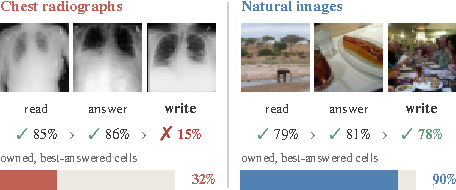
\includegraphics[width=\columnwidth]{figures/fig0_teaser.pdf}
    \caption{\textbf{Reading, answering, and ownership across image domains.} The top row shows the share of checkpoint--concept pairs that pass each RAW grade. The bars show ownership among the best-answered pairs.}
    \label{fig:teaser}
\end{figure}

Vision-language models (VLMs) can answer questions about a chest radiograph, but an accurate answer provides little information about how the model arrived at it. A linear probe, a simple classifier fitted to the model's internal image features, tests whether those features contain information about a finding.\cite{alain2017understanding,belinkov2022probing} In radiology, probes have located information about findings and detected acquisition and device cues that models could use as shortcuts.\cite{zhu2026lost,pedersen2026probes} Probes also yield a direction, a vector describing how the features would have to change to increase the probe's score for the finding.

\label{sec:related}
Activation steering changes a model's behavior by adding a vector to its internal features during prediction. Inference-time intervention and concept guidance use directions fitted by probes as steering vectors.\cite{li2023iti,vonrutte2024guide} Related steering methods use vectors derived from examples of a concept,\cite{zou2023representation,turner2023steering,panickssery2024caa} and concept activation vectors use a classifier direction to test how sensitive a prediction is to a concept.\cite{kim2018tcav} In VLMs, changing image features can alter the model's answers.\cite{rajaram2025lineofsight,ferrando2026explain} Ravichander et al.\cite{ravichander2021probing} showed that a probe can recover information the model itself does not use. Arad et al.\cite{arad2025saes} distinguished features that detect a concept from those that control an output. An audit of a clinical intervention also has to establish whether a change in the answer is specific to the labeled finding. Random vectors and a sham, a vector made by shuffling the coordinates of the fitted direction, lack a clinical label and cannot distinguish an effusion effect from one produced by another finding.

For Qwen2.5-VL-7B\cite{bai2025qwen25vl} on NIH ChestX-ray14,\cite{wang2017chestxray} adding the effusion direction increased the probability of a yes answer to the effusion question by \cfSeedWEff{}, above both random and sham controls (Fig.~\ref{fig:framework}). Adding the nodule direction on the same patients increased the effusion answer by \cfSeedWNodule{}. The effusion answer failed the ownership criterion because another finding's direction raised it more. Assessing the specificity of the effusion direction requires measuring its effects on the answers to other findings.

We developed Read--Answer--Write (RAW) to compare each finding's direction with competitors, directions fitted in the same way for other labeled concepts. RAW measures whether the model's features encode the finding, whether the model answers the question, and how its answers change when each direction is added. It applies to open-weight VLMs whose activations can be accessed. We evaluated \cfCheckpoints{} checkpoints, or saved sets of model weights, from \cfFamiliesWord{} model families on NIH ChestX-ray14 and CheXpert Plus,\cite{chambon2024chexpertplus} using COCO photographs\cite{lin2014coco} as a natural-image control.

Chest findings were readable and answerable at least as often as COCO objects, with ownership in \cfChestOwnedPct{}\% of chest pairs versus \cfCocoOwnedPct{}\% of COCO pairs (Fig.~\ref{fig:teaser}). Random and sham references alone would have certified \jnRefChest{} chest directions, half of which failed the labeled comparisons. The ownership gap persisted at comparable answer difficulty, and non-clinical attributes of the same radiographs showed similarly low ownership. Changing the components downstream of the vision tower changed ownership even when the models received the same visual features and steering directions.

\section{Materials and methods}
\label{sec:framework}
\label{app:campaign}

Read--Answer--Write (RAW) starts with a probe, a simple classifier that reads a finding from the model's image features. We then ask the model about the finding and record its answer. The probe supplies a direction, a way to change the image features so that the probe sees more evidence for the finding. We add that direction to the features and record how the model's answers change. We compare those changes with the effects of directions for other findings and with random and shuffled controls. We use these comparisons to grade how well the model represents and answers each finding, and how selectively an edit controls its answer.

\subsection{Datasets, labels and cohorts}
\label{sec:setup}
\label{app:cf-labels}
\label{app:repro-cohorts}

We used frontal radiographs from NIH ChestX-ray14 and CheXpert Plus. Both datasets label findings from radiology reports.\cite{wang2017chestxray,chambon2024chexpertplus,irvin2019chexpert} We selected frequent findings with enough positive cases. Both datasets included effusion, atelectasis, pneumothorax, and cardiomegaly. We also included mass and nodule on NIH and consolidation and edema on CheXpert Plus. The natural-image control used COCO labels for person, dog, car, chair, bottle, and bicycle.\cite{lin2014coco} We excluded uncertain or blank labels when fitting probes or scoring agreement with labels. We included those images when measuring how edits changed the model's answers.

All models used the same image lists for training, calibration, and testing. We fitted probes on the training list. We graded reading and answering on the calibration list and measured edits on the test list. The lists shared no patients or COCO images. NIH training used \cfCohortNihTrainRows{} studies from \cfCohortNihTrainUnits{} patients. Of these, \cfCohortNihTrainMulti{} contributed multiple studies, with up to \cfCohortNihTrainMax{} from one patient. All other lists used one image per patient or COCO image. CheXpert Plus and COCO each supplied \cfCohortChexTrainRows{} training images. Each dataset supplied \cfCohortNihCalibrationRows{} calibration and \cfCohortNihTestRows{} test images. Separate cohorts supplied the NIH replication images and \cfValidRows{} CheXpert films with radiologist consensus labels.\cite{irvin2019chexpert}

We selected smaller COCO objects to test the role of question difficulty. An eligible category needed at least as many positive training examples as the smallest original category. They needed at least \jnMinClassSupport{} positives in each of the calibration and test cohorts. Their mean relative area had to be below the original categories' median. We took the \jnCoreConceptCount{} categories with the most calibration positives, breaking ties by smaller area and then category identifier.

\subsection{Models and image features}
\label{app:cf-grid}

We evaluated \cfCheckpoints{} trained versions of models, called checkpoints, from \cfFamiliesWord{} general-purpose and medical families (Table~\ref{tab:cf-models}). We call each checkpoint--dataset pair a block. Each finding or object within a block is a cell. We scored about \jnScoredAnswersMillions{} million answers across \cfBlocks{} blocks and \cfCells{} cells.

The vision tower is the part of the model that encodes the image. It represents the image as lists of numbers called visual tokens. The connector prepares those tokens for the language model. We call the connector and language model together the reader. We edited the last image features that the tower sent to the connector. We also edited the connector's output to test how the language model responded when it received the edit directly. The location and selection of tokens for each model appear in Section~\ref{app:repro-sites}.

LLaVA uses CLIP,\cite{radford2021clip} which HuatuoGPT-Vision-7B retains after medical tuning. Gemma~3 uses SigLIP,\cite{zhai2023siglip} MedGemma uses medically tuned SigLIP,\cite{sellergren2025medgemma} and Qwen3-VL uses a SigLIP~2 design.\cite{tschannen2025siglip2} The chest-trained towers are XraySigLIP in CheXagent-2-3B, EVA-CLIP in CheXagent-8B, and BiomedCLIP-CXR in LLaVA-Rad-7B.\cite{chen2024chexagent,sun2023evaclip,zhang2025biomedclip,zambranochaves2025llavarad}

\begin{table*}[pos=tp]
\centering
\setlength{\tabcolsep}{3pt}
% terracotta = positive / high, blue = negative / low, sage = magnitude of Read and Ans; darker = larger magnitude
\definecolor{cfSage1}{HTML}{ECF3EF}
\definecolor{cfSage2}{HTML}{D5E5DB}
\definecolor{cfSage3}{HTML}{B9D4C3}
\definecolor{cfSage4}{HTML}{9EC3AC}
\definecolor{cfSlate1}{HTML}{EAF0F6}
\definecolor{cfSlate2}{HTML}{D0DDEA}
\definecolor{cfSlate3}{HTML}{B1C7DD}
\definecolor{cfSlate4}{HTML}{94B2D0}
\definecolor{cfTerra1}{HTML}{F7ECEA}
\definecolor{cfTerra2}{HTML}{EED5D1}
\definecolor{cfTerra3}{HTML}{E2B8B2}
\definecolor{cfTerra4}{HTML}{D79E95}
\definecolor{cfOat1}{HTML}{F4EFE6}
\definecolor{cfOat2}{HTML}{E8DDC8}
\definecolor{cfGrey}{HTML}{E4E1DC}

\caption{\textbf{Checkpoints and families.} Checkpoint rows give the vision tower, visual tokens passed to the connector per image, input size, and eligible templates. Bold family rows give mean selectivity and clean-answer AUROC over clinical cells, then the owned clinical and COCO cells, shaded by owned share.}
\label{tab:cf-models}
\fitwidth{%
\cftabsize
\begin{tabular}{lllll@{\hspace{8pt}}rrrr}
\toprule
\multirow{2}{*}{Checkpoint} & \multirow{2}{*}{Vision tower} & \multirow{2}{*}{Tokens} & \multirow{2}{*}{Image} & \multirow{2}{*}{Templates} & \multirow{2}{*}{$\bar S$} & \multirow{2}{*}{$\overline{\mathrm{AUROC}}$} & \multicolumn{2}{c}{owned cells}\\
\cmidrule(lr){8-9}
&  &  &  &  &  &  & \multicolumn{1}{c}{clinical} & \multicolumn{1}{c}{COCO}\\
\midrule
\multicolumn{5}{l}{\textbf{Qwen2.5-VL}\cite{bai2025qwen25vl}} & 0.132 & 0.635 & \cellcolor{cfTerra2}5/48 & \cellcolor{cfTerra4}24/24 \\
\quad Qwen2.5-VL-3B & native ViT 675M & 576$\to$144 & $336^2$ & IYWYIAWA & & & & \\
\quad Qwen2.5-VL-7B & native ViT 675M & 576$\to$144 & $336^2$ & all & & & & \\
\quad Qwen2.5-VL-32B & native ViT 675M & 576$\to$144 & $336^2$ & all & & & & \\
\quad Qwen2.5-VL-72B & native ViT 675M & 576$\to$144 & $336^2$ & all & & & & \\
\midrule
\multicolumn{5}{l}{\textbf{Qwen3-VL}\cite{qwen2025qwen3vl}} & 0.137 & 0.735 & \cellcolor{cfTerra3}6/36 & \cellcolor{cfTerra4}18/18 \\
\quad Qwen3-VL-4B & SigLIP2-based & $\leq$1024 & $\leq 512^2$ & all & & & & \\
\quad Qwen3-VL-8B & SigLIP2-based & $\leq$1024 & $\leq 512^2$ & all & & & & \\
\quad Qwen3-VL-32B & SigLIP2-based & $\leq$1024 & $\leq 512^2$ & all & & & & \\
\midrule
\multicolumn{5}{l}{\textbf{InternVL3.5}\cite{wang2025internvl35}} & 0.125 & 0.807 & \cellcolor{cfTerra3}6/36 & \cellcolor{cfTerra4}18/18 \\
\quad InternVL3.5-8B & InternViT-300M & 1024 & $448^2$ & all & & & & \\
\quad InternVL3.5-14B & InternViT-300M & 1024 & $448^2$ & all & & & & \\
\quad InternVL3.5-38B & InternViT-6B & 1024 & $448^2$ & all & & & & \\
\midrule
\multicolumn{5}{l}{\textbf{Gemma 3}\cite{gemma2025gemma3}} & 0.124 & 0.564 & \cellcolor{cfTerra2}4/36 & \cellcolor{cfTerra4}17/18 \\
\quad Gemma 3 4B & SigLIP-So400m & 4096 & $896^2$ & all & & & & \\
\quad Gemma 3 12B & SigLIP-So400m & 4096 & $896^2$ & all & & & & \\
\quad Gemma 3 27B & SigLIP-So400m & 4096 & $896^2$ & all & & & & \\
\midrule
\multicolumn{5}{l}{\textbf{MedGemma} (medical)\cite{sellergren2025medgemma}} & 0.164 & 0.835 & \cellcolor{cfTerra2}2/24 & \cellcolor{cfTerra3}10/12 \\
\quad MedGemma 4B & MedSigLIP & 4096 & $896^2$ & all & & & & \\
\quad MedGemma 27B & MedSigLIP & 4096 & $896^2$ & all & & & & \\
\midrule
\multicolumn{5}{l}{\textbf{Lingshu} (medical)\cite{lasa2025lingshu}} & 0.142 & 0.820 & \cellcolor{cfTerra4}12/24 & \cellcolor{cfTerra4}12/12 \\
\quad Lingshu 7B & Qwen2.5-VL ViT & 576$\to$144 & $336^2$ & all & & & & \\
\quad Lingshu 32B & Qwen2.5-VL ViT & 576$\to$144 & $336^2$ & all & & & & \\
\midrule
\multicolumn{5}{l}{\textbf{LLaVA-1.5}\cite{liu2024improved}} & 0.124 & 0.516 & \cellcolor{cfTerra1}0/24 & \cellcolor{cfTerra3}8/12 \\
\quad LLaVA-1.5-7B & CLIP ViT-L/14-336 & 576 & $336^2$ & IYWY & & & & \\
\quad LLaVA-1.5-13B & CLIP ViT-L/14-336 & 576 & $336^2$ & IYWYIAWA & & & & \\
\midrule
\multicolumn{5}{l}{\textbf{LLaVA-Med} (medical)\cite{li2023llavamed}} & 0.136 & 0.560 & \cellcolor{cfTerra2}1/12 & \cellcolor{cfTerra2}1/6 \\
\quad LLaVA-Med 1.5 7B & CLIP ViT-L/14-336 & 576 & $336^2$ & IYWY & & & & \\
\midrule
\multicolumn{5}{l}{\textbf{Llama 3.2 Vision}\cite{meta2024llama32vision}} & 0.119 & 0.688 & \cellcolor{cfTerra1}0/12 & \cellcolor{cfTerra2}1/6 \\
\quad Llama 3.2 Vision 11B & ViT-H/14 & 1601 & $560^2$ & IBWB & & & & \\
\midrule
\multicolumn{5}{l}{\textbf{CheXagent} (medical)\cite{chen2024chexagent}} & 0.180 & 0.857 & \cellcolor{cfTerra3}7/24 & \cellcolor{cfTerra2}2/12 \\
\quad CheXagent-2-3B & XraySigLIP ViT-L/16 & 1024 & $512^2$ & IYWYIAWA & & & & \\
\quad CheXagent-8B & EVA-CLIP ViT 1.4B & 1025$\to$128 & $448^2$ & IYWYIAWA & & & & \\
\midrule
\multicolumn{5}{l}{\textbf{LLaVA-Rad} (medical)\cite{zambranochaves2025llavarad}} & 0.209 & 0.793 & \cellcolor{cfTerra1}0/12 & \cellcolor{cfTerra1}0/6 \\
\quad LLaVA-Rad-7B & BiomedCLIP-CXR-518 & 1369 & $518^2$ & IYWY & & & & \\
\midrule
\multicolumn{5}{l}{\textbf{HuatuoGPT-Vision} (medical)\cite{chen2024huatuogptvision}} & 0.136 & 0.746 & \cellcolor{cfTerra2}1/12 & \cellcolor{cfTerra4}6/6 \\
\quad HuatuoGPT-Vision-7B & CLIP ViT-L/14-336 & 576 & $336^2$ & all & & & & \\
\bottomrule
\end{tabular}}
\end{table*}


\subsection{Reading and writing findings}
\label{sec:site}

\begin{figure*}[pos=tp]
    \centering
    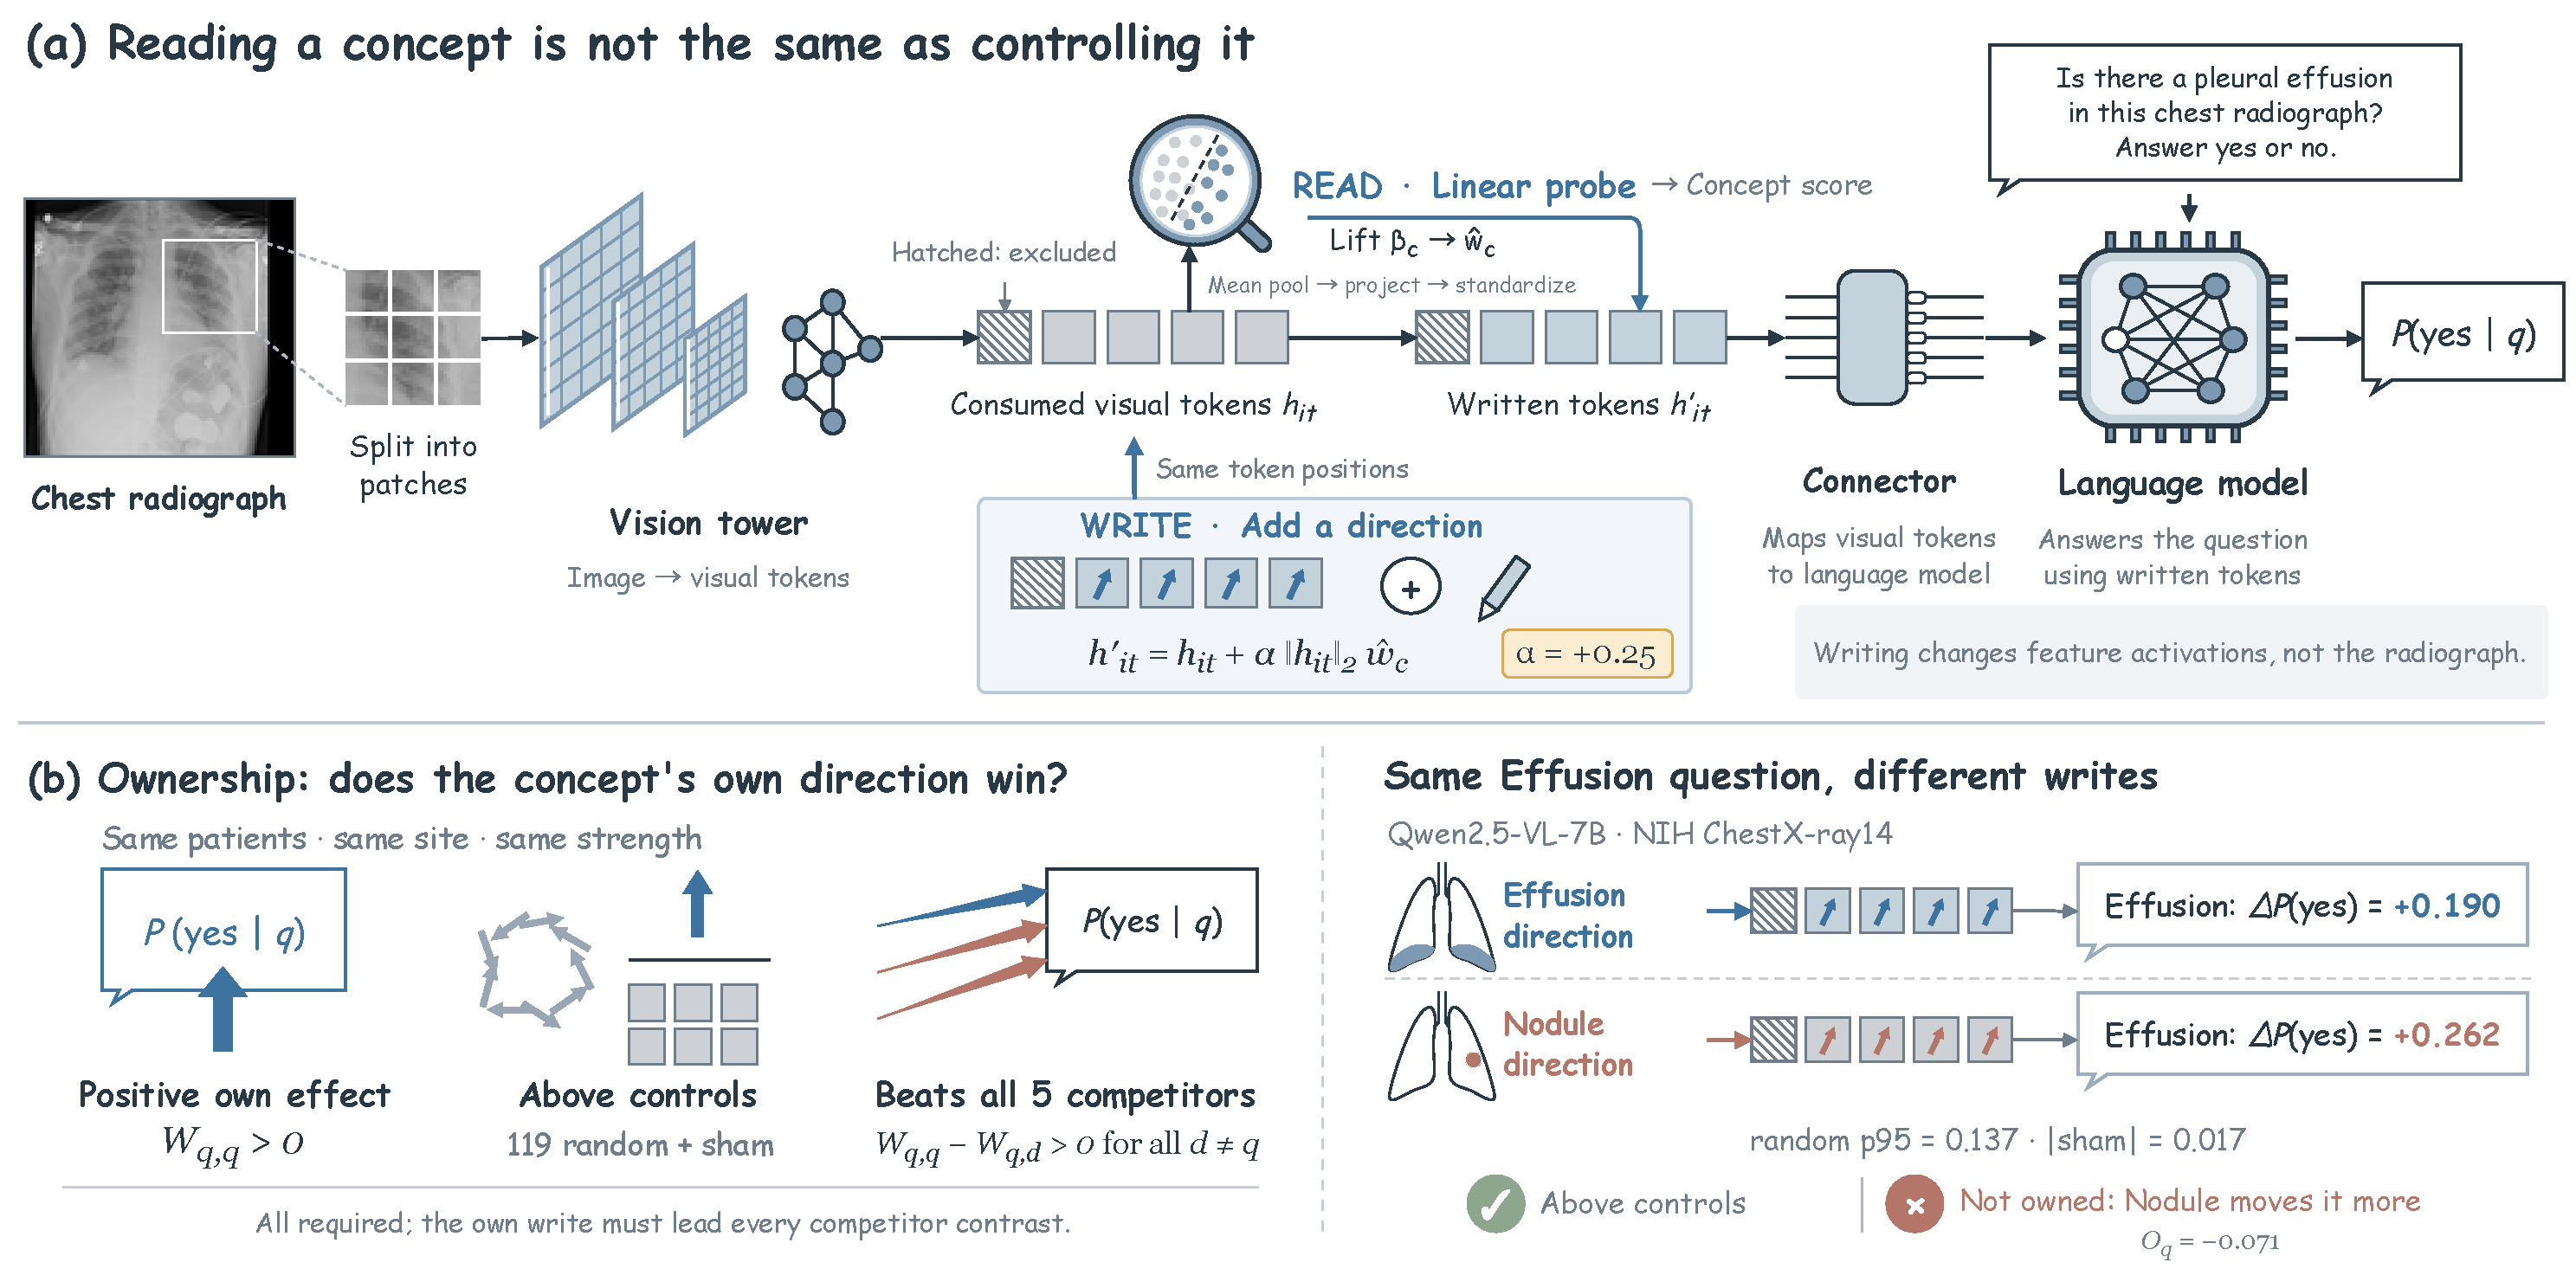
\includegraphics[width=\linewidth]{figures/fig1_framework.pdf}
    \caption{\textbf{Reading and writing at the selected vision layer.} (a) The probe reads the visual tokens that receive the write. Hatching marks token positions the connector excludes. (b) On NIH ChestX-ray14, the nodule write raises Qwen2.5-VL-7B's effusion answer more than the effusion write does.}
    \label{fig:framework}
\end{figure*}

For each image, we averaged the tokens from the selected layer. We reduced the number of features and put them on a common scale using the training images. We fitted a logistic regression probe to predict whether each finding was present. The \emph{label direction} is the change in the original image features that most increases the probe score per unit of change (Eq.~\ref{eq:lift}).

A write adds the direction to the tokens the probe read (Fig.~\ref{fig:framework}). To compare edits across models, we set the \emph{steering strength} relative to each token's length. The main edit used a fraction of \jnPrimaryStrength{} to move toward higher probe scores. We also tested other strengths (Section~\ref{sec:write-implementation}).

\subsection{Controls for reading and writing}
\label{sec:directions}

We measured probe performance with the area under the receiver operating characteristic curve (AUROC). It estimates the chance that a positive example scores higher than a negative example, with half credit for ties. We compared the probe's AUROC with that of probes trained on randomly assigned labels. Images of the same type shared a random label. On chest radiographs we grouped images by projection, recorded sex, and age decade. On COCO we used aspect ratio and area. The concept probe's AUROC minus the mean AUROC of valid random-label probes is its \emph{selectivity}, denoted by $S$ (Eq.~\ref{eq:selectivity}).

A \emph{competitor} is a direction fitted to another finding or object. We also drew \jnRandomDirections{} random directions. A \emph{sham} shuffles the values of the target direction. All controls used the same strength and images as the target direction.

\subsection{Questions and scoring}
\label{app:protocol}

The questions used \emph{is there} (I) or \emph{does the image show} (W). Both wordings used yes/no (Y) and two letter mappings (A-present and B-present). The primary prompt was IY. When yes/no failed the answer mapping check, we graded a valid letter-coded prompt (Section~\ref{app:cf-gates}).

For each question we measured the model's support for yes relative to no at the first answer position. We write this score as $P(\mathrm{yes})$. The \emph{clean answer} is the score before an edit. We also used the \emph{answer margin}, the difference between the log probabilities of yes and no before conversion to a score (Section~\ref{sec:scoring-implementation}). Tables~\ref{tab:key-terms} and \ref{tab:notation} summarize the terms and symbols.

\begin{table}[pos=b]
\centering
\caption{\textbf{Key terms.} Definitions for the RAW evaluation.}
\label{tab:key-terms}
\fitwidth{%
\cftabsize
\begin{tabular}{@{}lp{0.70\columnwidth}@{}}
\toprule
Term & Definition \\
\midrule
Probe & Classifier fitted to the model's image features. \\
Direction & Vector specifying how features change. \\
Write & Addition of a direction to the features. \\
Reader & Connector and language model. \\
Competitor & Direction fitted for another labeled concept. \\
Sham & Control made by shuffling a direction's coordinates. \\
Cell & One checkpoint and one concept on a dataset. \\
Block & One checkpoint evaluated on one dataset. \\
\bottomrule
\end{tabular}}
\end{table}

\begin{table*}[pos=tp]
\centering
\caption{\textbf{Notation used in the study.} Symbols for features, answers, and effects of edits.}
\label{tab:notation}
\fitwidth{%
\cftabsize
\begin{tabular}{@{}lp{0.80\linewidth}@{}}
\toprule
Symbol & Definition \\
\midrule
$c$, $q$, $d$ & Concept, question about a concept, and direction fitted for a concept. \\
$\hvec_{it}$, $\hvec_i$ & Visual token $t$ of image $i$ and the mean of its selected tokens. \\
$D$, $R$, $\boldsymbol s$, $\boldsymbol\beta_c$ & Vision feature dimension, Gaussian projection, training feature scales, and probe coefficients. \\
$\hat\wvec_c$, $a_q$ & Directions fitted to labels (Eq.~\ref{eq:lift}) and to clean answers (Eq.~\ref{eq:answer-direction}). \\
$\alpha$, $S$ & Signed edit strength relative to token length and probe selectivity (Eq.~\ref{eq:selectivity}). \\
$W_{q,d}$ & Mean change in question $q$'s score under direction $d$. \\
$O_q$, $C_d$ & Row and column margins (Eqs.~\ref{eq:margin} and \ref{eq:column-margin}). \\
$O_q^m$ & Row margin calculated from changes in the log-probability difference for yes versus no. \\
$\kappa_d$ & Signed own effect divided by total absolute change (Eq.~\ref{eq:column-selectivity}). \\
$F_{q,d}$ & Mean positive change over checkpoints, shown by band width in Fig.~\ref{fig:write-flow}. \\
$\cos_\Sigma$ & Cosine weighted by training-feature covariance $\Sigma$ (Eq.~\ref{eq:whitened-cos}). \\
\bottomrule
\end{tabular}}
\end{table*}

\subsection{Ownership and direction specificity}
\label{sec:ownership}

The write matrix has one row per question and one column per direction. Entry $W_{q,d}$ is the mean change to answer $q$ when we add direction $d$ on the same test images. The diagonal entry $W_{q,q}$ is the \emph{own write}. It meets the steering reference if the increase exceeds the ninety-fifth percentile of random effects and the absolute sham effect.

\emph{Ownership} asks which direction raises a given answer the most. The row margin $O_q$ subtracts the largest competing effect from the own write.
\begin{equation}
O_q=W_{q,q}-\max_{d\ne q}W_{q,d}.
\label{eq:margin}
\end{equation}
A cell is owned when it meets the steering reference and this margin is positive.

\emph{Direction specificity} asks which answer changes most under a given direction. The column margin $C_d$ subtracts the largest absolute change on any other answer from the own write.
\begin{equation}
C_d=W_{d,d}-\max_{q\ne d}\lvert W_{q,d}\rvert.
\label{eq:column-margin}
\end{equation}
A cell is specific when it meets the reference and this margin is positive. A large decrease in another answer counts against specificity. We report total absolute change in other answers relative to the own write. \emph{Column selectivity} $\kappa_d$ measures the share attributable to the signed own write.
\begin{equation}
\kappa_d=\frac{W_{d,d}}{\sum_q\lvert W_{q,d}\rvert}.
\label{eq:column-selectivity}
\end{equation}
It equals one if the edit raises only its own answer and leaves the others unchanged.

\subsection{Decision rules and supporting analyses}
\label{sec:grades}

\begin{table}[pos=t]
\centering
\caption{\textbf{RAW grades.} Reading and answering use calibration data. Intervention criteria use the test cohort.}
\label{tab:grades}
\fitwidth{%
\cftabsize
\begin{tabular}{@{}lp{0.62\columnwidth}@{}}
\toprule
Grade & Criterion \\
\midrule
Readable & Probe selectivity $S>0$ \\
Answerable & Clean-answer AUROC above chance \\
Owned & Steering reference met and $O_q>0$ \\
Specific & Steering reference met and $C_d>0$ \\
Owned and specific & Steering reference met, $O_q>0$ and $C_d>0$ \\
\bottomrule
\end{tabular}}
\end{table}

To grade readability or answerability, we required at least \jnMinClassSupport{} known positives and \jnMinClassSupport{} known negatives in the calibration group. Readability also required a valid AUROC for the finding probe and at least \jnMinValidControls{} valid control AUROCs. Table~\ref{tab:grades} gives the criteria. To assess sensitivity to the choice of competitors, we repeated the comparison for every subset of a given size and averaged the owned counts.

We compared alternative directions and tested edits concentrated on high-scoring tokens. We regraded changes on the answer-margin scale, using $O_q^m$ for its row margin. We repeated grading on images with a clean yes score between \jnSaturationLow{} and \jnSaturationHigh{}, and grouped results by clean answer and label. We checked the grades against radiologist consensus and applied directions fitted to those labels to the main test cohort. For comparison, we fitted directions to report labels from the same films, size-matched training subsets, and the full training set.

\label{app:cf-difficulty}
We graded the smaller COCO objects on the same checkpoints and images as the original objects. We pooled both COCO sets and grouped cells by clean-answer AUROC at \cfStratEdges{}. We also compared cells at minimum AUROCs of \jnCsAurocLower{} and \jnCsAurocHigher{}, where the domains overlapped more. A logistic model predicted ownership from image domain, AUROC, and probe selectivity. For each cell we predicted ownership under both domains at its observed AUROC and selectivity. We averaged the differences between those predictions. For the adjusted results and highest AUROC group, we estimated standard deviations from \jnBootstrapResamples{} resamples of whole checkpoints with replacement.

We also graded directions for projection (anteroposterior or portable versus posteroanterior), recorded sex, and age at least \jnAttributeAgeCutoff{} years. The attributes and findings competed in \cfAttrRefBlocks{} blocks under the same controls. Calibration tried \cfAttrqPhrasings{} wordings per attribute. We compared all cells, answerable cells, and cells matched within \cfAttrPairWindow{} clean-answer AUROC in the same block.

To test the reader's role, we paired the Gemma~3 4B and MedGemma 4B towers with both readers. Directions stayed with the towers. We also gave readers from shared-tower checkpoints the same stored features and edits (Section~\ref{app:cf-crossed-reader}).

We fitted an \emph{answer direction} to unedited answers. We compared its alignment and agreement with labels against the label direction. We also tested negated questions and choices between the finding and its strongest competitor, in both orders. A further test scored the finding word in a report continuation (Section~\ref{sec:scoring-implementation}).

\subsection{Registration and reproducibility}
\label{app:repro}
\label{app:repro-protocol}

We registered the layers, settings, controls, prompts, and rules before scoring. Dated amendments preceded the additional analyses, including category selection and difficulty comparisons. Rankings, changes across answers, and individual examples describe the completed runs. The release includes code, adapters, protocol, cohort lists and seeds, directions, image-level results, scorecards, and prompts.

\subsubsection{Registered NIH replication and prompt experiments}
\label{app:seed}

The NIH experiments used LLaVA-1.5-7B for effusion and edema and Qwen2.5-VL-7B for effusion.\cite{liu2024improved,bai2025qwen25vl} We assigned patients to separate training, validation, and test groups by hashing their identifiers. Training used \jnReplicationTrainingRows{} images. The held-out group included \jnReplicationTestRows{} images from \jnReplicationTestPatients{} patients. We verified that the write reached the answer scores and that zero strength reproduced the clean answer. Selectivity used \jnLabelControlCount{} random-label maps over \jnReplicationLabelTypes{} image types.

We tested the initial writes across several strengths on \jnReplicationInitialRows{} images (Section~\ref{sec:write-implementation}). Controls included \jnLabelControlCount{} random directions, the sham, and the fixed competitors. For the strengths in $\mathcal A=\jnReplicationControlStrengths$, we picked the strength $\alpha_c^\star$ that gave the largest change in the intended direction. Here $\Delta_c(\alpha)$ is the mean change from the clean score for concept $c$ at strength $\alpha$, and $\Delta_c^\star$ is the selected signed change.
\begin{equation}
\begin{aligned}
\alpha_c^\star &=
  \operatorname*{arg\,max}_{\alpha\in\mathcal A}
  \operatorname{sign}(\alpha)\Delta_c(\alpha),\\
\Delta_c^\star &=\operatorname{sign}(\alpha_c^\star)
                 \Delta_c(\alpha_c^\star).
\end{aligned}
\label{eq:seed-rule}
\end{equation}
We compared the selected change with the largest absolute sham effect across controlled strengths and the ninety-fifth percentile of signed random effects at the selected strength. We described how steadily the scores moved over $\jnStrengthSweepBounds$.

At the primary strength we tested one image from each of \jnReplicationEffusionRows{} new patients selected by label-blind hash. With \jnLabelControlCount{} random directions, a sham, and clinical competitors, this gave \jnReplicationConfigurations{} conditions and \jnReplicationOutcomeCount{} image-level outcomes. The own write had to exceed the random cutoff, sham effect, and competitors. We then tested all findings in \jnReplicationMatrixRows{} new patients using the largest random effect as the cutoff. We measured each direction's mean signed effect on other answers and its excess over their own writes.

The letter-mapping test used \jnReplicationPromptRows{} patients and an equally sized, distinct calibration group. Eligibility required above-chance AUROC under both mappings and \jnMinClassSupport{} patients per class. Edits at $\jnReplicationPromptStrengths$ used \jnLabelControlCount{} random directions and a sham. The mass confirmation used both wordings and all formats in \jnReplicationMassRows{} further patients. The primary write had to beat \jnLabelControlCount{} clinical comparisons, the largest of \jnRandomDirections{} random effects, and the absolute sham effect in all letter conditions or both yes/no conditions (Section~\ref{app:seed-results}).

\subsection{Implementation details}
\label{sec:implementation}

\subsubsection{Vision layers and token selection}
\label{app:repro-sites}
\label{app:repro-mask}

Models ran in bfloat16 with their native processors and fixed resolutions. Processor outputs identified the \cfTokensMin{} to \cfTokensMax{} tokens selected per image.

\begin{itemize}[leftmargin=*,itemsep=1pt,topsep=2pt]
\item Qwen2.5-VL and Lingshu used the last of \jnQwenVisionDepth{} blocks. Qwen3-VL used the last of \jnQwenThreeShallowDepth{} at 4B or \jnQwenThreeDeepDepth{} at 8B and 32B. The patch grid identified each image's contiguous span. The connector merged $\jnPatchGroupSide\times\jnPatchGroupSide$ patches. Earlier DeepStack branches bypassed the edit.
\item Gemma~3 and MedGemma used all normalized patches from the last of \jnSiglipDepth{} SigLIP layers. InternVL3.5 used the last of \jnInternVlShallowDepth{} InternViT layers at 8B and 14B, or \jnInternVlDeepDepth{} at 38B. Its final normalization was an identity. We kept patch tokens from the single tile and excluded its image-summary token (CLS). Patch counts had to match image placeholders.
\item LLaVA-1.5 and LLaVA-Med used the penultimate of \jnClipDepth{} CLIP layers and excluded CLS. Llama~3.2 Vision used the last of \jnLlamaGlobalDepth{} global layers. Its \jnLlamaLocalBranches{} intermediate local inputs bypassed the edit. We kept CLS and the patches of the real tile and excluded its \jnLlamaPaddingTokens{} padding tokens and the \jnLlamaPaddingTiles{} padded tiles.
\end{itemize}

We rejected incomplete spans, mask mismatches, empty images, and repeated calls to the layer in one pass. Records identify the layer, feature dimension, connector, and bypassed branches.

\subsubsection{Probe fitting and control generation}
\label{app:repro-probe}
\label{app:repro-controls}

For image $i$, $\hvec_i$ is its mean selected token vector. Projection matrix $R$ has $D$ original feature rows and $m=\cfAltdirdGramDim$ projected columns. PCG64 with seed zero drew independent standard normal entries. We divided by $\sqrt{m}$ and stored in single precision. We centered features at their training means and scaled by their standard deviations, floored at $\jnScaleFloor$. The $\ell_2$-regularized fit used unweighted classes, inverse penalty $C=1$, and up to \jnProbeMaxIterations{} L-BFGS iterations. Refits resampled whole patients or images with replacement and refitted scales and probes with the same projection and control seeds.

To express the fitted direction in the original features, we divide the probe coefficients $\boldsymbol\beta_c$ for finding $c$ by the feature scales $\boldsymbol s$. We map the result back with $R$ to give $\boldsymbol g_c$, then normalize it to unit length to obtain $\hat\wvec_c$.
\begin{equation}
\begin{aligned}
\boldsymbol g_c &= R\,\mathrm{diag}(\boldsymbol s)^{-1}\boldsymbol\beta_c,\\
\hat\wvec_c &= \boldsymbol g_c/\lVert\boldsymbol g_c\rVert_2.
\end{aligned}
\label{eq:lift}
\end{equation}

For the \jnLabelControlCount{} random-label probes we used successive PCG64 seeds starting at zero. We drew equiprobable binary labels for image types in sorted order. If all types received the same label, we flipped the first. We fitted the controls using the same known-label rows and settings as the finding probe. Fitting controls required at least \jnMinControlTypes{} types per block. With labels $y$, probe scores $r$, and $K$ valid controls, selectivity is
\begin{equation}
S=\operatorname{AUROC}(y,r)-
\frac{1}{K}\sum_{k=1}^{K}\operatorname{AUROC}
             (y_k^{\mathrm{ctrl}},r_k^{\mathrm{ctrl}}).
\label{eq:selectivity}
\end{equation}
The subscript $k$ identifies the control and the superscript $\mathrm{ctrl}$ distinguishes its labels and scores.

For the write controls, PCG64 with seed zero drew Gaussian vectors. We normalized each vector to unit length and shared the draws across questions within a block. The same generator produced one coordinate permutation per label direction in protocol order for the shams.

\subsubsection{Writes and alternative directions}
\label{sec:write-implementation}

For token $t$ of image $i$, $\hvec_{it}$ is the original feature vector and $\hvec'_{it}$ is the edited vector. We add the unit direction for finding $c$ after scaling it by the token length and signed steering strength $\alpha$.
\begin{equation}
\hvec'_{it}=\hvec_{it}+\alpha\lVert\hvec_{it}\rVert_2\,\hat\wvec_c.
\label{eq:intervention}
\end{equation}
The main write used $\alpha=\jnPrimaryStrength$. The sweep also tested $\alpha\in\jnOtherStrengths$. The NIH replication used
\[\alpha\in\jnReplicationStrengths.\]

We compared the probe direction with the difference between positive and negative feature means and the activation pattern associated with the probe weights (Haufe pattern).\cite{haufe2014interpretation} Other variants projected the probe away from the competing directions or refitted it after removing the linear contribution of the competing labels. For a direct change $\boldsymbol u$ in the projected and scaled features, we used the shortest corresponding vector in the original features, up to scale.
\begin{equation}
\begin{aligned}
\hat\wvec &\propto R(R^{\top}R)^{-1}
             \mathrm{diag}(\boldsymbol s)\,\boldsymbol u,\\
R^\top\hat\wvec &\propto \mathrm{diag}(\boldsymbol s)\,\boldsymbol u .
\end{aligned}
\label{eq:displacement-lift}
\end{equation}
This conversion differs from the coefficient conversion because $R^\top R$ is not proportional to the identity. The matrix $R^\top R/D$ had full rank $m$ in the \cfAltdirdBlocks{} blocks tested. Its eigenvalues ranged from $\cfAltdirdEigMin$ to $\cfAltdirdEigMax$. Its condition numbers ranged from \cfAltdirdCondMin{} to \cfAltdirdCondMax{}.

We also varied the write across tokens. Each weight $\omega_t$ depends on the token's probe score $z_t$. For $n_{\mathrm{tok}}$ selected tokens, the weights average one. One variant weighted scores by their exponentials (softmax). Another wrote only to the highest-scoring quarter.
\begin{equation}
\begin{aligned}
\hvec'_{it}&=\hvec_{it}+\alpha\omega_t\lVert\hvec_{it}\rVert_2\,\hat\wvec_c,\\
\omega_t^{\mathrm{softmax}}
  &=n_{\mathrm{tok}}e^{z_t}\big/\sum_{t'}e^{z_{t'}},\\
\omega_t^{\mathrm{quarter}}
  &=4\,\mathbf 1[\,z_t\in\text{top quarter}\,].
\end{aligned}
\label{eq:token-weights}
\end{equation}
Here $t'$ ranges over selected tokens and $\mathbf 1$ is one for selected high-scoring tokens and zero otherwise. The softmax kept the sum of weights fixed. The top-quarter variant doubled their Euclidean norm. Extended comparisons added directions for labels with at least \jnMinExtendedClassSupport{} known positives and negatives. These were consolidation, edema, and infiltration on NIH, and enlarged cardiomediastinum, fracture, lung lesion, lung opacity, pneumonia, and support devices on CheXpert Plus.

\subsubsection{Acceptance checks and coverage}
\label{sec:gates}
\label{app:cf-gates}
\label{app:cf-coverage}

We used \cfCohortNihPreflightRows{} images at both sites. Checks covered repeatability (A), zero-strength identity (B), and whether the first concept's primary write changed downstream scores within the token mask (C). We compared batched and single-image passes (D) and tested answer mappings without images (E). We checked throughput (F) and recomputed scores at single precision (G). Each question used fixed image groups across conditions. Eligible prompts passed the mapping check. All \cfWriteBlocks{} completed blocks passed A--C, and single-precision differences were below \cfGateFpMax{}. We rescored the first \jnPrecisionRows{} test rows singly at single precision.

The \cfCoveragePlannedWord{} planned components were the core write matrix and calibration, additional prompts, the strength sweep, probe refits, and writes and calibration at the connector output. All \cfBlocks{} blocks completed the core matrix and calibration. Of these, \cfCoverageBlocksAllSeven{} completed all components. The Qwen2.5-VL-72B CheXpert Plus block lacked the extra prompts and connector tests. A successful probe with an ineligible or incomplete matrix contributed only readability. Scorecards retain the range over $\jnStrengthSweepBounds$, refit standard deviations, connector-output grades, and prompt comparisons. The study used about \jnEvaluationComputeHours{} A100 GPU-hours. A chest block from a model with seven billion parameters took about \jnChestBlockHours{} hours.

\subsubsection{Reader swaps and feature replay}
\label{app:cf-crossed-reader}

In the crossed experiment, the swapped tower matched \cfSwapTensors{} donor weight arrays exactly. The \cfSwapOutside{} arrays outside the tower were unchanged. All combinations used the same \cfSwapRows{} test images, primary strength and prompt, and the controls for the installed tower. Let $Y_q(g/h)$ be the measurement for question $q$ with tower $g$ and reader $h$. The model identifiers $\mathrm G$ and $\mathrm M$ denote Gemma~3 and MedGemma.
\begin{equation}
\begin{aligned}
\delta_{\text{reader}}&=\tfrac{1}{12}\sum_{g,q}
  \lvert Y_q(g/\mathrm G)-Y_q(g/\mathrm M)\rvert,\\
\delta_{\text{tower}}&=\tfrac{1}{12}\sum_{h,q}
  \lvert Y_q(\mathrm G/h)-Y_q(\mathrm M/h)\rvert.
\end{aligned}
\label{eq:crossover}
\end{equation}
The two effects average absolute changes after replacing either the reader or the tower. Measurements were the own write $W_{q,q}$, the row margin $O_q$, and the margin over the largest competing, random-cutoff, or absolute sham effect, denoted by $M_q$. For the replay, we stored the selected tokens from one checkpoint and used them in place of both checkpoints' own features. We first measured how much the stored and original tokens differed. Replaying a checkpoint's own tokens checked the substitution path.

\subsubsection{Answer scores, answer directions, and other response formats}
\label{sec:scoring-implementation}

For each answer we used the highest log probability among its valid single-token forms, including case and leading spaces. Let $\ell_{\mathrm{yes}}$ and $\ell_{\mathrm{no}}$ be those log probabilities. We calculated the yes score as $P(\mathrm{yes})=\sigma(\ell_{\mathrm{yes}}-\ell_{\mathrm{no}})$, where $\sigma$ is the logistic function.

The answer direction $a_q$ uses ridge regression of the clean margin $m_{iq}$ on standardized features $\boldsymbol x_i$ for image $i$ and question $q$. Ridge regression penalizes large coefficients. The fit uses intercept $\gamma_0$, coefficients $\boldsymbol\gamma$, and penalty $\lambda$.
\begin{equation}
\begin{split}
\boldsymbol\gamma_q=\arg\min_{\gamma_0,\boldsymbol\gamma}\;\bigg[
 &\sum_i (m_{iq}-\gamma_0-\boldsymbol x_i^\top\boldsymbol\gamma)^2\\
 &+\lambda\lVert\boldsymbol\gamma\rVert_2^2\bigg].
\end{split}
\label{eq:answer-direction}
\end{equation}
We used the first \jnAnswerDirectionFitRows{} training images in label-blind order. We chose $\lambda\in\jnRidgePenalties$ by five-fold cross-validation over patients or images to maximize $R^2$. We converted coefficients by Eq.~\ref{eq:lift}. The controls were other answer directions, random directions, and a sham. New prompts used the same direction with their own clean score and sham.

The cosine measures how closely two directions align. We also measured a version that accounts for how much the training features vary together.\cite{park2024linear} Let $\Sigma$ be the training-feature covariance and $\boldsymbol\beta$ and $\boldsymbol\beta'$ be two sets of projected coefficients. The covariance-weighted cosine is the correlation of their scores on training images.
\begin{equation}
\cos_\Sigma(\boldsymbol\beta,\boldsymbol\beta')
=\frac{\boldsymbol\beta^\top\Sigma\boldsymbol\beta'}
{\sqrt{(\boldsymbol\beta^\top\Sigma\boldsymbol\beta)
        (\boldsymbol\beta'^\top\Sigma\boldsymbol\beta')}}.
\label{eq:whitened-cos}
\end{equation}

The negated question should move in the opposite direction to the original. For the report continuation we scored the log probability of the finding word. Each format used its own clean score, sham, and \cfSemLedgerRandom{} random directions. The signed effect $E_q$ met the reference if it exceeded zero, the largest random effect $E_k^{\mathrm{rand}}$, and the absolute sham effect.
\begin{equation}
E_q>\max\bigl(0,\;\max_k E_k^{\mathrm{rand}},\;
                   \lvert E_q^{\mathrm{sham}}\rvert\bigr).
\label{eq:endpoint-reference}
\end{equation}
Ownership also required a larger effect than the labeled competitors on the same question.

\section{Results}
\label{sec:results}

\begin{table*}[pos=t]
\centering
\setlength{\tabcolsep}{3pt}
\renewcommand{\arraystretch}{1.08}
% terracotta = positive / high, blue = negative / low, sage = magnitude of Read and Ans; darker = larger magnitude
\definecolor{cfSage1}{HTML}{ECF3EF}
\definecolor{cfSage2}{HTML}{D5E5DB}
\definecolor{cfSage3}{HTML}{B9D4C3}
\definecolor{cfSage4}{HTML}{9EC3AC}
\definecolor{cfSlate1}{HTML}{EAF0F6}
\definecolor{cfSlate2}{HTML}{D0DDEA}
\definecolor{cfSlate3}{HTML}{B1C7DD}
\definecolor{cfSlate4}{HTML}{94B2D0}
\definecolor{cfTerra1}{HTML}{F7ECEA}
\definecolor{cfTerra2}{HTML}{EED5D1}
\definecolor{cfTerra3}{HTML}{E2B8B2}
\definecolor{cfTerra4}{HTML}{D79E95}
\definecolor{cfOat1}{HTML}{F4EFE6}
\definecolor{cfOat2}{HTML}{E8DDC8}
\definecolor{cfGrey}{HTML}{E4E1DC}

\caption{\textbf{RAW grades by checkpoint and dataset.} Read, Ans, and Own give mean probe selectivity, clean-answer AUROC, and row margin. Superscripts count concepts meeting each grade. The final columns give the owned share for chest radiographs and COCO and their ratio. Blue indicates a negative row margin.}
\label{tab:cf-main}
\fitwidth{%
\cftabsize
\begin{tabular}{l@{\hspace{7pt}}ccc@{\hspace{4pt}}ccc@{\hspace{4pt}}ccc@{\hspace{4pt}}ccc}
\toprule
\multirow{2}{*}{Checkpoint} & \multicolumn{3}{c}{NIH ChestX-ray14} & \multicolumn{3}{c}{CheXpert Plus} & \multicolumn{3}{c}{COCO (control)} & \multicolumn{3}{c}{Owned share}\\
\cmidrule(lr){2-4}\cmidrule(lr){5-7}\cmidrule(lr){8-10}\cmidrule(lr){11-13}
& \multicolumn{1}{c}{Read} & \multicolumn{1}{c}{Ans} & \multicolumn{1}{c}{Own} & \multicolumn{1}{c}{Read} & \multicolumn{1}{c}{Ans} & \multicolumn{1}{c}{Own} & \multicolumn{1}{c}{Read} & \multicolumn{1}{c}{Ans} & \multicolumn{1}{c}{Own} & \multicolumn{1}{c}{clin.} & \multicolumn{1}{c}{COCO} & \multicolumn{1}{c}{ratio}\\
\midrule
Lingshu 32B & \cellcolor{cfSage2}0.08$^{5}$ & \cellcolor{cfSage3}0.78$^{6}$ & \cellcolor{cfSlate2}-0.02$^{2}$ & \cellcolor{cfSage4}0.20$^{5}$ & \cellcolor{cfSage3}0.87$^{5}$ & \cellcolor{cfTerra2}+0.04$^{5}$ & \cellcolor{cfSage1}0.03$^{4}$ & \cellcolor{cfSage4}0.95$^{5}$ & \cellcolor{cfTerra4}+0.28$^{6}$ & \cellcolor{cfTerra4}58\% & \cellcolor{cfTerra4}100\% & 58\% \\
CheXagent-2-3B & \cellcolor{cfSage3}0.13$^{5}$ & \cellcolor{cfSage3}0.86$^{6}$ & \cellcolor{cfTerra1}+0.00$^{2}$ & \cellcolor{cfSage4}0.21$^{5}$ & \cellcolor{cfSage4}0.95$^{5}$ & \cellcolor{cfTerra1}+0.01$^{4}$ & \cellcolor{cfSage3}0.13$^{5}$ & \cellcolor{cfSage3}0.81$^{5}$ & \cellcolor{cfTerra2}+0.03$^{2}$ & \cellcolor{cfTerra4}50\% & \cellcolor{cfTerra2}33\% & 150\% \\
Lingshu 7B & \cellcolor{cfSage2}0.08$^{5}$ & \cellcolor{cfSage3}0.76$^{6}$ & \cellcolor{cfTerra2}+0.02$^{1}$ & \cellcolor{cfSage4}0.21$^{4}$ & \cellcolor{cfSage3}0.86$^{5}$ & \cellcolor{cfTerra2}+0.04$^{4}$ & \cellcolor{cfSage1}0.02$^{4}$ & \cellcolor{cfSage4}0.97$^{5}$ & \cellcolor{cfTerra4}+0.68$^{6}$ & \cellcolor{cfTerra4}42\% & \cellcolor{cfTerra4}100\% & 42\% \\
Qwen2.5-VL-72B & \cellcolor{cfSage2}0.07$^{5}$ & \cellcolor{cfSage2}0.62$^{5}$ & \cellcolor{cfSlate2}-0.03$^{3}$ & \cellcolor{cfSage3}0.20$^{5}$ & \cellcolor{cfSage2}0.71$^{5}$ & \cellcolor{cfSlate2}-0.09$^{1}$ & \cellcolor{cfSage1}0.01$^{3}$ & \cellcolor{cfSage4}0.99$^{5}$ & \cellcolor{cfTerra4}+0.66$^{6}$ & \cellcolor{cfTerra3}33\% & \cellcolor{cfTerra4}100\% & 33\% \\
Qwen3-VL-32B & \cellcolor{cfSage2}0.10$^{5}$ & \cellcolor{cfSage2}0.70$^{6}$ & \cellcolor{cfSlate2}-0.02$^{2}$ & \cellcolor{cfSage3}0.17$^{5}$ & \cellcolor{cfSage3}0.82$^{5}$ & \cellcolor{cfSlate2}-0.02$^{2}$ & \cellcolor{cfSage2}0.05$^{4}$ & \cellcolor{cfSage4}0.99$^{5}$ & \cellcolor{cfTerra3}+0.15$^{6}$ & \cellcolor{cfTerra3}33\% & \cellcolor{cfTerra4}100\% & 33\% \\
InternVL3.5-38B & \cellcolor{cfSage2}0.10$^{5}$ & \cellcolor{cfSage3}0.78$^{6}$ & \cellcolor{cfSlate1}-0.00$^{1}$ & \cellcolor{cfSage3}0.17$^{5}$ & \cellcolor{cfSage3}0.86$^{5}$ & \cellcolor{cfSlate1}-0.00$^{2}$ & \cellcolor{cfSage2}0.08$^{5}$ & \cellcolor{cfSage4}0.99$^{5}$ & \cellcolor{cfTerra1}+0.01$^{6}$ & \cellcolor{cfTerra3}25\% & \cellcolor{cfTerra4}100\% & 25\% \\
Qwen3-VL-4B & \cellcolor{cfSage2}0.08$^{5}$ & \cellcolor{cfSage2}0.71$^{6}$ & \cellcolor{cfSlate3}-0.11$^{0}$ & \cellcolor{cfSage4}0.20$^{5}$ & \cellcolor{cfSage2}0.74$^{4}$ & \cellcolor{cfSlate1}-0.01$^{2}$ & \cellcolor{cfSage1}0.04$^{5}$ & \cellcolor{cfSage4}0.99$^{5}$ & \cellcolor{cfTerra4}+0.34$^{6}$ & \cellcolor{cfTerra3}17\% & \cellcolor{cfTerra4}100\% & 17\% \\
InternVL3.5-14B & \cellcolor{cfSage2}0.07$^{5}$ & \cellcolor{cfSage2}0.73$^{6}$ & \cellcolor{cfSlate1}-0.00$^{1}$ & \cellcolor{cfSage3}0.16$^{4}$ & \cellcolor{cfSage3}0.87$^{5}$ & \cellcolor{cfTerra1}+0.00$^{1}$ & \cellcolor{cfSage3}0.12$^{5}$ & \cellcolor{cfSage4}0.98$^{5}$ & \cellcolor{cfTerra1}+0.02$^{6}$ & \cellcolor{cfTerra3}17\% & \cellcolor{cfTerra4}100\% & 17\% \\
Gemma 3 12B & \cellcolor{cfSage2}0.07$^{5}$ & \cellcolor{cfSage2}0.62$^{6}$ & \cellcolor{cfSlate4}-0.37$^{1}$ & \cellcolor{cfSage3}0.18$^{5}$ & \cellcolor{cfSage1}0.52$^{4}$ & \cellcolor{cfSlate4}-0.38$^{1}$ & \cellcolor{cfSage2}0.07$^{5}$ & \cellcolor{cfSage4}0.95$^{5}$ & \cellcolor{cfTerra4}+0.44$^{6}$ & \cellcolor{cfTerra3}17\% & \cellcolor{cfTerra4}100\% & 17\% \\
Gemma 3 27B & \cellcolor{cfSage2}0.07$^{5}$ & \cellcolor{cfSage2}0.60$^{6}$ & \cellcolor{cfSlate2}-0.03$^{1}$ & \cellcolor{cfSage3}0.18$^{5}$ & \cellcolor{cfSage1}0.55$^{4}$ & \cellcolor{cfSlate1}-0.01$^{1}$ & \cellcolor{cfSage2}0.07$^{5}$ & \cellcolor{cfSage4}0.96$^{5}$ & \cellcolor{cfTerra4}+0.31$^{6}$ & \cellcolor{cfTerra3}17\% & \cellcolor{cfTerra4}100\% & 17\% \\
MedGemma 4B & \cellcolor{cfSage3}0.12$^{6}$ & \cellcolor{cfSage3}0.80$^{6}$ & \cellcolor{cfSlate3}-0.13$^{0}$ & \cellcolor{cfSage4}0.21$^{5}$ & \cellcolor{cfSage3}0.87$^{5}$ & \cellcolor{cfSlate3}-0.16$^{2}$ & \cellcolor{cfSage2}0.06$^{5}$ & \cellcolor{cfSage4}0.94$^{5}$ & \cellcolor{cfTerra3}+0.23$^{6}$ & \cellcolor{cfTerra3}17\% & \cellcolor{cfTerra4}100\% & 17\% \\
Qwen2.5-VL-32B & \cellcolor{cfSage2}0.09$^{6}$ & \cellcolor{cfSage2}0.63$^{5}$ & \cellcolor{cfSlate2}-0.06$^{1}$ & \cellcolor{cfSage3}0.16$^{5}$ & \cellcolor{cfSage2}0.70$^{5}$ & \cellcolor{cfSlate3}-0.11$^{0}$ & \cellcolor{cfSage1}0.02$^{4}$ & \cellcolor{cfSage4}0.99$^{5}$ & \cellcolor{cfTerra4}+0.38$^{6}$ & \cellcolor{cfTerra2}8\% & \cellcolor{cfTerra4}100\% & 8\% \\
InternVL3.5-8B & \cellcolor{cfSage2}0.06$^{5}$ & \cellcolor{cfSage2}0.73$^{6}$ & \cellcolor{cfSlate1}-0.01$^{0}$ & \cellcolor{cfSage3}0.19$^{4}$ & \cellcolor{cfSage3}0.86$^{5}$ & \cellcolor{cfSlate1}-0.00$^{1}$ & \cellcolor{cfSage2}0.12$^{5}$ & \cellcolor{cfSage4}0.98$^{5}$ & \cellcolor{cfTerra2}+0.03$^{6}$ & \cellcolor{cfTerra2}8\% & \cellcolor{cfTerra4}100\% & 8\% \\
HuatuoGPT-Vision-7B & \cellcolor{cfSage2}0.08$^{6}$ & \cellcolor{cfSage2}0.71$^{6}$ & \cellcolor{cfSlate2}-0.03$^{1}$ & \cellcolor{cfSage3}0.19$^{5}$ & \cellcolor{cfSage3}0.78$^{5}$ & \cellcolor{cfSlate1}-0.01$^{0}$ & \cellcolor{cfSage2}0.07$^{5}$ & \cellcolor{cfSage4}0.99$^{5}$ & \cellcolor{cfTerra1}+0.01$^{6}$ & \cellcolor{cfTerra2}8\% & \cellcolor{cfTerra4}100\% & 8\% \\
LLaVA-Med 1.5 7B & \cellcolor{cfSage2}0.08$^{6}$ & \cellcolor{cfSage1}0.53$^{5}$ & \cellcolor{cfSlate1}-0.01$^{0}$ & \cellcolor{cfSage3}0.19$^{5}$ & \cellcolor{cfSage1}0.59$^{5}$ & \cellcolor{cfSlate1}-0.01$^{1}$ & \cellcolor{cfSage2}0.07$^{5}$ & \cellcolor{cfSage3}0.76$^{5}$ & \cellcolor{cfTerra1}+0.00$^{1}$ & \cellcolor{cfTerra2}8\% & \cellcolor{cfTerra2}17\% & 50\% \\
CheXagent-8B & \cellcolor{cfSage3}0.16$^{6}$ & \cellcolor{cfSage2}0.73$^{6}$ & \cellcolor{cfSlate1}-0.00$^{0}$ & \cellcolor{cfSage4}0.23$^{5}$ & \cellcolor{cfSage3}0.88$^{5}$ & \cellcolor{cfSlate1}-0.02$^{1}$ & \cellcolor{cfSage2}0.05$^{5}$ & \cellcolor{cfSage1}0.52$^{3}$ & \cellcolor{cfSlate2}-0.03$^{0}$ & \cellcolor{cfTerra2}8\% & \cellcolor{cfTerra1}0\% & -- \\
Qwen2.5-VL-3B & \cellcolor{cfSage2}0.07$^{5}$ & \cellcolor{cfSage1}0.58$^{5}$ & \cellcolor{cfSlate2}-0.08$^{0}$ & \cellcolor{cfSage3}0.17$^{5}$ & \cellcolor{cfSage1}0.57$^{4}$ & \cellcolor{cfSlate2}-0.07$^{0}$ & \cellcolor{cfSage1}0.05$^{5}$ & \cellcolor{cfSage4}0.97$^{5}$ & \cellcolor{cfTerra4}+0.52$^{6}$ & \cellcolor{cfTerra1}0\% & \cellcolor{cfTerra4}100\% & 0\% \\
Qwen2.5-VL-7B & \cellcolor{cfSage2}0.08$^{5}$ & \cellcolor{cfSage2}0.62$^{6}$ & \cellcolor{cfSlate3}-0.14$^{0}$ & \cellcolor{cfSage3}0.20$^{4}$ & \cellcolor{cfSage2}0.65$^{5}$ & \cellcolor{cfSlate2}-0.08$^{0}$ & \cellcolor{cfSage1}0.02$^{4}$ & \cellcolor{cfSage4}0.98$^{5}$ & \cellcolor{cfTerra4}+0.67$^{6}$ & \cellcolor{cfTerra1}0\% & \cellcolor{cfTerra4}100\% & 0\% \\
Qwen3-VL-8B & \cellcolor{cfSage2}0.10$^{5}$ & \cellcolor{cfSage2}0.69$^{6}$ & \cellcolor{cfSlate1}-0.01$^{0}$ & \cellcolor{cfSage3}0.17$^{5}$ & \cellcolor{cfSage2}0.75$^{4}$ & \cellcolor{cfSlate2}-0.04$^{0}$ & \cellcolor{cfSage1}0.04$^{5}$ & \cellcolor{cfSage4}0.99$^{5}$ & \cellcolor{cfTerra4}+0.58$^{6}$ & \cellcolor{cfTerra1}0\% & \cellcolor{cfTerra4}100\% & 0\% \\
Gemma 3 4B & \cellcolor{cfSage2}0.07$^{5}$ & \cellcolor{cfSage1}0.56$^{5}$ & \cellcolor{cfSlate3}-0.11$^{0}$ & \cellcolor{cfSage3}0.18$^{5}$ & \cellcolor{cfSage1}0.53$^{3}$ & \cellcolor{cfSlate4}-0.27$^{0}$ & \cellcolor{cfSage2}0.07$^{5}$ & \cellcolor{cfSage4}0.94$^{5}$ & \cellcolor{cfTerra3}+0.24$^{5}$ & \cellcolor{cfTerra1}0\% & \cellcolor{cfTerra3}83\% & 0\% \\
LLaVA-1.5-7B & \cellcolor{cfSage2}0.08$^{6}$ & \cellcolor{cfSage1}0.51$^{5}$ & \cellcolor{cfSlate2}-0.04$^{0}$ & \cellcolor{cfSage3}0.17$^{5}$ & \cellcolor{cfSage1}0.52$^{3}$ & \cellcolor{cfSlate2}-0.03$^{0}$ & \cellcolor{cfSage4}0.28$^{5}$ & \cellcolor{cfSage4}0.97$^{5}$ & \cellcolor{cfTerra2}+0.03$^{5}$ & \cellcolor{cfTerra1}0\% & \cellcolor{cfTerra3}83\% & 0\% \\
MedGemma 27B & \cellcolor{cfSage3}0.12$^{6}$ & \cellcolor{cfSage3}0.80$^{6}$ & \cellcolor{cfSlate3}-0.14$^{0}$ & \cellcolor{cfSage4}0.21$^{5}$ & \cellcolor{cfSage3}0.87$^{5}$ & \cellcolor{cfSlate2}-0.06$^{0}$ & \cellcolor{cfSage2}0.06$^{5}$ & \cellcolor{cfSage4}0.97$^{5}$ & \cellcolor{cfTerra3}+0.12$^{4}$ & \cellcolor{cfTerra1}0\% & \cellcolor{cfTerra3}67\% & 0\% \\
LLaVA-1.5-13B & \cellcolor{cfSage2}0.08$^{6}$ & \cellcolor{cfSage1}0.53$^{5}$ & \cellcolor{cfSlate2}-0.02$^{0}$ & \cellcolor{cfSage3}0.17$^{5}$ & \cellcolor{cfSage1}0.51$^{3}$ & \cellcolor{cfSlate1}-0.01$^{0}$ & \cellcolor{cfSage4}0.28$^{5}$ & \cellcolor{cfSage4}0.96$^{5}$ & \cellcolor{cfTerra2}+0.02$^{3}$ & \cellcolor{cfTerra1}0\% & \cellcolor{cfTerra3}50\% & 0\% \\
Llama 3.2 Vision 11B & \cellcolor{cfSage2}0.08$^{6}$ & \cellcolor{cfSage2}0.65$^{6}$ & \cellcolor{cfSlate2}-0.03$^{0}$ & \cellcolor{cfSage3}0.16$^{5}$ & \cellcolor{cfSage2}0.73$^{5}$ & \cellcolor{cfSlate2}-0.04$^{0}$ & \cellcolor{cfSage3}0.12$^{5}$ & \cellcolor{cfSage4}0.95$^{5}$ & \cellcolor{cfSlate1}-0.01$^{1}$ & \cellcolor{cfTerra1}0\% & \cellcolor{cfTerra2}17\% & 0\% \\
LLaVA-Rad-7B & \cellcolor{cfSage3}0.15$^{6}$ & \cellcolor{cfSage2}0.71$^{6}$ & \cellcolor{cfSlate1}-0.01$^{0}$ & \cellcolor{cfSage4}0.27$^{5}$ & \cellcolor{cfSage3}0.87$^{5}$ & \cellcolor{cfSlate1}-0.02$^{0}$ & \cellcolor{cfSage3}0.12$^{5}$ & \cellcolor{cfSage1}0.50$^{3}$ & \cellcolor{cfSlate2}-0.03$^{0}$ & \cellcolor{cfTerra1}0\% & \cellcolor{cfTerra1}0\% & -- \\
\midrule
\textbf{All cells} & 0.09 & 0.68 & -0.06 & 0.19 & 0.74 & -0.05 & 0.08 & 0.92 & +0.23 & 15\% & 78\% & 19\% \\
\quad count / cells & 135/150 & 143/150 & 16/150 & 121/150 & 114/150 & 28/150 & 118/150 & 121/150 & 117/150 & & & \\
\bottomrule
\end{tabular}}
\end{table*}


\begin{figure*}[pos=t]
    \centering
    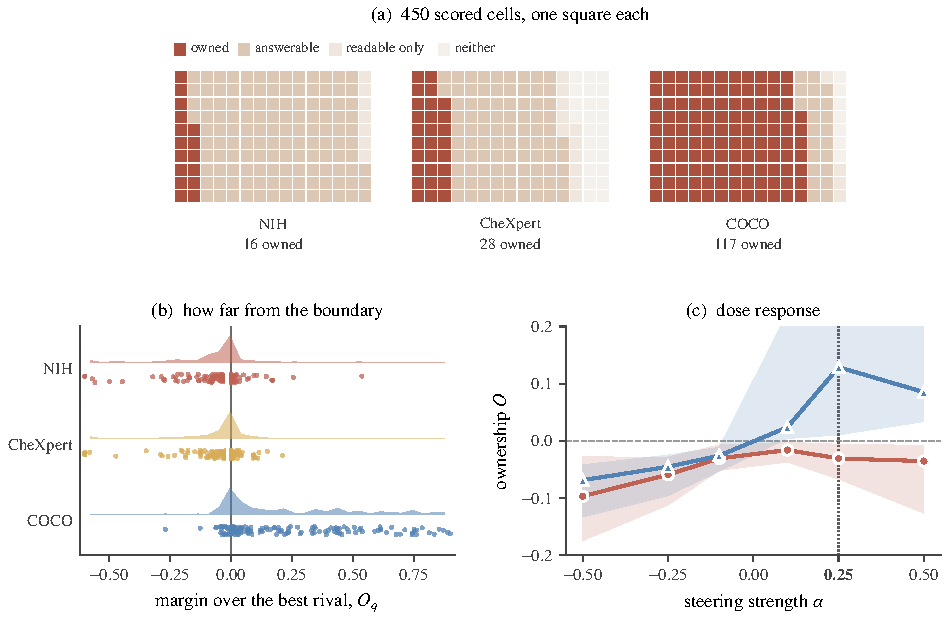
\includegraphics[width=\linewidth]{figures/fig2_overview.pdf}
    \caption{\textbf{Ownership margins by dataset and steering strength.} (a) Distribution of the row margin $O_q$ across checkpoint--concept pairs. (b) Median and interquartile range of $O_q$ by steering strength. The dotted line marks the primary strength.}
    \label{fig:overview}
\end{figure*}

\subsection{Decoding, answering, and control}
\label{sec:headline}

On the two chest datasets, \cfChestReadablePct{}\% of the \cfChestCellsN{} cells were readable and \cfChestAnswerablePct{}\% were answerable. Ownership was less common, at \cfChestOwnedPct{}\% on radiographs and \cfCocoOwnedPct{}\% on COCO (Table~\ref{tab:cf-main}, Fig.~\ref{fig:teaser}). Among the \cfReadAns{} chest cells that passed both reading and answering, only \cfReadAnsOwned{} were owned (\cfReadAnsOwnedPct{}\%). Across steering strengths, the median NIH ownership margin remained negative, while COCO had a positive median at the primary strength (Fig.~\ref{fig:overview}).

\subsection{What the competitor comparison adds}
\label{sec:deficit}

\begin{table}[pos=t]
\centering
\caption{\textbf{Ownership and direction specificity.} Counts of checkpoint--concept pairs. Each of the last three columns requires the steering reference to be met.}
\label{tab:specificity}
\small
\setlength{\tabcolsep}{3pt}
\begin{tabular}{@{}lrrrr@{}}
\toprule
Dataset & \shortstack{Reference\\met} & \shortstack{Owned\\(row)} &
\shortstack{Specific\\(column)} & \shortstack{Owned and\\specific} \\
\midrule
NIH & \jnRefNih & \jnOwnedNih & \jnColSpecNih & \jnTwoWayNih \\
CheXpert Plus & \jnRefChex & \jnOwnedChex & \jnColSpecChex & \jnTwoWayChex \\
Chest total & \jnRefChest & \jnOwnedChest & \jnColSpecChest & \jnTwoWayChest \\
COCO & \jnRefCoco & \jnOwnedCoco & \jnColSpecCoco & \jnTwoWayCoco \\
\bottomrule
\end{tabular}
\end{table}

On chest radiographs, \cfChestRefBelow{} of \cfChestCellsN{} label directions failed the random and sham reference. The median own effect was \cfMedianWqqNih{} on NIH and \cfMedianWqqChex{} on CheXpert Plus, compared with \cfMedianWqqCoco{} on COCO (Table~\ref{tab:cf-controls}). Across checkpoints, the intended question received \cfOwnShareNih{}\% of the total positive change on NIH and \cfOwnShareChex{}\% on CheXpert Plus, compared with \cfOwnShareCoco{}\% on COCO (Appendix~\ref{app:cf-figures}). The write matrices show that some directions raise several chest answers by similar amounts, while COCO effects tend to concentrate on the intended question (Fig.~\ref{fig:write-matrices}).

The reference alone would certify \jnRefChest{} of \cfChestCellsN{} chest directions. Requiring each direction to win on its own question excluded \jnRefLostChest{}. Requiring it also to affect its own answer more than every other answer excluded \jnOwnedNotColChest{} of the \cfChestOwned{} remaining directions. Thus \jnRefNotTwoWayChest{} of the \jnRefChest{} chest directions that passed the reference (\jnRefNotTwoWayChestPct{}\%) failed at least one of the two concept comparisons. On COCO, every direction that met the reference also passed the row comparison, and \jnOwnedNotColCoco{} of \jnRefCoco{} (\jnRefNotTwoWayCocoPct{}\%) failed the column comparison. Overall, \jnTwoWayChest{} of \cfChestCellsN{} chest cells (\jnTwoWayChestPct{}\%) were owned and specific, comprising \jnTwoWayNih{} of \cfNihCells{} on NIH and \jnTwoWayChex{} of \cfChexCells{} on CheXpert Plus. On COCO, \jnTwoWayCoco{} of \cfCocoCells{} (\jnTwoWayCocoPct{}\%) passed both comparisons (Table~\ref{tab:specificity}).

Among directions that met the steering reference, the sum of absolute changes across the other five answers was a median of \jnOffTargetChest{} times the own effect on chest radiographs and \jnOffTargetCoco{} times on COCO. Across all directions, median column selectivity was \jnKappaMedChest{} on chest radiographs and \jnKappaMedCoco{} on COCO (Eq.~\ref{eq:column-selectivity}).

\begin{figure*}[pos=t]
    \centering
    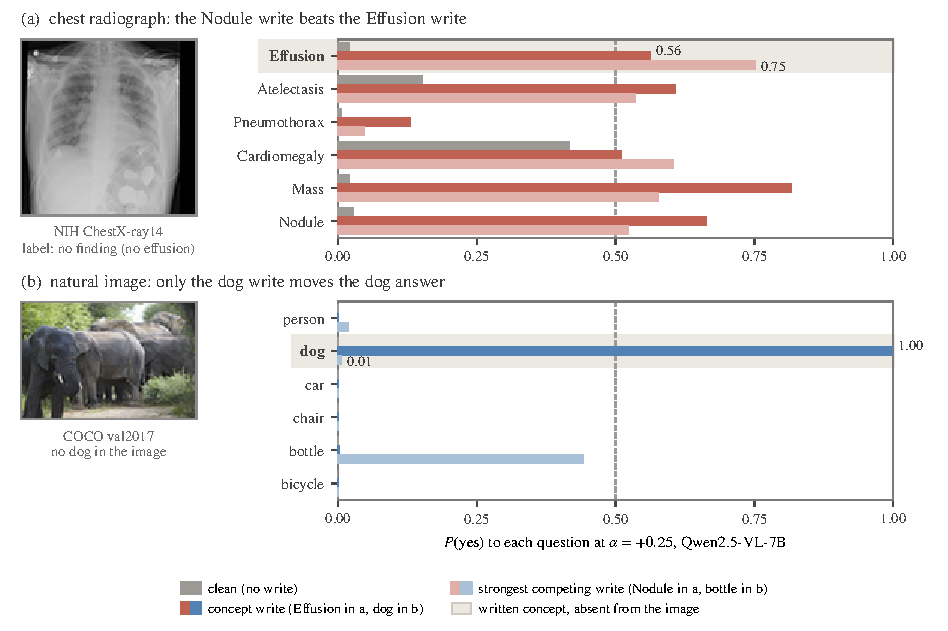
\includegraphics[width=\linewidth]{figures/fig3_example.pdf}
    \caption{\textbf{Answer changes on a radiograph and a photograph.} Qwen2.5-VL-7B's probability of answering yes to each question is shown before editing and after adding the target or strongest competing direction. Shading marks the target question. The dashed line marks equal support for yes and no.}
    \label{fig:example}
\end{figure*}

\label{sec:seed}
The effusion answer again moved more under the nodule write in an independent NIH test cohort ($O_{\mathrm{Effusion}}=\cfSeedEffO$; Table~\ref{tab:cf-seed}). Across chest blocks, \cfEffusionOwnedBlocks{} of \cfChestBlocks{} effusion answers were owned. On the radiograph in Fig.~\ref{fig:example}, the probability of a yes answer for effusion rose from \cfExChestClean{} to \cfExChestOwn{} with the effusion direction and to \cfExChestComp{} with the nodule direction. On the photograph, the dog direction raised the dog answer from \cfExCocoClean{} to \cfExCocoOwn{}, with negligible change in the other answers.

\subsection{Sensitivity to competitors and direction construction}
\label{sec:controls}
\label{sec:robust-geometry}

Averaging across all possible choices of one, two, three, and four competitors gave \jnSubOneChest{}, \jnSubTwoChest{}, \jnSubThreeChest{}, and \jnSubFourChest{} owned chest cells, respectively, compared with \cfChestOwned{} using all five. The COCO count stayed at \cfCocoOwned{} for every subset size. Even one randomly chosen competitor left a wide gap between the domains. The strongest competitor matched the most similar direction at about the chance rate, as it did the most frequently co-occurring label (Table~\ref{tab:cf-geometry}). Adding the other eligible labels to the chest competitor set retained \cfExtcompRetained{} of \cfExtcompOwned{} originally owned cells in the blocks tested.

In owned cells, ranks ranged from \jnOwnedRankMin{} to \jnOwnedRankMax{} when the label write was compared with its \jnRandomDirections{} random reference writes (Fig.~\ref{fig:rank}). Alternative directions fitted from class means, from the feature pattern associated with the probe, or after removing information shared with other concepts yielded ownership rates of \cfAltdirChestPctMin{}--\cfAltdirChestPctMax{}\% on the chest datasets and \cfAltdirCocoPctMin{}--\cfAltdirCocoPctMax{}\% on COCO (Table~\ref{tab:cf-altdir}). The ownership grade agreed with the original evaluation in \cfValidOwnedAgree{} of \cfValidCells{} cells when evaluated on a separate set of \cfValidRows{} CheXpert films with radiologist consensus labels. Refit directions trained on those labels were owned in \cfValidfitOwnedExpert{} of \cfValidfitCells{} cells, compared with \cfValidfitOwnedReport{} for directions trained on report labels. Repeating the probe fit preserved ownership on both refits in \cfRefitGradeStableNih{} of \cfRefitGradeOwnedNih{} owned NIH cells and \cfRefitGradeStableCoco{} of \cfRefitGradeOwnedCoco{} owned COCO cells (Table~\ref{tab:cf-refit}).

\subsection{Ownership at comparable answer difficulty}
\label{sec:coco}

Across checkpoints tested with both sets of COCO categories, the fine-grained objects had a lower median clean-answer AUROC than the common objects (\cfFgFineAuroc{} versus \cfFgEasySameAuroc{}). Fine-grained objects were owned in \cfFgFineOwned{} of \cfFgFineCells{} cells, compared with \cfFgEasySameOwned{} of \cfFgEasySameCells{} for common objects (Appendix~\ref{app:cf-difficulty}). In the highest AUROC stratum (AUROC $\geq\cfStratTopEdge$), \cfStratChestTopOwned{} of \cfStratChestTopN{} chest cells were owned, compared with \cfStratNatTopOwned{} of \cfStratNatTopN{} natural-image cells. The chest-minus-natural difference was \jnTopDiff{} (bootstrap standard deviation \jnTopDiffSd{}). Most chest cells in that stratum came from CheXpert Plus.

The lower common-support cutoff included \jnCsEightyChestN{} chest cells, of which \jnCsEightyChestOwned{} (\jnCsEightyChestPct{}\%) were owned, and \jnCsEightyNatN{} natural-image cells, of which \jnCsEightyNatOwned{} (\jnCsEightyNatPct{}\%) were owned. NIH contributed \jnCsEightyNihN{} of the chest cells and \jnCsEightyNihOwned{} owned cells. After adjustment for clean-answer AUROC and probe selectivity, the chest-minus-natural difference in ownership probability was \jnCsEightyAdj{} (bootstrap standard deviation \jnCsEightyAdjSd{}). At the higher cutoff, the adjusted difference was \jnCsEightyFiveAdj{} (bootstrap standard deviation \jnCsEightyFiveAdjSd{}).

\subsection{Non-clinical attributes of the same radiographs}
\label{sec:attributes}

The probes distinguished projection, recorded sex, and age at least as well as clinical findings on the same radiographs. Median probe AUROC was \cfAttrAurocMin{}--\cfAttrAurocMax{} for the attributes and \cfAttrClinAuroc{} for findings (Appendix~\ref{app:cf-attributes}). With both types of direction included in the comparison, \cfAttrAllAttrOwned{} of \cfAttrAllAttrN{} attribute cells were owned, as were \cfAttrAllClinOwned{} of \cfAttrAllClinN{} finding cells. In the highest clean-answer AUROC stratum of this comparison, \cfStratAttrTopOwned{} of \cfStratAttrTopN{} attribute cells and \cfStratFindTopOwned{} of \cfStratFindTopN{} finding cells were owned.

\subsection{Effects of the components downstream of the vision tower}
\label{sec:reader}

Checkpoints that shared a vision tower and used the same directions differed in which answers those directions controlled (Fig.~\ref{fig:readers}). Ownership margins differed by more than the typical variation across probe refits in \cfPairsRatioAboveOne{} of \cfPairsRatioN{} shared-tower comparisons (Table~\ref{tab:cf-pairs}). The differences persisted when both readers received identical image features.

The crossed Gemma and MedGemma experiment exchanged the reader or the tower while holding the other component fixed. On NIH, the mean absolute change in $O_q$ was \cfSwapReaderNihOMin{} for a reader swap and \cfSwapTowerNihOMin{} for a tower swap. For $W_{q,q}$, the corresponding changes were \cfSwapReaderNihMin{} and \cfSwapTowerNihMin{}. On COCO, the tower swap had the larger effect on $O_q$ (\cfSwapTowerCocoOMin{} versus \cfSwapReaderCocoOMin{}). Across the \cfSwapCombos{} tower--reader combinations, \cfSwapChestOwned{} of \cfSwapChestCells{} chest cells were owned, compared with \cfSwapCocoOwned{} of \cfSwapCocoCells{} COCO cells (Appendix~\ref{app:cf-crossed-reader}).

When the write was applied after the connector, the median ownership margin remained negative on NIH and CheXpert Plus and positive on COCO (Table~\ref{tab:cf-controls}). At that site the edit bypassed the connector, and the language model alone reproduced the sign pattern. Models with chest-trained towers had a higher median NIH probe AUROC than the other checkpoints (\cfSpecTowerProbeAuroc{} versus \cfSpecRestProbeAuroc{}) and owned \cfSpecTowerOwned{} of \cfSpecTowerN{} chest cells. The effect of model size varied across families and findings (Fig.~\ref{fig:ladders}).

\subsection{Control of the model's answer}
\label{sec:ansdir}

The answer direction was owned in \cfAnsChestOwnedA{} of \cfAnsChestN{} chest cells, compared with \cfAnsChestOwnedLabel{} for the label direction (Table~\ref{tab:cf-ansdir}). Higher ownership was expected because we fitted this direction to the model's answers. The two directions were nearly perpendicular on chest radiographs, with a median cosine of \cfAnsCosChestMed{}, and aligned more closely on COCO, with a median cosine of \cfAnsCosCocoMed{}.

On chest radiographs, the answer direction gave a median AUROC of \cfValAurocAnsCleanChest{} against the model's clean answers and \cfValAurocAnsChest{} against the report labels. The label direction gave \cfValAurocProbeCleanChest{} and \cfValAurocProbeChest{}, respectively (Table~\ref{tab:cf-validation}). The answer direction changes the model's output along a signal with weaker agreement with the report labels. Its effect on output is evidence of answer control, and clinical interpretation would require agreement with independently established findings. The ownership advantage also appeared across the tests of negated questions, forced choices, and report continuations (\cfSemAnswerOwned{} of \cfSemCells{} cells for answer directions versus \cfSemLabelOwned{} for label directions; Table~\ref{tab:cf-semend}).

\FloatBarrier

\section{Discussion}
\label{sec:implications}

Label directions were both owned and specific in \jnTwoWayChestPct{}\% of checkpoint--concept pairs on chest radiographs and \jnTwoWayCocoPct{}\% on COCO. Half of the chest directions that cleared the random and sham references failed at least one of the labeled comparisons. Ownership was less common on chest radiographs at comparable answer difficulty. Projection, recorded sex, and age showed similarly low ownership despite being easier to decode than findings on the same images.

Ravichander et al.\cite{ravichander2021probing} showed that information recovered by a probe can go unused by the model. Arad et al.\cite{arad2025saes} showed that different internal features can detect a concept and control its output. Haufe et al.\cite{haufe2014interpretation} distinguished classifier weights from the activation patterns associated with the signal they detect. Marks and Tegmark\cite{marks2024geometry} found that a direction based on the difference between class means steered truth judgments more reliably than a probe direction. RAW extends this work by testing specificity against labeled competitors. Across \cfCheckpoints{} checkpoints, most chest directions failed the joint ownership and specificity test, while most COCO directions passed.

Checkpoints given identical visual features and directions differed in ownership, showing that the components downstream of the vision tower affect which findings a direction controls. The language model reproduced the chest and COCO sign pattern when it received the edit after the connector. The answer-fitted directions on radiographs agreed more closely with model answers than with report labels. Clinical interpretation requires checking how an output change relates to the annotated finding.

For radiology AI audits, report the full write matrix. Compare each clinical direction with labeled competitors on the intended answer and measure its effects on the other answers. Apply the same evaluation to a natural-image control to check that it detects selective control where it occurs.

\label{sec:limitations}
This study used frontal chest radiographs with report-derived labels from NIH ChestX-ray14 and CheXpert Plus, supplemented by a CheXpert consensus-label analysis, and COCO photographs as a control. RAW applies to open-weight VLMs whose activations can be accessed. The grades characterize short answers under the edits and labeled concepts evaluated here.

\section{Conclusions}
\label{sec:conclusion}

Chest findings were often readable and answerable in the models studied. Few chest directions selectively controlled their intended answers. Labeled comparisons halved the number of chest directions that passed random and sham controls. RAW identifies which directions selectively control the intended answer within the findings tested.

\section*{CRediT authorship contribution statement}
The authors' contributions are as follows. \textcolor{red}{[Confirm the CRediT roles for each author.]}

\section*{Ethics statement}
This study is a secondary analysis of publicly available, de-identified datasets. NIH ChestX-ray14 was released by the NIH Clinical Center for public research use, and CheXpert Plus was obtained from the Stanford Center for Artificial Intelligence in Medicine and Imaging under its research data use agreement; both datasets were de-identified by their providers before release. COCO images and annotations were used under the dataset's terms of use. The authors had no access to protected health information, did not attempt to re-identify any individual, and redistribute no radiographs or reports. Because the study involved no interaction with human participants and used only de-identified public data, institutional review board approval and informed consent were not required.

\section*{Declaration of competing interest}
The authors declare that they have no known competing financial interests or personal relationships that could have appeared to influence the work reported in this paper.

\section*{Funding}
This work was supported by \textcolor{red}{[confirm funders, grant numbers, and funder roles, or state that this research received no specific grant]}.

\section*{Data and code availability}
NIH ChestX-ray14, CheXpert Plus, and COCO are available from their providers subject to the applicable access terms.\cite{wang2017chestxray,chambon2024chexpertplus,lin2014coco} The RAW code is publicly available in the \href{https://github.com/hq0709/reading-is-not-writing-code}{RAW GitHub repository}. Section~\ref{app:repro} documents registration and the materials available for reproduction.

\section*{Declaration of generative AI and AI-assisted technologies in the writing process}
During the preparation of this work, the authors used Codex (OpenAI) and Claude (Anthropic) to check grammar and polish the language. After using these tools, the authors reviewed and edited the content as needed and take full responsibility for the content of the published article.


\begingroup
\raggedright
\bibliographystyle{vancouver-mr}
\bibliography{refs}
\endgroup

\end{document}
